%Kompiliuoti su XeLaTeX ir BibTeX

\documentclass[a4paper, 12pt, oneside]{article}

\usepackage[yyyymmdd]{datetime}

\usepackage{fontspec}
\usepackage{fontenc}
\usepackage{ulem}
\usepackage{cite}
\usepackage{mathtools}
\usepackage{amsmath}
\usepackage{amssymb}
%\usepackage{float}
\usepackage{graphicx}
\usepackage{multirow}
\usepackage[hyphens]{url}
\usepackage{caption}
\usepackage{subcaption}
\usepackage[svgnames]{xcolor}
\usepackage{lineno}
\usepackage[lithuanian]{babel}
\usepackage{hyperref}
\usepackage{siunitx}
\usepackage{floatrow}
\usepackage{indentfirst}
%\usepackage[parfill]{parskip}

\floatsetup[table]{capposition=top}

\hypersetup{breaklinks=true}
\urlstyle{same}

\usepackage{geometry}
\pagestyle{myheadings}
\geometry{
	left=3cm,
	right=1cm,
	top=2cm,
	bottom=2cm,
}
\pagenumbering{arabic}
\linespread{1.25}

\graphicspath{ {images/} }

\renewcommand{\dateseparator}{-}
\addto\captionslithuanian{\renewcommand{\figurename}{pav}}
\addto\captionslithuanian{\renewcommand{\refname}{6 \hspace{0.1cm} Naudotos literatūros sąrašas}}
\addto\captionslithuanian{\renewcommand{\tablename}{lentelė}}

\DeclareCaptionLabelFormat{numfirst}{#2~#1}
\captionsetup[figure]{labelformat = numfirst, labelsep = period}
\captionsetup[table]{labelformat = numfirst, labelsep = period}

\newcommand{\textblue}[1]{{\color{Blue}#1}}
\newcommand{\textred}[1]{{\color{Red}#1}}
\newcommand{\comment}[1]{\newline\textblue{#1}\newline}
\newcommand{\commentNL}[1]{\textblue{#1}\newline}
\newcommand{\commentMA}[1]{\textred{#1}\newline}
\newcommand{\ttt}[1]{\texttt{#1}}
\newcommand{\pT}{p_{\mathrm{T}}}
\newcommand{\ET}{E_{\mathrm{T}}}
\newcommand{\WW}{W\! W}
\newcommand{\ZZ}{Z\! Z}
\newcommand{\WZ}{W\! Z}
\newcommand{\tbarW}{\bar{t}W}
\newcommand{\ttbar}{t\bar{t}}
\newcommand{\emu}{e\mu}
\newcommand{\mumu}{\mu\mu}
\newcommand{\gJets}{\gamma\! +\!\mathrm{Jets}}
\newcommand{\WJets}{W\! +\!\mathrm{Jets}}
\newcommand{\dtW}{tW\! + \! \bar{t}W}
\newcommand{\DYee}{\mathrm{DY} \! \rightarrow \! ee}
\newcommand{\DYmumu}{\mathrm{DY} \! \rightarrow \! \mu\mu}
\newcommand{\DYtau}{\mathrm{DY} \! \rightarrow \! \tau\tau}
\newcommand{\DY}{\mathrm{DY}}
\newcommand{\ltq}[1]{{\quotedblbase{}#1\textquotedblleft{}}}
\newcommand{\Lumi}{{\cal L}_\mathrm{int}}
\newcommand{\invfb}{fb$^{-1}\,$}
\newcommand{\invpb}{pb$^{-1}\,$}
\newcommand{\QCD}{QC\! D}

\newlength\q
\setlength\q{\dimexpr .5\textwidth -2\tabcolsep}

\hyphenation{eks-pe-ri-men-tą}
\hyphenation{so-le-noi-das}
\hyphenation{Feinmano}
\hyphenation{ha-dro-no}
\hyphenation{MadGraph}
\hyphenation{už-re-gis-truo-tų}
\hyphenation{miu-o-nų}
\hyphenation{in-te-gruo-tą-jį}
\hyphenation{eks-pe-ri-men-ti-nių}
\hyphenation{alice}
\hyphenation{so-le-noi-di-nis}
\hyphenation{pythia}

\begin{document}
%\linenumbers

\begin{titlepage}
\centering
{\large Vilniaus universiteto \\ Fizikos fakulteto \\ Teorinės fizikos ir astronomijos institutas \par}
\vspace{3.5cm}
{\Large Marijus Ambrozas \par}
\vspace{0.3cm}
{\Large Drell-Yan proceso triukšmo įvykių skaičiaus įvertinimas klaidingo atpažinimo metodu\par}
\vspace{0.8cm}
{\large Magistrantūros studijų baigiamasis darbas \par}
\vspace{0.8cm}
{\large Teorinės fizikos ir astrofizikos \\ studijų programa \par}
\vspace{3.5cm}
{\large \begin{tabular*}{0.9\textwidth}{@{\extracolsep{\fill}}ll}
Studentas & Marijus Ambrozas\tabularnewline[0.5cm]
Darbo vadovas & dr.\ Andrius Juodagalvis\tabularnewline[0.5cm]
Instituto atstovas & prof.\ Egidijus Anisimovas\tabularnewline[0.5cm]
\end{tabular*} \par}
\vspace{4cm}
{\large Vilnius $2020$\par}
\end{titlepage}


\clearpage
\addtocounter{page}{1}
\addtocontents{toc}{\protect\setcounter{tocdepth}{2}}
\tableofcontents
\clearpage

\section*{Įvadas} \addcontentsline{toc}{section}{Įvadas}
Hadronų sandaros aprašymui didelių energijų fizikoje šiais laikais plačiai naudojamas R.\ Feinmano pasiūlytas
partonų modelis \cite{FeynPartons}.
Šiame modelyje visų hadronų sandara nusakoma partonų pasiskirstymo funkcijomis \cite{BjorkPartons}.
Tikslus partonų pasiskirstymo funkcijų žinojimas yra svarbus stengiantis suprasti didelės energijos protonų susidūrimų
metu vykstančius procesus.
Šias funkcijas teoretikų grupės nuolat tikslina, priderindamos jas prie naujausių eksperimentinių tyrimų rezultatų
\cite{PDF_MMHT2015, PDF_CJ15, NNPDF, PDF_ABMP16, PDF_MMHT2019, CTEQ2019}.

Vienas iš \ltq{švariausių} procesų, suteikiančių svarbios informacijos apie protono sudėtį, yra
Drell-Yan procesas \cite{DYoriginal}.
Tai -- didelės energijos protonų susidūrimo metu vykstantis procesas, kai kvarkas iš vieno protono ir antikvarkas
iš kito anihiliuoja sukurdami leptono ir antileptono porą.
Naujausi Drell-Yan proceso diferencialinio reakcijos skerspjūvio matavimai pasižymi dideliu tikslumu
\cite{DY_CMS2013, DY_ATLAS2013, DY_ATLAS2014, DY_CMS2015, DY_ATLAS2016, DY_ATLAS2017, DY_CMS2019}.
Šių matavimų rezultatai naudojami tikslinant partonų pasiskirstymo funkcijas bei testuojant perturbatyvų standartinio
modelio aprašymą.
Drell-Yan proceso tyrimas svarbus ir kitus didelių energijų fizikos procesus tiriantiems eksperimentatoriams,
kurių matavimams šis procesas trukdo \cite{Higgs2018, Zprime, SUSYtau}.
Taigi, Drell-Yan proceso tyrimai užima svarbią vietą eksperimentinėje didelių energijų fizikoje.

CERN Didysis hadronų greitintuvas protonus sudaužia $40$ milijonų kartų per sekundę, susidūrimų energijai masių
centro sistemoje siekiant $13$ TeV.
Protonų susidūrimo metu gali būti sukuriamos labai trumpai gyvuojančios masyvios dalelės, tokios, kaip
$Z$, $W$, Higso bozonai ir kt.
Aplink protonų susidūrimo taškus pastatyti dalelių detektoriai registruoja tik tokių dalelių skilimo produktus:
elektronus, miuonus, fotonus bei įvairių rūšių hadronus.
Užregistruoti protonų susidūrimai, kurių metu buvo sukurti du izoliuoti (aplink save neturintys pašalinių dalelių
trajektorijų) priešingo krūvio leptonai, vadinami Drell-Yan proceso įvykio kandidatais.
Vienareikšmiškai pasakyti, kokio proceso metu susidarė detektoriaus užregistruotos dalelės, yra neįmanoma:
visada egzistuoja keli skirtingi procesai, kuriems užregistruotas įvykio vaizdas gali atrodyti labai panašiai.
Taip tarp Drell-Yan proceso įvykių kandidatų patenka ir su pašaliniais procesais susiję įvykiai.
Jie vadinami triukšmo įvykiais.
Iš įvykių rinkinio triukšmai pašalinami statistiškai: bandoma įvertinti, kokia jo dalis yra užteršta.
Grubų triukšmo įvykių skaičiaus įvertį galima gauti naudojantis sumodeliuotais protonų susidūrimais.
Vis dėlto, siekiant tikslesnės detektoriaus išmatuotų pasiskirstymų interpretacijos, naudojami matavimu grįsti
triukšmo įvykių skaičiaus įvertinimo metodai.
Šiame darbe buvo naudojamas klaidingo atpažinimo metodas, kuris taikomas įvertinant indėlį tokių triukšmų, kuriuose
įvykiai su klaidingai atpažintomis hadronų čiurkšlėmis pateko tarp Drell-Yan proceso įvykių kandidatų.

\textbf{Šio darbo tikslas} -- įvertinti Drell-Yan proceso triukšmo įvykių skaičių klaidingo atpažinimo metodu.
Tikslui pasiekti iškelti tokie uždaviniai:
1) Įvertinti tikimybę, kad čiurkšlės gali būti klaidingai atpažintos kaip izoliuoti miuonai ir elektronai;
2) Pritaikyti klaidingo atpažinimo tikimybių įverčius nustatant, kiek Drell-Yan proceso įvykių kandidatų yra susiję su
klaidingai atpažintomis čiurkšlėmis;
3) Įvertinti gauto rezultato statistinius ir sisteminius neapibrėžtumus.
Darbe buvo naudojami CERN CMS eksperimento 2016 metais užregistruoti protonų susidūrimų duomenys.


\section{Drell-Yan proceso tyrimas CMS eksperimente}
Šiame skyriuje supažindinama su didelių energijų fizikoje naudojamu protono sandaros aprašymu ir Drell-Yan procesu.
Trumpai pristatomos pagrindinės šio proceso tyrimo kryptys ir paaiškinama jų svarba.
Toliau supažindinama su didelių energijų fizikos tyrimuose naudojama eksperimentine įranga, trumpai paaiškinama,
kaip gaunami fizikinei analizei naudojami duomenys.
Taip pat šiame skyriuje aptariama su darbo tikslu susijusi eksperimentinių didelių energijų fizikos tyrimų problematika,
supažindinama su tyrime naudojamomis signalo ir triukšmo sąvokomis bei pristatomas klaidingo atpažinimo metodas,
kuris buvo taikomas atliekant darbą.

\subsection{Partonų pasiskirstymo funkcijos}
Standartiniame modelyje procesus nusakantys pamatuojami dydžiai (reakcijos skerspjūvis, skilimo dažnis) aprašomi sąveikos
konstantos laipsnių eilute, kurios kiekvieną narį galima pavaizduoti atitinkamomis Feinmano diagramomis.
Kad toks perturbatyvus aprašymas veiktų, sąveikos konstanta turi būti gerokai mažesnė už vienetą.
Iš renormalizacijos seka, kad sąveikos konstantos turi logaritminę priklausomybę nuo reakcijos metu pernešamos energijos.
Dėl šios priežasties skirtingos sąveikos perturbatyviai gali būti aprašomos tik tam tikrose energijų srityse\cite{QCDalpha}.

Kvantinė chromodinamika (angl. \textit{quantum chromodynamics} -- QCD) aprašo stipriąją sąveiką, kuri vienija hadronus
sudarančias daleles: kvarkus ir gliuonus.
Jei kvarkams ir gliuonams sąveikaujant energijos pernaša yra labai maža (pavyzdžiui, vyksmams atomo branduolyje),
stipriosios sąveikos konstanta $\alpha_s$ yra labai didelė.
Dėl šios priežasties perturbatyvus aprašymas žemų energijų stipriesiems procesams yra netinkamas.
Vis dėlto, stiprioji sąveika pasižymi asimptotine laisve (angl.\ \textit{asymptotic freedom}) -- reakcijos metu pernešamai
energijai didėjant sąveikos konstanta mažėja, o pasiekus begalinę energiją dalelės turėtų nebesąveikauti išvis \cite{AFreedom}.
Pavyzdžiui, jei sąveika tarp susiduriančių protonų sudedamųjų dalių -- kvarkų -- yra ekvivalenti $Z$ bozono masei ($91.2$~GeV),
stipriosios sąveikos konstanta jau turi vertę, siekiančią vos $0.118$ \cite{PDGreview}.
Asimptotinė laisvė leidžia šiuolaikiniuose dalelių greitintuvuose vykstančių procesų teoriniams įverčiams naudoti
perturbatyvų aprašymą.

Norint teoriškai aprašyti hadronų susidūrimus svarbu žinoti, kokios yra tikimybės, kad sąveikaus konkrečios
hadrono viduje esančios dalelės.
Šiam tikslui yra naudojamas R.~Feinmano pasiūlytas artinys, vadinamas partonų modeliu \cite{FeynPartons}:
kai energijos pernaša reakcijos metu yra tokia didelė, kad būtų galima taikyti perturbatyvų kvantinės chromodinamikos aprašymą,
hadrono sudedamųjų dalių -- partonų -- impulso dedamosios, statmenos hadrono judėjimo krypčiai, yra nykstamai mažos,
lyginant su lygiagrečia hadrono judėjimui dedamąja.
Tai reikštų, kad su hadronu susiduriančios dalelės atskaitos sistemoje hadroną galime įsivaizduoti kaip plokščią nejudančių
taškų rinkinį.
Toks artinys pilnai atitiktų realybę, jeigu hadrono impulsas būtų begalinis.
Pritaikius partonų modelį hadroną galima aprašyti kaip tikimybės tankių rinkinį: kiekviena rinkinyje esanti funkcija nusakytų tikėtinumą
aptikti konkretų partoną (kvarką arba gliuoną), nešantį tam tikrą procentinę hadrono impulso dalį $x$ \cite{BjorkPartons}.
Šie tikimybės tankiai vadinami partonų pasiskirstymo funkcijomis (angl.\ \textit{parton distribution function} -- PDF).
Partonų pasiskirstymo funkcija $f_{i}(x, Q^{2})$ aprašo tikimybę aptikti $i$ tipo partoną (pavyzdžiui, kylantįjį kvarką -- $u$,
krentantįjį kvarką -- $d$ ir t.t.), nešantį tam tikrą protono impulso dalį tarp $x$ ir $x\!+\!\mathrm{d}x$, kai \textit{kietojo}
susidūrimo energija lygi $Q$.
Kietasis susidūrimas (angl.\ \textit{hard interaction}) -- procesas, kurio metu vyksta energijos pernaša, palyginama
su pilnąja sistemos energija.
Du partonų pasiskirstymo funkcijų pavyzdžiai, esant skirtingoms pernašos energijoms, yra pateikti
\ref{fig:PDFs} paveiksle.

Hadronų susidūrimų metu vykstančių reakcijų skerspjūviai $\sigma$ yra apskaičiuojami kaip partonų pasiskirstymo
funkcijų $f_i$ ir partonų tarpusavio reakcijos skerspjūvio $\hat{\sigma}$ kombinacija:
\begin{equation}
	\sigma = \sum_{i, j} \int \mathrm{d}x_1 \int \mathrm{d}x_2 \,
	f_{i}(x_1, \, Q^2) \, f_{j}(x_2 \, Q^2) \, \hat{\sigma}(x_1 p_1, \, x_2 p_2, \, Q^2) \; \mathrm{,}
	\label{eq:PDFxsec}
\end{equation}
čia $\sigma$ -- reakcijos skerspjūvis, $i$, $j$ -- sąveikaujantys partonai, nešantys protonų impulsų $p_1$ ir $p_2$
dalis $x_1$ ir $x_2$, o $f_{i}(x_1, \, Q^2)$ ir $f_{j}(x_2, \, Q^2)$ -- partonų pasiskirstymo funkcijos, o
$\hat{\sigma}(x_1 p_1, \, x_2 p_2, \, Q^2)$ -- konkrečių partonų su impulsais $x_1 p_1$ ir $x_2 p_2$ tarpusavio
reakcijos skerspjūvis, kai energijos pernaša reakcijos metu lygi $Q$.

\begin{figure}[t]
	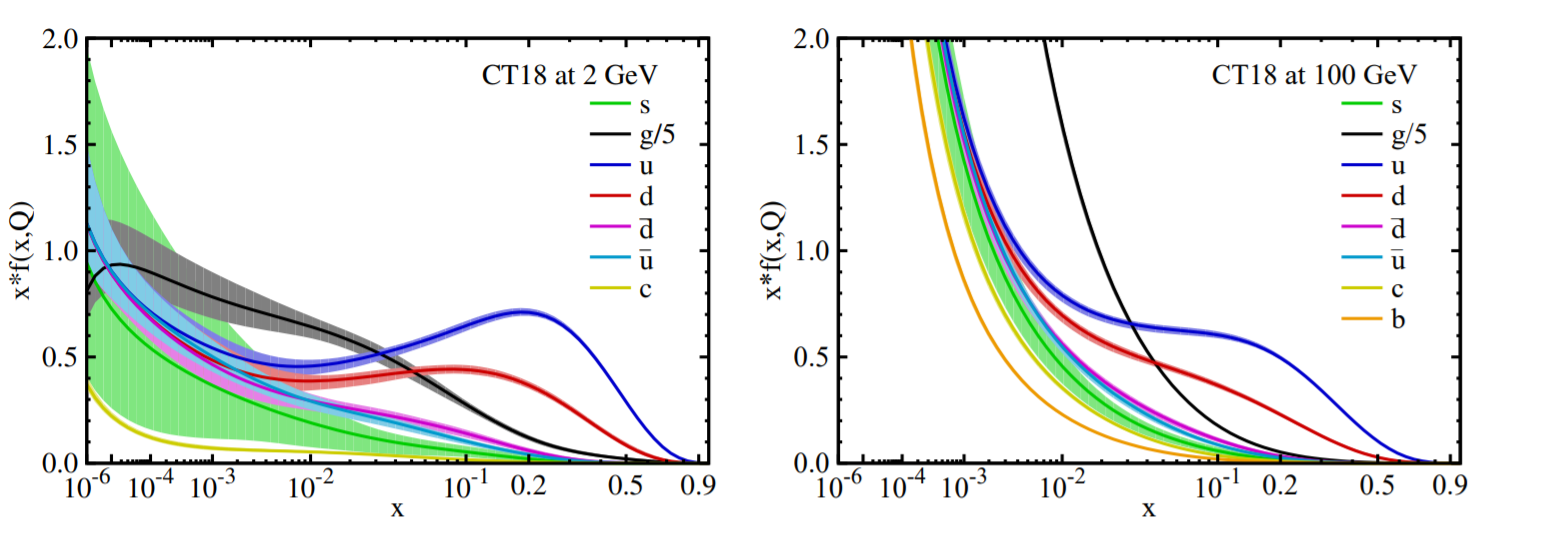
\includegraphics[width=\linewidth]{CT18_PDF.png}
	\caption{\label{fig:PDFs}
		CTEQ-TEA kolektyvo pateikiamos protono partonų pasiskirstymo funkcijos, esant skirtingo dydžio energijoms pernašoms $Q$ \cite{CTEQ2019}.
		Kairėje pusėje $Q=2 \; \mathrm{GeV}$, o dešinėje pusėje -- $Q=100 \; \mathrm{GeV}$.
		Ant horizontalios ašies vaizduojama protono impulso dalis $x$, o ant vertikalios -- tikimybės tankio $f(x,\, Q^2)$
		ir $x$ sandauga.}
\end{figure}

Naudojantis šiuolaikine teorija, partonų pasiskirstymo funkcijų neįmanoma apskaičiuoti iš pirminių principų.
Jos gaunamos skirtingais metodais priderinant funkcijų parametrus prie eksperimentinių tyrimų rezultatų
\cite{PDF_MMHT2015, PDF_CJ15, NNPDF, PDF_ABMP16, PDF_MMHT2019, CTEQ2019}.
Vieni svarbiausių rezultatų, naudojamų partonų pasiskirstymo funkcijų parametrų nustatymui atkeliauja iš elektrono-protono
sklaidos eksperimentų (anksčiau tokius susidūrimus vykdydavo Hamburge esantis dalelių greitintuvas HERA) bei eksperimentiškai nagrinėjant
Drell-Yan proceso, viršūninių kvarkų poros sukūrimo bei vienos čiurkšlės įvykius, kurie vyksta protono-protono priešpriešinių susidūrimų
metu \cite{CTEQ2019}.
%Turint noro išplėsti dalį apie tyrimus


\subsection{Drell-Yan procesas}
Protonams susiduriant su didžiule energija kvarkas iš vieno protono ir antikvarkas iš kito gali anihiliuoti ir sukurti leptono-antileptono
porą -- elektroną, miuoną arba taoną su atitinkama savo antidalele.
Toks procesas vadinamas Drell-Yan procesu, jis vyksta apsikeičiant $Z$ bozonu arba virtualiu fotonu per s-kanalą:

\begin{equation*}
	q\bar{q} \rightarrow Z/ \gamma^{*} \rightarrow l^{+}l^{-} \; ,
\end{equation*}
čia $q$ ir $\bar{q}$ žymi atitinkamai kvarką ir antikvarką, $\gamma^*$ žymi virtualų fotoną, o $l^+$ ir $l^-$ -- atitinkamai
antileptoną ir leptoną.
Šią reakciją toliau žymėsime $\DY \! \rightarrow \! l^{+}l^{-}$.
Skirtingos Drell-Yan proceso galutinės būsenos, priklausomai nuo to, kokios rūšies leptonai susidaro, yra
vadinamos kanalais: elektronų kanalas, miuonų kanalas, taonų kanalas.
Kadangi taonai gyvuoja labai trumpai, jų kanalo tyrimas yra sudėtingesnis ir dažniausiai yra vykdomas atskirai,
o tuo tarpu elektronų ir miuonų kanalo tyrimus neretai vykdo ta pati mokslinė grupė.

Drell-Yan procesas teoriškai pirmą kartą buvo aprašytas $1970$-aisiais metais.
Tai padarė mokslininkai S.~D.~Drell ir T.~M.~Yan, kurie pritaikė neseniai pasiūlytą partonų modelį aprašyti
leptonų poros susidarymui hadronų susidūrimo metu \cite{DYoriginal}.
Drell-Yan procesas pirmą kartą eksperimentiškai buvo stebėtas dar tais pačiais metais protonų susidūrimuose
su urano branduoliais \cite{DY_firstExp}.
Šio proceso tyrimas svarbus todėl, kad jame dalyvauja nevalentinis protono antikvarkas.

Šiais laikais teoretikai Drell-Yan procesą gali sėkmingai aprašyti iki antros eilės (angl.\ \textit{next-to-leading order} -- NLO --
reiškia vienos kilpos ir vienos dalelės išspinduliavimo pataisas) elektrosilpnosios sąveikos
ir trečios eilės kvantinės chromodinamikos perturbacijų tikslumo (angl.\ \textit{next-to-next-to-leading order} -- NNLO --
reiškia dviejų kilpų ir dviejų dalelių išspinduliavimo pataisas).
Apsiribojama antros eilės elektrosilpnosiomis pataisomis, nes kiekvienos elektrosilpnosios viršūnės indėlis į reakcijos skerspjūvį
yra $\sim\!10$ kartų mažiau reikšmingas (dėl atitinkamai mažesnės sąveikos konstantos), lyginant su stipriosios sąveikos viršūne.
Drell-Yan proceso pirmos eilės (angl.\ \textit{leading order} -- LO -- reiškia medžio lygmenį) Feinmano diagramos
yra pavaizduotos \ref{fig:DYfeyn}~pav.
Kai kurios aukštesnių eilių Feinmano diagramos pateikiamos 1 priede.

\begin{figure}[b]
\centering
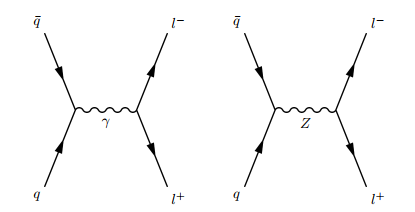
\includegraphics[scale=0.75]{DYprocess.PNG}
\caption{Drell-Yan procesą apibūdinančios medžio lygmens Feinmano diagramos.}
\label{fig:DYfeyn}
\end{figure}

Drell-Yan proceso diferencialinis reakcijos skerspjūvis yra šešiamatis:
$\mathrm{d}^6\sigma/(\mathrm{d}^4p\,\mathrm{d}\theta_{\mathrm{CS}}\mathrm{d}\phi_\mathrm{CS}$), čia $\sigma$ -- reakcijos skerspjūvis,
$p$ -- leptonų poros keturmatis impulsas (lygus tarpinės dalelės -- $Z$ bozono arba virtualaus fotono keturmačiam
impulsui), $\theta_{\mathrm{CS}}$ -- kampas tarp išlekiančio antileptono ir $z$ ašies, o $\phi_{\mathrm{CS}}$ -- azimutinis kampas
Collins-Soper atskaitos sistemoje (virtualaus bozono rimties sistemoje) \cite{DYangular}.
Collins-Soper atskaitos sistema ir kampai $\theta_{\mathrm{CS}}$ bei $\phi_{\mathrm{CS}}$ pavaizduoti \ref{fig:CSframe} pav.
Didelių energijų fizikoje keturmatis impulsas dažnai išreiškiamas kaip masės $m=\sqrt{E^2-|\vec{p}|^2}$ (čia $E$ -- energija,
$\vec{p}$ -- trimatis impulso vektorius), skersinio impulso $\pT=\sqrt{p_x^2+p_y^2}$ (čia $p_x$, $p_y$ -- impulso dedamosios
išilgai ašių, statmenų protonų susidūrimo krypčiai), spartos $y=\frac{1}{2}\mathrm{ln}[\frac{E+p_z}{E-p_z}]$ (čia $p_z$ -- impulso dedamoji
išilgai protonų susidūrimo ašies) ir sferinės koordinačių sistemos azimutinio kampo $\phi$ rinkinys.
Taigi keturmačio impulso diferencialas $\mathrm{d}^4p$ gali būti pakeistas į $\mathrm{d}m\mathrm{d}\pT\mathrm{d}y\mathrm{d}\phi$.
Be to, šie dydžiai apie procesą gali suteikti gerokai naudingesnės informacijos.

\begin{figure}[b!]
	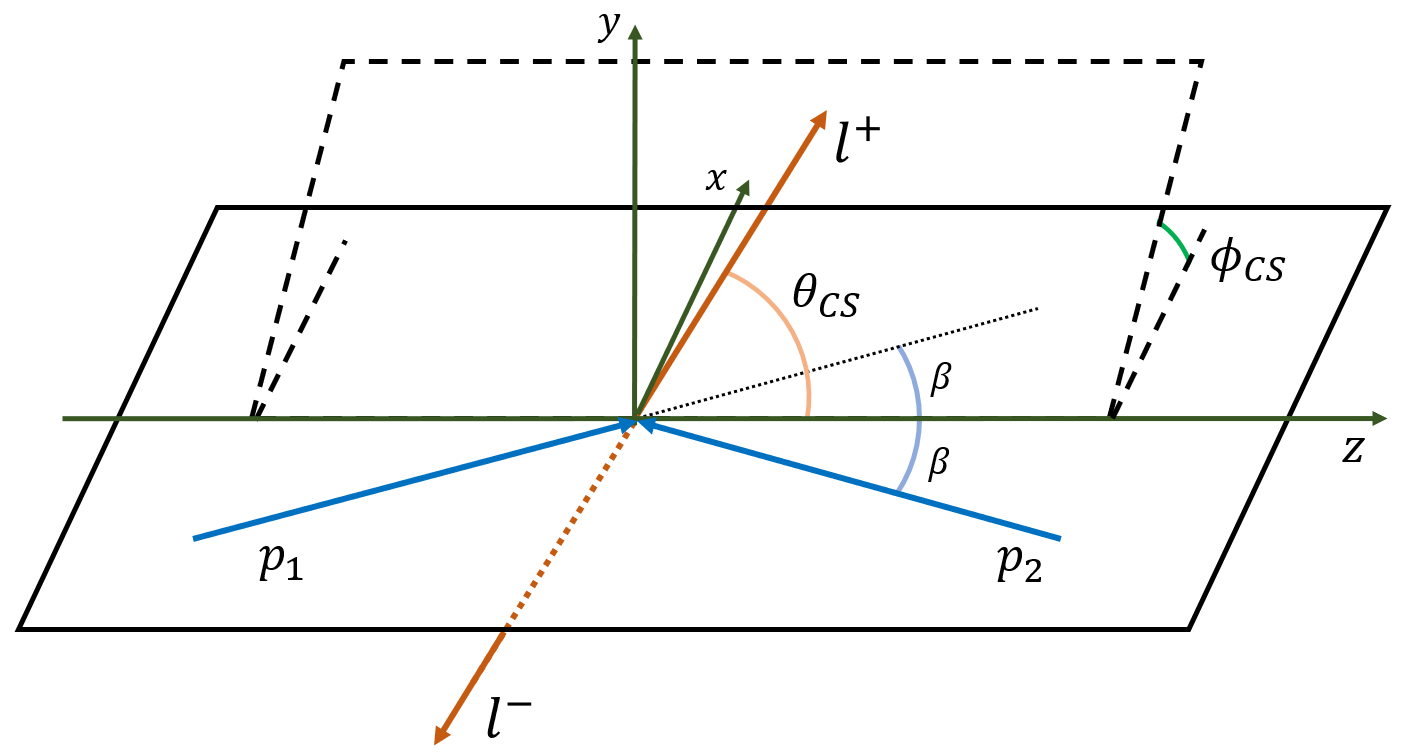
\includegraphics[width=0.7\textwidth]{Magistrinis/CSframe.png}
	\caption{\label{fig:CSframe} Collins-Soper atskaitos sistemos iliustracija.
	Čia $p_1$ ir $p_2$ vaizduoja susiduriančių protonų impulso vektorius, o $l^-$ ir $l^+$ -- išlekiančių leptonų impulso vektorius.
	$z$ ašis brėžiama taip, kad perpus dalintų kampą tarp $p_2$ ir $-p_1$, o $x$ ašis -- lygiagreti $p_1$ ir $p_2$ vektorinei sumai.}
	%$\theta_{\mathrm{CS}}$ atitinka kampą tarp išlekiančio teigiamo krūvio leptono ir $z$ ašies, o $\phi_{\mathrm{CS}}$ -- kampą
	%tarp plokštumos, kurią sudaro protonų impulso vektoriai kartu su $z$ ir $x$ ašimis bei plokštumos, kurią sudaro išlekiančių
	%leptonų impulso vektoriai kartu su $z$ ašimi.}
\end{figure}

Norint pakankamai tiksliai išmatuoti diferencialinio reakcijos skerspjūvio priklausomybę nuo visų šešių parametrų,
reikėtų labai didelio kiekio duomenų, o taip pat ne visos funkcinės priklausomybės yra vienodai svarbios (pavyzdžiui,
priklausomybė nuo azimutinio kampo $\phi$ yra konstanta, todėl tirti šią priklausomybę nėra prasmės).
Todėl dažniausiai matuojami vienmačiai, dvimačiai arba trimačiai Drell-Yan proceso reakcijos skerspjūviai
\cite{DY_comp1993, DY_CDF1994, DY_D01999, DY_CDF2001, DY_comp2007, DY_CMS2011, DY_CMS2013, DY_ATLAS2013, DY_ATLAS2014,
DY_CMS2015, DY_ATLAS2016, DY_ATLAS2017, DY_CMS2019}.
Nuo skirtingų parametrų priklausančių diferencialinių reakcijos skerspjūvių matavimo rezultatai teoretikams teikia
skirtingą informaciją.

Iš kiekvienoje Feinmano diagramos viršūnėje galiojančios energijos ir impulso tvermės seka, kad, idealiai priešpriešinio
protonų susidūrimo metu, Drell-Yan leptonų poros invariantinė masė medžio lygmenyje priklauso vien
tik nuo susiduriančių protonų impulsų dalių, kurias neša sąveikaujantys partonai.
Laužtiniuose skliaustuose pateikdami keturmačio impulso komponentes $(E,p_x,p_y,p_z)$, galime užrašyti:
\begin{align}
\label{eq:DY4vec}
	\begin{bmatrix}
		x_1p_{z\,1} \\		
		0 \\
		0 \\
		x_1p_{z\,1} \\
	\end{bmatrix}
	+
	\begin{bmatrix}
		x_2p_{z\,2} \\
		0 \\
		0 \\
		-x_2p_{z\,2} \\
	\end{bmatrix}
	=
	\begin{bmatrix}
		E_{(\gamma^*\!/\!Z)} \\
		0 \\
		0 \\
		p_{z\,(\gamma^*\!/\!Z)} \\
	\end{bmatrix}
	=
	\begin{bmatrix}
		E_{l1} \\
		p_{x} \\
		p_{y} \\
		p_{z\,l1} \\
	\end{bmatrix}
	+
	\begin{bmatrix}
		E_{l2} \\
		-p_{x} \\
		-p_{y} \\
		p_{z\,l2} \\
	\end{bmatrix}	
	,
\end{align}
iš čia seka, kad
\begin{equation}
\label{eq:DYinvm}
	m^2_{ll} = (E_{l1}+E_{l2})^2-(p_{z\,l1}+p_{z\,l1})^2 = m^2_{(\gamma^*\!/\!Z)} = E^2_{(\gamma^*\!/\!Z)}-p^2_{z\,(\gamma^*\!/\!Z)} =
	(x_1p_{z\,1}+x_2p_{z\,2})^2-(x_1p_{z\,1}-x_2p_{z\,2})^2 ,
\end{equation}
čia $p_{z\,1}$ ir $p_{z\,2}$ -- susiduriančių protonų impulsai (absoliutinės vertės), $x_1$ ir $x_2$ -- sąveikaujančių partonų nešamos
tų protonų impulsų dalys, (čia laikome, kad kvarko masė lygi nuliui, todėl jo energija apytiksliai lygi impulso moduliui, o minusu
pažymime, kad protonai atlekia iš priešingų pusių), $E_{(\gamma^*\!/\!Z)}$ -- $Z$ bozono arba virtualaus fotono energija,
$p_{z\,(\gamma^*\!/\!Z)}$ -- $Z$ bozono arba virtualaus fotono impulsas, $E_{l1}$, $p_{z\,l1}$, $E_{l2}$ ir $p_{z\,l2}$ -- susidariusių
leptonų energijos ir impulso $z$ dedamosios, $p_{x}$ ir $p_{y}$ -- leptonų impulsų $x$ ir $y$ dedamosios, kurios dėl impulso tvermės
abiems leptonams yra vienodos, bet nukreiptos į priešingas puses.
Čia ir toliau naudojame vienetų sistemą, kurioje $c=1$.
Dėl iš \eqref{eq:DY4vec} ir \eqref{eq:DYinvm} išraiškų sekančios tiesioginės sąsajos tarp matuojamos invariantinės masės ir kvarkų
nešamos protono impulso dalies, diferencialinio reakcijos skerspjūvio $\mathrm{d}\sigma/\mathrm{d}m_{ll}$
matavimai leidžia įvertinti skirtingų partonų su tam tikra protono impulso dalimi egzistavimo tikėtinumus,
t.y., tikslinti partonų pasiskirstymo funkcijas.

Nuo partonų nešamos protono impulso dalies priklauso ir susidariusios leptonų poros sparta.
Partonų nešamas impulso dalis $x_1$ ir $x_2$ per spartą galime išreikšti taip \cite{DYrapi}:
\begin{equation}
	x_{1,2} = \frac{m_{(\gamma^*\!/\!Z)}}{E_1+E_2}e^{\pm y_{(\gamma^*\!/\!Z)}} \, ,
\end{equation}
čia $E_1\!+\!E_2$ -- protonų susidūrimo energija masių centro sistemoje, $y_{(\gamma^*\!/\!Z)}\!=\!y_{ll}$ -- leptonų poros sparta.
Akivaizdu, kad diferencialinio reakcijos skerspjūvio $\mathrm{d}\sigma/\mathrm{d}y_{ll}$ matavimai taip pat gali būti
panaudoti partonų pasiskirstymo funkcijų tikslinimui.
Tuo tarpu diferencialinio reakcijos skerspjūvio $\mathrm{d}\sigma/\mathrm{d}\pT$ matavimai leidžia testuoti aukštesnių eilių
perturbatyvias pataisas.
Iš \eqref{eq:DY4vec} išraiškos seka, kad, Drell-Yan procesą aprašant medžio lygmens diagrama, susiduriančių partonų
(o taip pat ir išlekiančių leptonų) sistemos masės centras turėtų neturėti skersinio judėjimo.
Vis dėlto, skersinis judėjimas atsiranda, kai įskaitome aukštesnių eilių pataisas -- išspinduliavęs gliuoną vienas iš susiduriančių
kvarkų dėl atatrankos gali atšokti ir įgyti judėjimą, statmeną protonų susidūrimo krypčiai.

Diferencialinio reakcijos skerspjūvio $\mathrm{d}\sigma/\mathrm{d}\!\cos\theta^*$ matavimai leidžia tyrinėti Drell-Yan proceso
priekinį-atbulinį asimetriškumą (angl.\ \textit{forward-backward asymmetry}).
Įvykiai su $\cos\theta^*\!\!>\!0$ vadinami priekiniais (angl.\ \textit{forward}), o su $\cos\theta^*\!\!<\!0$ -- atbuliniais
(angl.\ \textit{backward}).
Priekinis-atbulinis asimetriškumas išreiškiamas kaip $A_{FB}=\frac{\sigma_F-\sigma_B}{\sigma_F+\sigma_B}$
(čia $\sigma_F \!=\! \int_0^1\!\frac{\mathrm{d}\sigma}{\mathrm{d\!\cos}\theta^*}\mathrm{d}\!\cos\!\theta^*$ -- priekinio įvykio reakcijos
skerspjūvis, $\sigma_B \!=\! \int_{-1}^0\!\frac{\mathrm{d}\sigma}{\mathrm{d\!\cos}\theta^*}\mathrm{d}\!\cos\!\theta^*$ -- atbulinio įvykio
reakcijos skerspjūvis).
Priekinis-atbulinis asimetriškumas yra tampriai susijęs su svarbiu standartinio modelio parametru -- silpnosios sąveikos maišymosi kampu
(angl.\ \textit{weak mixing angle}) \cite{DYAFB_CMS2011, DYAFB_ATLAS2015, DYAFB_LHCb2015, DYAFB_CMS2018}.
Taigi, Drell-Yan proceso kampinių pasiskirstymų matavimai turi nemažą svarbą šį parametrą nustatant.

Drell-Yan proceso tyrimas taip pat svarbus dėl to, kad jis trukdo tirti kitus standartinio modelio ar hipotetinius procesus, kuriuose
pagaminami du leptonai.
Pavyzdžiui, dviejų leptonų galutinės būsenos nagrinėjamos Higso bozono tyrime \cite{Higgs2018}, ne standartinio modelio dalelės --
$Z'$ bozono -- paieškoje \cite{Zprime}, supersimetrijos paieškoje \cite{SUSYtau} ir t.t.
Sėkmingam šių procesų tyrimui svarbu tiksliai įvertinti, kokia išmatuotų pasiskirstymų dalis yra susijusi su Drell-Yan procesu, o
kokia -- su tiriamaisiais procesais.
Didelio tikslumo Drell-Yan proceso tyrimai padeda sumažinti tokių įvertinimų neapibrėžtumus.
Taigi, Drell-Yan proceso matavimai teikia įvairiapusišką naudą teoriniam ir eksperimentiniam dalelių fizikos mokslui.
Toliau šiame darbe bus kalbama apie Drell-Yan proceso diferencialinio reakcijos skerspjūvio $\mathrm{d}\sigma/\mathrm{d}m_{ll}$ matavimą
elektronų ir miuonų kanaluose.

\subsection{Didysis hadronų greitintuvas ir Kompaktiškasis miuonų solenoidas}
Europos branduolinių mokslinių tyrimų organizacijai CERN priklausantis Didysis hadronų priešpriešinių srautų
greitintuvas (angl.\ \textit{Large Hadron Collider} -- LHC) \cite{LHC} yra didžiausias ir galingiausias dalelių greitintuvas pasaulyje.
Tai yra prie Šveicarijos-Prancūzijos sienos įsikūręs, $\sim\!\!100$~m gylyje po žeme esantis žiedinis greitintuvas.
Jo perimetras siekia $27$~km.
Greitintuve galima vykdyti įvairių elektringų hadroninių dalelių (pavyzdžiui, švino branduolių) susidūrimus, tačiau dažniausiai jame
tiriami protonų susidūrimai.
Nuo $2015$ metų Didžiajame hadronų greitintuve vykdomi $13$~TeV energijos protonų susidūrimai.
Dalelės, prieš patekdamos į šį greitintuvą, praeina kelias greitinimo pakopas mažesniuose greitintuvuose, kurie anksčiau buvo
naudojami dalelių susidūrimų moksliniam tyrimui.
Greitintuve vienu metu gali skrieti iki $2808$ protonų pluoštelių, kurių kiekviename yra apie $10^{11}$ protonų.
Susidūrimai Didžiajame hadronų greitintuve vyksta kas $25$~ns keturiuose žiedo taškuose, aplink kuriuos yra išdėstyti dalelių
detektoriai, priklausantys skirtingų eksperimentų grupėms.
Per vieną protonų pluoštelių prasikeitimą susiduria keliasdešimt protonų porų.
Pluošteliai prakeičiami labai mažu ($\sim\!\!200$~µrad) kampu.
Keturi didžiausi aplink greitintuvą išsidėstę eksperimentai yra CMS, ATLAS, LHCb ir ALICE.
Šiame darbe buvo naudojami CMS eksperimento 2016 metais užregistruoti protonų susidūrimų duomenys.

Kompaktiškasis miuonų solenoidas (angl.\ \textit{Compact Muon Solenoid} -- CMS) \cite{CMSexperiment}
yra plačios paskirties detektorius, galintis detektuoti didelį skaičių skirtingų dalelių.
Jis naudojamas tiek standartinio modelio testavimui ir tikslinimui, tiek naujos fizikos paieškoms.
CMS yra cilindrinės geometrijos, jo aukštis ir plotis -- apytiksliai po $15$~m, o ilgis --
apie $21$~m.
Detektoriaus masė siekia $14000$ tonų, jis susideda iš daug sluoksnių ir segmentų, kurie skirti
skirtingų rūšių dalelėms aptikti.

CMS detektoriaus sluoksnius galima pamatyti \ref{fig:CMSslice} paveiksle.
Kiekvienas subdetektorius turi vieną cilindrinę ir dvi antgalių dalis.
Subdetektorių sluoksniai yra išdėstyti atsižvelgiant į detektuojamų dalelių skvarbumą.
Kiekvienas sluoksnis yra skirtingas ir turi specifinę paskirtį.

\begin{figure}[!t]
	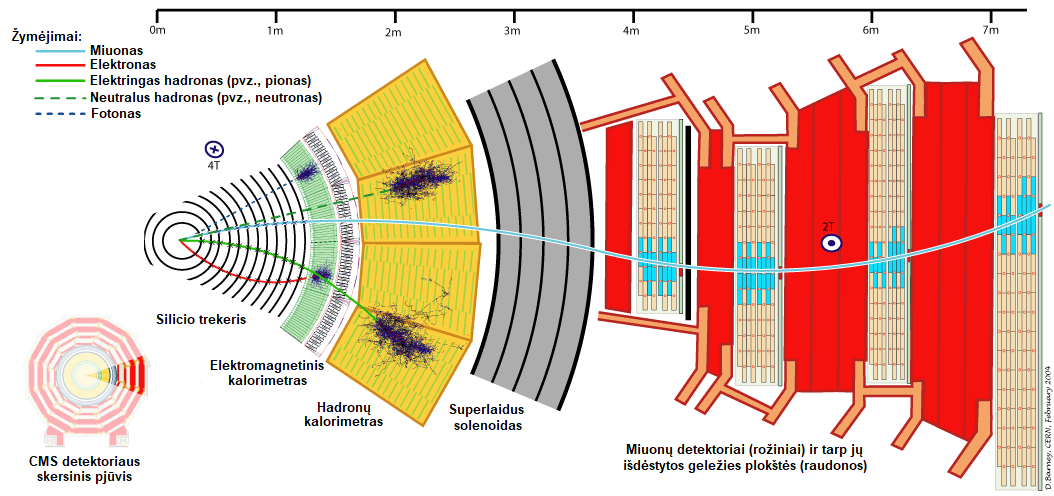
\includegraphics[width=\textwidth]{CMSslice_LT.png}
	\caption{\label{fig:CMSslice}Skersinis CMS detektoriaus pjūvis \cite{CMSslice}.
	Skirtingos linijos žymi įvairių dalelių, išlekiančių iš protonų susidūrimo vietos, trajektorijas.
	Trūki linija žymi elektriškai neutralios dalelės trajektoriją, kuri silicio trekų detektoriuje
	neužfiksuojama.}
\end{figure}

Arčiausiai protonų susidūrimo vietos yra išdėstytas trekų detektorius (angl.\ \textit{silicon tracker}),
pagamintas iš silicio pikselių ir juostelių.
Į nuskurdintą puslaidininkio sluoksnį pataikiusios elektringos dalelės išlaisvina krūvininkus, taip sugeneruodamos
elektrinį signalą.
Trekų detektorius turi daug plonų puslaidininkio sluoksnių, tad išanalizavus skirtinguose sluoksniuose užregistruotą
signalą galima nustatyti, kokia kryptimi nulėkė protonų susidūrimo metu sukurtos elektringosios dalelės.
Puslaidininkio sluoksniai padaryti kaip įmanoma plonesni, kad pralėkdama dalelė juose prarastų kuo mažiau energijos
ir nepakeistų savo trajektorijos.

Pralėkusios trekų detektorių, dalelės pirmiausia pataiko į elektromagnetinį kalorimetrą (angl.\ \textit{Electromagnetic Calorimeter} -- ECAL).
Šio subdetektoriaus paskirtis -- detektuoti elektronus ir fotonus bei išmatuoti jų energiją.
Elektromagnetinis kalorimetras pagamintas iš scintiliuojančios medžiagos -- švino volframato $\mathrm{PbWO}_{4}$.
Į elektromagnetinį kalorimetrą pataikius reliatyvistiniu greičiu lekiančiam elektronui, scintiliatoriaus medžiagos elektronai yra sužadinami
ir relaksuoja skleisdami šviesą.
Elektrono energija nustatoma išmatavus švytėjimo intensyvumą, kuris yra proporcingas elektrono prarastai energijai medžiagoje.
Elektronas kalorimetre yra visiškai sustabdomas.
Į tankią scintiliatoriaus medžiagą pataikę fotonai pavirsta į elektrono-pozitrono porą, kurios energija jau gali būti išmatuojama
tokiu pačiu būdu.
Ar signalas elektromagnetiniame kalorimetre yra susijęs su elektronu, ar su fotonu galima atskirti pagal tai, ar jis gali būti susietas su
trekų detektoriuje užregistruotais signalais.

Dalelės, kurios nėra sustabdomos elektromagnetiniame kalorimetre, pataiko į hadronų kalorimetrą (angl.\ \textit{hadron calorimeter} -- HCAL).
Šis subdetektorius sustabdo hadronus ir matuoja jų energiją.
Hadronų kalorimetre naudojamas plastiko scintiliatorius.
Kadangi hadronai yra gerokai sunkesni ir skvarbesni už elektronus, norint juos sustabdyti tarp scintiliatoriaus sluoksnių yra įterptos
vario plokštės, o taip pat šis subdetektorius yra gerokai storesnis už elektromagnetinį kalorimetrą.

Už hadronų kalorimetro yra sumontuotas iki superlaidumo temperatūros atšaldytas solenoidinis elektromagnetas.
Kai detektorius yra įjungtas, solenoidu teka maždaug $19.1$~kA stiprio elektros srovė, sukurianti iki $4$~T siekiantį magnetinį lauką.
Jo paskirtis -- iškreivinti krūvį turinčių dalelių trajektorijas.
Pagal tai, kuria kryptimi dalelės trajektorija užsisuka, galima nustatyti dalelės elektrinį krūvį,
o iš trajektorijos kreivumo spindulio galima įvertinti ir jos skersinį impulsą.
Jis taip pat leidžia atskirti miuonus nuo didelės energijos hadronų.
Vis dėlto, norint užtikrinti, kad kuo mažiau hadronų pasiektų tolimesnius detektoriaus sluoksnius, už
solenoido yra sumontuotas papildomas hadronų kalorimetro sluoksnis, vadinamas išoriniu hadronų kalorimetru
(angl.\ HCAL \textit{outer}).

Pačioje CMS detektoriaus išorėje keliais sluoksniais išdėstyti miuonų detektoriai.
Miuonai yra apie $200$ kartų sunkesni už elektronus, bei nesąveikauja stipriąja sąveika, todėl yra gerokai skvarbesni
už visas kitas detektuojamas daleles.
Dėl šios priežasties jie nėra sustabdomi nei elektromagnetiniame, nei hadronų kalorimetruose.
Miuonų detektoriai veikia dujų išlydžio principu -- bet kokia detektoriaus išorę pasiekusi elektringa dalelė jonizuoja
miuonų detektoriuose esančias dujas.
Per jonizuotas dujas pratekėjusi elektros srovė užfiksuojama kaip pataikymas.
Nors miuonų detektoriai galėtų registruoti bet kokių elektringų dalelių pataikymus, dažniausiai visos
kitos dalelės yra sustabdomos ankstesniuose detektoriaus sluoksniuose.
Tuo tarpu miuonai nėra sustabdomi net ir miuonų detektorių sistemoje -- dujiniai detektoriai tik užfiksuoja jų
trajektoriją.
Šių dalelių impulsas yra nustatomas iš trajektorijos kreivumo.
Kad impulsą būtų galima nustatyti kuo efektyviau, tarp miuonų detektorių yra sumontuotos geležinės magnetinio
lauko apgrąžos plokštės, kurios sustiprina magnetinį lauką miuonų detektoriuose, tuo pačiu neleisdamos jam tęstis toli
už detektoriaus ribų.
Taip pat šios plokštės užblokuoja kelią paskutinėms iki jų prasiskverbusioms dalelėms, kurios nėra miuonai
arba neutrinai.
Neutrinai yra vienintelės dalelės, kurios CMS detektoriumi nedetektuojamos.
Vis dėlto, neutrino pėdsaką galima nuspėti apskaičiavus visų užregistruotų dalelių skersinių impulsų vektorinę sumą
ir pastebėjus didelį skersinio impulso trūkumą tam tikra kryptimi: susiduriantys protonai juda išilgai $z$ ašies,
todėl visų susidariusių dalelių skersinių impulsų vektorinė suma turėtų būti lygi nuliui.

\subsection{Trigeriai}
Per kiekvieną protonų pluoštelių prasikeitimo įvykį (toliau juos vadinsime tiesiog įvykiais) CMS detektorius
užregistruoja apie $1$ MB informacijos.
Norint išsaugoti kiekvieną kas $25$~ns vykstantį įvykį reikėtų ypatingai greitos elektronikos, gebančios išrašyti
duomenis $\sim\!\!40$~TB/s greičiu, o taip pat ir nerealiai didelių duomenų saugyklų.
Vis dėlto, labai didelė šių įvykių dalis mokslininkams nėra įdomi -- tai nepakankamai energingi susidūrimai
arba labai dažnai vykstantys ir jau gerai ištirti procesai.
CMS eksperimente išsaugomų įvykių skaičiui sumažinti (stengiantis atmesti kiek įmanoma daugiau neįdomių ir palikti
kuo daugiau įdomių įvykių) naudojama dviejų lygių trigerių sistema, susidedanti iš pirmo lygio
(angl.\ \textit{level} 1 -- L1) ir aukšto lygio (angl.\ \textit{high-level trigger} -- HLT) trigerių \cite{CMStrig}.

Pirmojo lygio trigeris -- tai šalia detektoriaus sumontuota specialiai tam sukurta kompiuterinės įrangos sistema.
Ši sistema realiu laiku minimaliai apdoroja kalorimetrų bei miuonų detektorių duomenis ir atrenka įvykius, atsižvelgiant
į juose esančius fizikinių objektų kandidatus (signalas miuonų detektoriuose gali reikšti miuoną, signalai kalorimetruose --
elektroną, fotoną, hadronus, ženklus signalų detektoriuje trūkumas -- neutrinus).
Galutinis pirmo lygio trigerio atrankos etapas -- papildomų kriterijų, kurie gali būti pasirinkti iš programuojamo
kriterijų meniu, pritaikymas.
Šie papildomi kriterijai gali būti keičiami ir greitintuvui veikiant, priklausomai nuo jo veikimo sąlygų
(su greitintuvu dirbantys technikai kartais eksperimentuoja keisdami per vieną pluoštelių prasikeitimą susiduriančių protonų skaičių).
Kriterijus visada stengiamasi parinkti taip, kad juos praeitų ne daugiau kaip $10^5$ įvykių per sekundę
(tai yra CMS elektronikos pajėgumų viršutinė riba).
Papildomi kriterijai gali būti tokie: fizikinio objekto kandidato energija turi viršyti slenkstinę ribą, įvykyje turi
būti tam tikras objekto kandidatų skaičius, ir pan.
Pirmo lygio trigeris turi apytiksliai $4$~µs signalo užlaikymo intervalą, per kurį sistema nusprendžia, ar įvykis turėtų būti
išsaugomas tolimesnei analizei. 

Aukšto lygio trigeris -- tai programinės įrangos rinkinys, skirtas detaliau išanalizuoti pirmo lygio trigerį praėjusius
įvykius ir dar labiau sumažinti jų skaičių prieš įrašant ilgalaikiam saugojimui.
Aukšto lygio trigerio programinė įranga yra sudiegta į įprastus superkompiuterius, pastatytus netoli CMS detektoriaus.
Juose įvykio vaizdas atkuriamas pasinaudojant pilna detektoriaus užregistruota informacija, o atpažintiems fizikiniams
objektams, siekiant išsaugoti tik potencialiai įdomius įvykius, pritaikomi griežtesni atrankos kriterijai.
Aukšto lygio trigeris sumažinta išsaugomų duomenų kiekį iki maždaug $400$ įvykių per sekundę.
Šie įvykiai yra įrašomi ilgalaikiam saugojimui, kad vėliau galėtų būti analizuojami mokslininkų.

Neretai Didžiajame hadronų greitintuve protonų susidūrimų skaičius per vieną pluoštelių prasikeitimą padidinamas tiek,
kad net ir potencialiai įdomūs įvykiai įvyksta taip dažnai, kad jų visų tampa nebeįmanoma išsaugoti.
Tokiu atveju, tiek pirmo, tiek aukšto lygio trigeriuose gali būti panaudojamas nustatyto dydžio tarpavimas (angl.\ \textit{prescale}),
kuris atmeta fiksuotą porciją potencialiai įdomių įvykių.
Pavyzdžiui, dvejetui lygus tarpavimas sumažins išsaugomų potencialiai įdomių įvykių skaičių perpus.


\subsection{Protonų susidūrimo įvykių atkūrimas}
CMS detektoriaus užregistruoti signalai sujungiami į pilną protonų susidūrimo įvykio vaizdą, naudojantis
dalelių srauto (angl.\ \textit{Particle Flow} -- PF) algoritmu \cite{ParticleFlow}.
Šis algoritmas sujungia trekų detektoriuje užregistruotus signalus su pataikymais į kalorimetrus arba miuonų
detektorius, taip nustatydamas susidariusių dalelių tipus, jų trajektorijas bei kitus parametrus
(energiją, impulsą, elektrinį krūvį ir pan.).
Dalelių srautas gali atkurti ne tik dalelių trajektorijas, bet ir kitus fizikinius objektus, pavyzdžiui,
hadronų čiurkšles (ši sąvoka plačiau paaiškinta \ref{sec:jets} skyriuje) ar skersinio impulso trūkumą.

Dalelių srauto algoritmas įvykius atkuria iteratyviai.
Pirmiausia nustatomos \ltq{akivaizdžiausios} trajektorijos (pavyzdžiui, tokios, kurios susideda iš pataikymų
kiekviename trekų detektoriaus sluoksnyje, gerai sutampa su pataikymais į kalorimetrus ar miuonų detektorius,
kalorimetro išmatuota energija gerai sutinka su impulsu, nustatytu iš trajektorijos kreivumo ir pan.).
Tada signalai, kurie buvo panaudoti nustatant geriausias trajektorijas, pašalinami ir atkūrimo procedūra
kartojama su tuo, kas liko, tik šiek tiek sušvelninus trajektorijos nustatymo \ltq{gerumo} reikalavimus.
Iteracijos atliekamos, kol panaudojama visa detektoriaus užregistruota informacija.
Galų gale gaunamas platus galutinių įvykio produktų sąrašas, leidžiantis pamatyti pilną protonų susidūrimo įvykio vaizdą,
kurį jau gali analizuoti mokslinės tyrimų grupės.
Atkurto Drell-Yan proceso įvykio kandidato pavyzdys atvaizduotas \ref{fig:Event} paveiksle.
Įvykio vaizdas sugeneruotas naudojantis CMS programinės įrangos pakete esančia programa FireWorks.

Per kiekvieną protonų pluoštelių prasikeitimą įvyksta kelios dešimtys protonų susidūrimų, o taip pat, iki kol
visos susidariusios dalelės išlekia iš detektoriaus arba yra sustabdomos, jau būna prasidėjęs ir kitas pluoštelių
prasikeitimas (persiklojantys protonų susidūrimai angliškai vadinami \textit{pile-up} -- PU).
Iš kelių dešimčių vienu metu įvykusių protonų susidūrimų dažniausiai įdomus būna tik vienas (o įvykiuose, kurių
nepraleido trigeris, įdomaus nebuvo nei vieno).
Dalelių srauto algoritmas sugeba atskirti didžiąją dalį dalelių trajektorijų, susijusių su pašaliniais
protonų susidūrimais ir jas atmesti.
Iš tiesų, dalelių srauto algoritmas yra toks pajėgus, kad net geba atpažinti daleles, kurios atsirado kitų dalelių skilimo metu
ar susieti užregistruotus fotonus su elektronais, kurie juos išspinduliavo dėl judėjimo su pagreičiu magnetiniame lauke.
Norint sėkmingai taikyti tokį algoritmą svarbu, kad aktyvių detektoriaus elementų sudalinimas būtų pakankamai smulkus,
o pats detektorius būtų sandarus.
CMS detektorius gerai atitinka abu šiuos kriterijus.

\begin{figure}[t]
	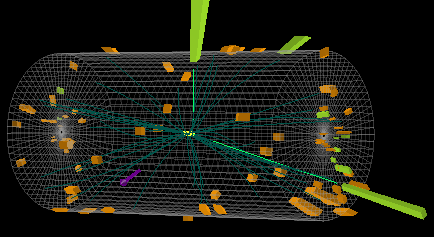
\includegraphics[width=0.8\textwidth]{Event.png}
	\caption{\label{fig:Event}
		Dalelių srauto algoritmu atkurto Drell-Yan proceso įvykio kandidato vaizdas.
		Tamsiai žalios linijos vaizduoja mažos energijos dalelių (daugiausia pionų) trajektorijas,
		o ryškios šviesiai žalios linijos -- didelės energijos elektronų trajektorijas.
		Šviesiai žali ir oranžiniai stulpeliai vaizduoja atitinkamai elektromagnetinio ir hadronų kalorimetro
		segmentuose užregistruotus energijos kiekius.
		Atkurtame įvykyje matomos elektronų poros invariantinė masė apytiksliai lygi $90$ GeV, t.y., labai artima $Z$ bozono masei.
	}
\end{figure}


\subsection{Signalas ir triukšmas}\label{sec:sig_bkg}
Drell-Yan proceso metu susidaro du priešingo elektrinio krūvio izoliuoti leptonai, neapsupti pašalinių dalelių.
Izoliuotų leptonų pora gali susidaryti ir kitų procesų metu.
Atskirai paėmus vieną detektoriaus užregistruotą įvykį neįmanoma vienareikšmiškai teigti, kad tai yra Drell-Yan
arba kito proceso įvykis.
Pašaliniai procesai, kurie dėl savo galutinių produktų panašumo trukdo tirti Drell-Yan procesą, vadinami triukšmo įvykiais.
Tuo tarpu Drell-Yan proceso įvykiai vadinami signalu.
Didžiajame hadronų greitintuve vykdomiems Drell-Yan proceso matavimams izoliuotų leptonų triukšmus sukuria šie procesai,
išdėstant juos tikėtinumo didėjimo tvarka:
\begin{itemize}
	\item Vieno viršūninio kvarko ir $W$ bozono vienalaikio susidarymo įvykiai ($tW$ arba $\tbarW$), kai tiek $W$ bozonas,
	tiek viršūninis kvarkas skyla leptoniškai
	\item Dviejų masyvių leptoniškai skylančių vektorinių bozonų įvykiai ($WW$, $\WZ$ ir $\ZZ$)	
	\item Viršūninio kvarko ir antikvarko poros ($\ttbar\,$) įvykiai, kai abu viršūniniai kvarkai skyla leptoniškai
	\item Drell-Yan proceso taonų kanalas ($\DYtau$), kai taonai skyla į lengvesnius leptonus
\end{itemize}
Yra žinoma, kad su $WW$, $\WZ$, $\ZZ$, $tW$, $\tbarW$ ir $\ttbar$ procesais susiję triukšmai yra svarbūs visoje invariantinės
masės srityje, tuo tarpu $\DYtau$ -- mažos invariantinės masės (maždaug $40-80$~GeV) srityje
\cite{DY_CMS2011, DY_CMS2013, DY_CMS2015, DY_CMS2019}.
Taip pat galimi triukšmo įvykiai, susiję su dalelių srauto algoritmo neteisingai atpažintais fizikiniais objektais.
Dažniausi tokio tipo triukšmai siejasi su čiurkšlėmis, kurios buvo klaidingai atpažintos kaip izoliuoti leptonai.
Apie šiuos triukšmus plačiau rašoma \ref{sec:jets} skyriuje.

Matuojant Drell-Yan proceso diferencialinį reakcijos skerspjūvį stengiamasi tiriamą fazinę erdvę apriboti taip, kad būtų
atmetama kiek įmanoma daugiau triukšmo įvykių, tuo pačiu išsaugant kuo didesnį signalo įvykių skaičių.
Vis dėlto, net į apribotą tyrimo sritį patenka reikšmingas triukšmo įvykių skaičius.
Šį įvykių skaičių reikia įvertinti kaip įmanoma tiksliau ir jį atmesti iš tiriamų pasiskirstymų.

\subsection{Su čiurkšlėmis susiję triukšmo įvykiai}\label{sec:jets}
Protonų susidūrimuose galutinė proceso būsena (angl.\ \textit{final state} -- taip vadinamas išeinančių dalelių rinkinys
procesą aprašančioje Feinmano diagramoje -- reakcijos produktas) dažnai yra palydima vieno ar kelių kvarkų ir/arba gliuonų
(jeigu neskaičiuojame likusių partonų, kurie nesusąveikauja ir nulekia apytiksliai tiesiai).
Pavyzdžiui, energingą kvarką arba gliuoną prieš sąveikaudami gali išspinduliuoti reakcijoje dalyvaujantys partonai.
Įvykio metu sukurtos masyvios dalelės (taonai, $W$, $Z$ ir Higso bozonai) su tam tikra tikimybe taip pat gali skilti į kvarkus.
Vis dėlto, izoliuotų kvarkų arba gliuonų dalelių detektoriais aptikti neįmanoma.

Daug energijos turintys kvarkai ją praranda spinduliuodami gliuonus.
Tuo tarpu gliuonai gali skilti į kvarko ir antikvarko poras arba patys spinduliuoti papildomus gliuonus.
Tokiu būdu iš vieno galutinės būsenos partono pagaminamas \ltq{partonų dušas} (angl.\ \textit{parton shower}).
Kai partonų duše esančių dalelių energija pasidaro pakankamai maža, stipriosios sąveikos konstanta išauga
tiek, kad perturbatyvus kvantinės chromodinamikos aprašymas nustoja galioti.
Žemose energijose ($<\!1$~GeV) pasireiškia kvarkų \ltq{įkalinimas} (angl.\ \textit{confinement}): dėl sąveikos stiprumo
kvarkai gali egzistuoti tik grupėse, kuriose jų spalvinis krūvis neutralizuojamas.
Šiame režime bandant kvarkus vieną nuo kito atitraukti reikėtų tiek energijos, kad jos užtektų iš vakuumo pagaminti
naujai kvarko-antikvarko porai, kuri suformuotų naujas grupes su atitrauktaisiais kvarkais ir neutralizuotų jų spalvinį krūvį.
Dėl šio reiškinio partonų duše lekiantys kvarkai ir gliuonai pradeda formuoti hadronus.
Tai vadinama hadronizacija.
Jos metu hadronų pagaminama labai daug, tad vieno energingo partono pėdsaką detektorius užregistruoja kaip besiplečiančio
kūgio formos dalelių srautą, sudarytą iš daugybės įvairių rūšių hadronų bei kitų dalelių \cite{Jets}.
Šie dalelių srautai vadinami čiurkšlėmis (angl.\ \textit{jets}).

Čiurkšlėse dažniausiai susidaro ne tik hadronai.
Pavyzdžiui, čiurkšlėse galimas nemažas skaičius fotonų, kurie atsiranda daugiausia iš neutralaus piono skilimų.
Taip pat vykstant didelės energijos partonų sklaidos procesams galima sukurti sunkiųjų kvarkų, kurie gyvuoja trumpai
ir skildami gali pagaminti leptonų.
Pavyzdžiui, elektronas arba miuonas yra randamas apytiksliai $20\%$ gelminio kvarko sukurtų čiurkšlių
(angl.\ \textit{b-jets}) ir apytiksliai $10\%$ žaviojo kvarko sukurtų čiurkšlių (angl.\ \textit{c-jets}) \cite{LeptonJets}.
Čiurkšlėse susidariusios stipriąja sąveika nesąveikaujančios dalelės neretai pagelbėja nustatant,
kokį kvarką atitinka matoma čiurkšlė.
Vis dėlto, jos kartais gali ir suklaidinti -- retais atvejais čiurkšlės yra supainiojamos su protonų susidūrimo metu
pagamintu leptonu
\cite{DY_CMS2011, DY_CMS2013, DY_ATLAS2013, DY_ATLAS2014, DY_CMS2015, DY_ATLAS2016, DY_ATLAS2017, DY_CMS2019, EleID, MuonID}.

Bendru atveju čiurkšlėse susidarę leptonai nėra izoliuoti -- jie yra apsupti hadronų srauto.
Vis dėlto, pasitaiko atvejų, kai leptonas yra pakankamai energingas, kad susumuotas greta lėkusių hadronų ir fotonų
skersinis impulsas yra gerokai mažesnis už leptono skersinį impulsą (tai gali sudaryti įspūdį, kad leptonas yra izoliuotas).
Taip pat galimi atvejai, kai didesnę dalį čiurkšlės energijos nešasi vienas ar keli fotonai.
Įvykio atkūrimo algoritmui klaidingai susiejus trekų detektoriuje užfiksuotą trajektoriją su fotonų paliktu signalu
elektromagnetiniame kalorimetre, čiurkšlę galima neteisingai atkurti kaip elektrono objektą.
Jeigu išmatuota tokio \ltq{netikro} elektrono energija yra gerokai didesnė už jį supančių hadronų energiją, galima jį
klaidingai palaikyti izoliuotu.
Labai retais atvejais nutinka ir taip, kai energinga čiurkšlė pralekia hadronų kalorimetrą ir palieka signalą miuonų
detektoriuje (toks procesas angliškai vadinamas \textit{hadronic punchthrough}).
Jeigu \ltq{netikro} miuono trajektorija dalelių srauto algoritmo yra atkuriama kaip ganėtinai tiesi (o tai reiškia
didelį skersinį impulsą), įmanoma netgi klaidingai pagalvoti, kad jis yra izoliuotas.
Prie klaidingo čiurkšlių atpažinimo gali prisidėti ir neidealus detektoriaus bei trajektorijų atkūrimo efektyvumas
(nebūtinai bus užfiksuotos visos čiurkšlėje susidariusios dalelės).

Pagrindiniai su klaidingai atpažintomis čiurkšlėmis susiję Drell-Yan proceso triukšmo įvykiai yra $W$ bozono ir vienos čiurkšlės
įvykiai ($\WJets$) bei stipriosios sąveikos nulemti kelių čiurkšlių įvykiai (sutrumpintai žymimi $\QCD$).
Yra žinoma, kad miuonų kanale su čiurkšlėmis susiję triukšmai turi reikšmingą indėlį žemos invariantinės masės,
o elektronų kanale -- visoje invariantinės masės srityje \cite{DY_CMS2011, DY_CMS2013, DY_CMS2015, DY_CMS2019}.
Tiriant Drell-Yan procesą, į šių triukšmo procesų indėlį taip pat svarbu atsižvelgti.

\subsection{Triukšmo įvykių skaičiaus įvertinimas}
Turint detektoriaus išmatuotų duomenų rinkinį neįmanoma vienareikšmiškai pasakyti, kurie įvykiai yra susiję su triukšmo
procesais.
Įmanoma tik ribotu tikslumu įvertinti, koks skaičius triukšmo įvykių galėjo patekti į tiriamą rinkinį.
Triukšmo įvykių skaičius įvertinamas pasinaudojant papildomais duomenų rinkiniais, kurie gali būti gauti iš tikro matavimo
arba sumodeliuoti.

Grubų triukšmo įvykių skaičiaus įvertį galima gauti pasinaudojus Monte Carlo (MC) metodu sumodeliuotais protonų susidūrimo įvykiais.
Įvykių modeliavimas būna atliekamas keliais lygmenimis.
Pirmiausia sumodeliuojamas pats protonų susidūrimas ir gaunama, kokios dalelės susidarė jo metu.
Tada modeliuojami po susidūrimo vykstantys antriniai procesai, tokie, kaip hadronizacija, spinduliavimas, dalelių skilimai bei
tuo pačiu metu vykstantys pašaliniai protonų susidūrimai.
Galiausiai modeliuojama, kaip įvykio produktai sąveikauja su medžiaga -- detektoriaus komponentais.
Tokį virtualų eksperimentą kartojant daug kartų galima gauti vidutinį rezultatą, kuris yra palyginamas su realiu eksperimentu.

Vis dėlto, sumodeliuoti įvykius taip, kad virtualaus eksperimento sąlygos idealiai atitiktų realaus eksperimento sąlygas,
yra praktiškai neįmanoma.
Atsižvelgiant į kai kuriuos neatitikimus modeliuotiems įvykiams gali būti pritaikomos CMS eksperimento mokslinių grupių
rekomenduojamos pataisos.
Tačiau vis tiek egzistuoja modeliavimo neapibrėžtumų, kurie kenkia įverčio kokybei (pavyzdžiui, nepakankamos žinios apie
atskirų triukšmo procesų įvykių tikėtinumus, neidealus detektoriaus atsako modeliavimas, papildomi protonų susidūrimai ir pan.).
Blogiausiai modeliavimas įvertina procesus, kurių tikėtinumas labai didelis, o įvykių atrankos praėjimo efektyvumas labai
mažas -- norint gauti tolydų ir tikrovišką pasiskirstymą reikėtų tokių įvykių sumodeliuoti nepaprastai daug, o tam
reikalingi neįmanomai dideli skaičiavimo ir duomenų saugojimo resursai.
Būtent tokie yra su klaidingai atpažintomis čiurkšlėmis susiję $\WJets$ ir $\QCD$ procesai -- jų tikėtinumas didesnis už
Drell-Yan proceso (atitinkamai $3$ ir net $500$ kartų), o tikimybė čiurkšlei būti klaidingai atpažintai kaip analizei
atrinktam leptonui yra ganėtinai maža. 
Dėl šių trūkumų naudoti vien modeliuotus duomenis yra vengiama ir, kur įmanoma, stengiamasi triukšmo įvykių skaičių
įvertinti naudojant matavimu grįstus metodus.

Matavimu grįsti (angl.\ \textit{data-driven}) metodai apjungia matavimą ir modeliavimą, kad būtų gautas kuo
tikroviškesnis įvykių skaičiaus įvertis.
Šių metodų veikimo principas remiasi signalo ir kontrolinės sričių apibrėžimais.
Signalo sritis pasirenkama taip, kad į ją patektų kuo daugiau signalo ir kuo mažiau triukšmo įvykių -- tai yra pagrindinė
tyrimo sritis.
Kontrolinė sritis pasirenkama taip, kad į ją patektų kuo daugiau triukšmo ir kuo mažiau signalo įvykių.
Sritys gali būti apibrėžiamos įvairiais užregistruotus įvykius apibūdinančių parametrų apribojimais, pavyzdžiui,
apribojant tam tikrų įvykyje užregistruotų dalelių ar kitų fizikinių objektų skaičių, tiriamų dalelių trajektorijų izoliuotumą, jų
elektrinius krūvius ir pan.
Signalo ir kontrolinė sritys turi būti nepersidengiančios.
Matavimu grįsti metodai nustato sąsają tarp triukšmo įvykių pasiskirstymo signalo ir kontrolinėje srityje.
Tada triukšmo įvykių skaičius, apskaičiuotas kontrolinėje srityje, ekstrapoliuojamas į signalo sritį.
Šiais laikais atliekamuose Drell-Yan proceso diferencialinio reakcijos skerspjūvio matavimuose populiarūs yra šie matavimu
grįsti metodai: $\emu$ metodas \cite{DY_CMS2011, DY_CMS2013, DY_ATLAS2014, DY_CMS2015, DY_CMS2019},
ABCD metodas \cite{DY_CMS2011, DY_CMS2013, DY_ATLAS2014, DY_CMS2015, DY_ATLAS2016, DY_ATLAS2017},
klaidingo atpažinimo metodas \cite{DY_CMS2011, DY_CMS2013, DY_ATLAS2013, DY_CMS2015, DY_ATLAS2016, DY_CMS2019}.
Jei triukšmo įvykyje susidaro dvi nestabilios dalelės, kurios gali skilti į izoliuotus leptonus nepriklausomai
(tokį aprašymą atitinka $tW$, $\tbarW$, $WW$, $\ttbar\,$ ir $\DYtau$ procesai), jo indėlis gali būti įvertintas $\emu$ metodu.
Įvykiams, susijusiems su klaidingai atpažintomis čiurkšlėmis, įvertinti gali būti naudojami klaidingo atpažinimo ir ABCD metodai.
Toliau šiame darbe bus gilinamasi į klaidingo atpažinimo metodą.


\subsection{Klaidingo atpažinimo metodas}\label{sec:FR}
Klaidingo atpažinimo metodas yra ganėtinai populiarus nustatant triukšmo įvykių skaičių, kuriuose viena ar kelios čiurkšlės
buvo klaidingai atpažintos kaip izoliuoti leptonai.
Nemažas skaičius CMS ir ATLAS eksperimentuose vykdomų leptono-antileptono galutinės būsenos tyrimų (daugiausia tai yra
Drell-Yan proceso tyrimai arba naujų didelės masės bozonų paieška) vienaip ar kitaip šį metodą naudoja
\cite{DY_CMS2011, DY_CMS2013, DY_ATLAS2013, DY_CMS2015, DY_ATLAS2016, DY_CMS2019, Z'_ATLAS2011, Z'_CMS2011, Z'_CMS2012,
Z'_CMS2013, Z'_ATLAS2014, Z'_CMS2015, Z'_CMS2017, Z'_CMS2018}.
Vis dėlto, daugelyje viešai prieinamų straipsnių klaidingo atpažinimo teorinis veikimo principas nėra aprašytas, arba tai padaryta
labai minimaliai.
Ypatingai CMS kolektyvo straipsniuose daugiau koncentruojamasi į praktinius klaidingo atpažinimo metodo aspektus.
Nepaisant to, galima susidaryti bendrą įspūdį, kad klaidingo atpažinimo metodo taikymas susideda iš dviejų dalių:
pirmiausia įvertinama klaidingo atpažinimo tikimybė, o tada gauta tikimybės vertė panaudojama kaip svorinis
daugiklis įvykiams, kurie nepraėjo pagrindinės tyrimo atrankos.

Įprastai klaidingo atpažinimo tikimybė yra įvertinama pasinaudojant duomenų rinkiniu, gaunamu smarkiai atlaisvinus
tyrimui naudojamus atrankos kriterijus.
Šis duomenų rinkinys apdorojamas taip, kad jame liktų vien tik klaidingai kaip leptonai atpažintos čiurkšlės.
Tada skaičiuojama, kokia dalis klaidingai atpažintų čiurkšlių patenka į tiriamąją (signalo) sritį
\cite{DY_ATLAS2016, Z'_ATLAS2011, Z'_CMS2011, Z'_ATLAS2014, Z'_CMS2015}.
Gautas santykis yra vadinamas klaidingo atpažinimo tikimybe.
Toliau ją žymėsime raide $f$.
Klaidingo atpažinimo tikimybė dažniausiai matuojama kaip funkcija nuo kelių parametrų.
Įvertinta tikimybė pritaikoma įvertinant, kiek su klaidingai atpažintomis čiurkšlėmis susijusių įvykių
galėjo praeiti dviejų leptonų įvykių atranką.
Tam pasinaudojama įvykių rinkiniais, kuriuose vienas arba abu leptonai nepraėjo signalo atrankos kriterijų, ir
šiems įvykiams klaidingo atpažinimo tikimybė pritaikoma kaip svorinis daugiklis \cite{Z'_ATLAS2011, Z'_CMS2011, Z'_CMS2015}.
Įvykio svoris susideda iš daugiklio $f/(1-f)$ kiekvienam objektui, kuris nepraėjo signalo atrankos (t.y., visas įvykio svoris
susideda iš vieno arba dviejų tokių daugiklių) \cite{Z'_CMS2015}.
Šie svoriai transformuoja įvykių pasiskirstymą, kuriuose leptonus imituojančios čiurkšlės praėjo tik atlaisvintą leptono atranką,
bet nepraėjo signalo sritį atitinkančios atrankos, į pasiskirstymą, atitinkantį įvykius, kuriuose leptonus imituojančios čiurkšlės
praėjo signalo atranką.

Kai kurios tyrimų grupės klaidingo atpažinimo tikimybės pritaikymą aprašo kiek kitaip \cite{DY_ATLAS2016, Z'_ATLAS2014}.
Jeigu įvertiname ne tik tikimybę klaidingai atpažintai čiurkšlei patekti į signalo sritį, bet ir tikimybę \ltq{tikram}
elektronui patekti į signalo sritį (angl.\ \textit{acceptance}, toliau šį dydį žymėsime raide $a$), galime gauti lygčių sistemą,
susiejančią įvykius su \ltq{tikrais} arba \ltq{netikrais} leptonais ir detektoriaus registruojamus įvykius su objektais signalo
arba kontrolinėje srityse:

\begin{align}
\label{eq:FRmatrix}
	\begin{bmatrix}
		N_{SS} \\		
		N_{SC} \\
		N_{CS} \\
		N_{CC} \\
	\end{bmatrix}
	=
	\begin{bmatrix}
		a_1a_2 & a_1f_2 & f_1a_2 & f_1f_2 \\
		a_1(1-a_2) & a_1(1-f_2) & f_1(1-a_2) & f_1(1-f_2) \\
		(1-a_1)a_2 & (1-a_1)f_2 & (1-f_1)a_2 & (1-f_1)f_2 \\
		(1-a_1)(1-a_2) & (1-a_1)(1-f_2) & (1-f_1)(1-a_2) & (1-f_1)(1-f_2) \\
	\end{bmatrix}
	=
	\begin{bmatrix}
		N_{RR} \\
		N_{RF} \\
		N_{FR} \\
		N_{FF} \\
	\end{bmatrix}
	\! ,
\end{align}
čia $N$ žymi įvykių skaičių, indeksai $S$ ir $C$ -- atitinkamai leptono objektą, patenkantį į signalo arba kontrolinę sritį,
o indeksai $R$ ir $F$ -- atitinkamai tikrą ir netikrą leptonus.
Detektorius išmatuoja įvykių skaičius $N_{SS}$, $N_{SC}$ ir t.t., o tyrėjus iš tikrųjų dominantys dydžiai $N_{RF}$, $N_{FR}$ ir
$N_{FF}$ (įvykiai su klaidingai atpažintomis čiurkšlėmis) gali būti gauti invertavus \eqref{eq:FRmatrix} išraiškoje esančią matricą.
Toks triukšmo įvykių skaičiaus įvertinimo būdas kartais dar vadinamas matricų metodu.

Taigi, nors klaidingo atpažinimo metodas viešai prieinamoje literatūroje nėra labai išsamiai aprašytas, susidaro įspūdis, jog
jo įgyvendinimas nėra vienareikšmis: jis gali turėti nemažai variacijų ir konkreti metodika turi būti adaptuota atliekamam tyrimui.
Klaidingo atpažinimo tikimybės ir su čiurkšlėmis susijusių triukšmo įvykių skaičiaus įverčiai tarp skirtingų tyrimų bendru atveju neturi
sutapti, nes tiek klaidingo atpažinimo tikimybė, tiek triukšmo įvertis gan smarkiai priklauso nuo analizėje taikomų atrankos kriterijų,
kontrolinės srities apibrėžimo ir pan.
Naudojantis surinkta informacija, labai apibendrintą klaidingo atpažinimo metodo teorinį veikimo principą pateikiame žemiau.

Sakykime, kad esant integruotam šviesiui $\Lumi$ pagaminama $N_{jet}$ čiurkšlių.
Jeigu tikimybė čiurkšlei būti klaidingai atpažintai kaip tam tikros rūšies leptonui yra $f_0$, iš viso bus klaidingai atpažinta
$N_{fake}=f_0 N_{jet}$ čiurkšlių.
Drell-Yan proceso tyrime leptonams taikomi papildomi atrankos reikalavimai, siekiant, kad atranką praeitų kuo
mažiau klaidingai atpažintų objektų.
Sakykime, kad tikimybė klaidingai atpažintai čiurkšlei praeiti šiuos reikalavimus lygi $f$.
Tada iš viso turėsime $N_{pass \,\&\, fake}=ff_0 N_{jet}$ čiurkšlių, kurios gali praeiti analizėje taikomus leptono
atrankos reikalavimus.
Tikimybę $f_0$ eksperimentiškai įvertinti yra sudėtinga, bet taikant klaidingo atpažinimo metodą ji išsiprastina ir lieka
įvertinti tikimybę, kad klaidingai atpažintos čiurkšlės pateks į signalo sritį, t.y., rasti $f$.
Ją apskaičiuojame taip:
\begin{equation}
\label{eq:FRtheor}
	f = \frac{N_{pass \,\&\, fake}}{N_{fake}} .
\end{equation}
Taigi, pagrindine užduotimi nustatant klaidingo atpažinimo tikimybę yra skaičių $N_{fake}$ bei $N_{pass \,\&\, fake}$ įvertinimas.
Tai galima padaryti skirtingais metodais, kurių daugelis įvairiais būdais kombinuoja matavimą ir modeliavimą.

Vykdant Drell-Yan proceso įvykių atranką ieškoma dviejų numatytus kriterijus atitinkančių leptonų.
Taigi, klaidingai atpažinti gali būti nulis, vienas arba abu leptonai.
Pilną atranką praėjusių įvykių skaičių galime išreikšti taip (tą galime išsivesti iš \eqref{eq:FRmatrix} išraiškos):
\begin{equation}
\label{eq:2passSeparated}
	N_{SS} = N_{RR} a_1 a_2 + N_{RF} a_1f_2 + N_{FR} f_1a_2 + N_{FF} f_1 f_2 \; ,
\end{equation}
čia $N_{SS}$ -- įvykių su dviem atranką praėjusiais leptonais skaičius, $N_{RR}$ -- įvykių su dviem tikrais
leptonais skaičius, $N_{RF}$ ir $N_{FR}$ -- įvykių su vienu tikru leptonu ir viena klaidingai atpažinta čiurkšle skaičius,
$N_{FF}$ -- įvykių su dviem klaidingai
atpažintomis čiurkšlėmis skaičius.
Čia nekreipiame dėmesio į fizikinio objekto atpažinimo efektyvumą.
Paprastumo dėlei, apjunkime dėmenis $N_{RF}$ ir $N_{FR}$ po vienu skaičiumi $N_{RF+FR}$:
\begin{equation}
	N_{RF} a_1f_2 + N_{FR} f_1a_2 \equiv N_{RF\!+\!FR}\,af \, , 
\end{equation}
čia dešinėje pusėje numetėme indeksus nuo $a$ ir $f$, su sąlyga, kad žinome, kuri dalelė įvykyje tikras, o kuri -- netikras
leptonas ir taikome daugiklius $a$ ir $f$ atitinkamai tikram ir netikram leptonui.
Tai leidžia \eqref{eq:2passSeparated} išraišką sutrumpinti taip:
\begin{equation}
\label{eq:2pass}
	N_{SS} = N_{RR} a_1 a_2 + N_{RF\!+\!FR}\, af + N_{FF} f_1 f_2 \; .
\end{equation}
Panašūs sutrumpinimai bus naudojami ir toliau.
Klaidingo atpažinimo metodo tikslas -- nustatyti \eqref{eq:2pass} išraiškoje esančius antrąjį ir trečiąjį dėmenis.
Tai padaroma suskaičiuojant įvykius, kuriuose klaidingai atpažinta čiurkšlė \textbf{nepraėjo} leptono atrankos kriterijų
(tikimybė jų nepraeiti lygi $1\!-\!f$).
Pavyzdžiui, įvykius su vienu atrankos nepraėjusiu leptonu (nesvarbu, kuriuo) galime išreikšti taip:
\begin{equation}
	\label{eq:1fail}
	\begin{gathered}
		N_{SC\!+\!CS} = N_{RR} \left( a_1(1-a_2) + (1-a_1)a_2 \right) + N_{RF\!+\!FR} \left( a(1-f) + (1-a)f \right) + \\
			   + N_{FF} \left( f_1(1-f_2) + (1-f_1)f_2 \right).
	\end{gathered}
\end{equation}
Išsireiškiame $N_{RF\!+\!FR}$:
\begin{equation}
\label{eq:realfake}
	N_{RF\!+\!FR} = \frac{ N_{SC\!+\!CS} - N_{RR} (a_1(1-a_2)+(1-a_1)a_2) - N_{FF} (f_1(1-f_2)+(1-f_1)f_2) }
				   { (a(1-f)+(1-a)f) }.
\end{equation}
Jeigu $a$ yra ganėtinai didelis ($\approx \!1$), o $f$ -- ganėtinai mažas ($\approx \!0$), \eqref{eq:realfake} išraišką galima
supaprastinti, vardiklyje esantį dėmenį $(1-a)f$ atmetant kaip mažą dydį.
Dėmenį $N_{RR} \left( a_1(1-a_2) + (1-a_1)a_2 \right)$ galime rasti iš modeliavimo, o $N_{FF} (f_1(1-f_2)+(1-f_1)f_2)$ -- pasinaudodami
įvykiais, kuriuose dvi klaidingai atpažintos čiurkšlės nepraėjo leptono atrankos kriterijų.
Iš tiesų:
\begin{equation}
\label{eq:FRWjets}
	N_{SC\!+\!CS} - N_{RR} \left( a_1(1-a_2) + (1-a_1)a_2 \right) - N_{FF} \left(f_1(1-f_2)+(1-f_1)f_2 \right) \approx N_{SC\!+\!CS}^{\WJets} \; ,
\end{equation}
nes iš įvykių, kuriuose vienas fizikinis objektas nepraeina atrankos, atmetus visus įvykius, kuriuose dalyvauja du tikri elektronai
arba dvi klaidingai atpažintos čiurkšlės, liekame su įvykiais, kuriuose buvo vienas tikras leptonas ir viena klaidingai atpažinta
čiurkšlė, o dominuojantis tokio tipo procesas yra $\WJets$.
Galime supaprastinti \eqref{eq:realfake} išraišką:
\begin{equation}
\label{eq:realfakeSimple}
	N_{RF\!+\!FR} = \frac{ N_{SC\!+\!CS}^{\WJets} }
				   		 { (a(1-f)+(1-a)f) }.
\end{equation}
Įvykius su dviem atrankos nepraėjusiais leptonais galime išreikšti taip:
\begin{equation}
\label{eq:2fail}
	\begin{gathered}
		N_{CC} = N_{RR} (1-a_1)(1-a_2) + N_{RF\!+\!FR} (1-a)(1-f) + 
						+ N_{FF} (1-f_1)(1-f_2).
	\end{gathered}
\end{equation}
Išsireiškiame $N_{FF}$:
\begin{equation}
\label{eq:2fake}
	N_{FF} = \frac{ N_{CC} - N_{RR} (1-a_1)(1-a_2) - N_{RF\!+\!FR} (1-a)(1-f) }
					 { (1-f_1)(1-f_2) },
\end{equation}
čia dėmenis $N_{RR} (1-a_1)(1-a_2)$ ir $N_{RF\!+\!FR} (1-a)(1-f)$ galime rasti iš modeliavimo.
Panašiai, kaip su $\WJets$ \eqref{eq:FRWjets} išraiškoje, čia galime užrašyti:
\begin{equation}
\label{eq:FRQCD}
	N_{CC} - N_{RR} (1-a_1)(1-a_2) - N_{RF\!+\!FR} (1-a)(1-f) \approx N_{CC}^{\QCD} \; ,
\end{equation}
nes dominuojantis procesas, kuriame dalyvauja dvi klaidingai atpažintos čiurkšlės yra $\QCD$.
Taigi, \eqref{eq:2fake} išraišką galime sutrumpintai užrašyti taip:
\begin{equation}
\label{eq:2fakeSimple}
	N_{FF} = \frac{ N_{CC}^{\QCD} }
				  { (1-f_1)(1-f_2) },
\end{equation}
Įstatę išvestas išraiškas į \eqref{eq:2pass} gauname:
\begin{equation}
\label{eq:2passFR}
	\begin{gathered}
		N_{SS} = N_{RR} a_1 a_2 + \frac{N_{SC\!+\!CS}^{\WJets}}{(a(1-f)+(1-a)f)}af +
				    \frac{N_{CC}^{\QCD}}{(1-f_1)(1-f_2)}f_1f_2 \approx \\ \approx
					N_{RR} a_1 a_2 + N_{SC\!+\!CS}^{\WJets} \frac{f}{1-f} +
					N_{CC}^{\QCD} \frac{f_1 f_2}{(1-f_1)(1-f_2)}, 
	\end{gathered}
\end{equation}
čia $(1-a)f$ atmetėme kaip mažą dydį.
Taigi, norint įvertinti su klaidingai atpažintomis čiurkšlėmis susijusių triukšmo įvykių skaičių signalo srityje,
turime nustatyti, kiek buvo tokių triukšmo įvykių, kuriuose klaidingai atpažintos čiurkšlės nepraėjo atrankos
kriterijų ir kiekvienam atrankos nepraėjusiam objektui pritaikyti daugiklį $f/(1-f)$.


\newpage
\section{Drell-Yan proceso tyrimo metodika}
Šiame skyriuje supažindinama su atlikto darbo metodika: trumpai pristatomi naudoti duomenų rinkiniai bei programinė įranga,
supažindinama su vykdyta protonų susidūrimo įvykių atrankos procedūra bei atrinktiems įvykiams pritaikytomis pataisomis.
Toliau paaiškinama, kaip buvo matuojamos klaidingo atpažinimo tikimybės bei kaip jos buvo panaudotos gaunant su klaidingai
atpažintomis čiurkšlėmis susijusių triukšmo įvykių skaičiaus įverčius. Galiausiai supažindinama su rezultato neapibrėžtumų
įvertinimo principais.


\subsection{Duomenų rinkiniai ir analizės kodai}\label{sec:data}
Darbui atlikti buvo naudojami CERN CMS detektoriaus užregistruoti protonų susidūrimų duomenys.
Duomenys buvo surinkti 2016 metais, esant $13$~TeV susidūrimų energijai.
Jų kiekis atitinka $35.9$~\invfb integruotą šviesį ($\sim\!2 \cdot 10^{15}$ protonų susidūrimų).
Tai yra $\sim\!10$ kartų daugiau įvykių, nei užregistruota $2015$-aisiais metais \cite{DY_CMS2019}.
CMS detektoriaus užfiksuoti įvykiai yra suskirstomi į duomenų rinkinius grupuojant pagal tai,
kiek ir kokio tipo objektų juose buvo aptikta.
Skirtingi duomenų rinkiniai gali būti persidengiantys (turėti tų pačių įvykių).
Šiame darbe buvo naudojami trys skirtingi duomenų rinkiniai:
1) įvykių su bent vienu užfiksuotu miuonu rinkinys (\ttt{SingleMuon}),
2) įvykių su bent dviem elektromagnetiniais objektais (elektronais arba fotonais) rinkinys (\ttt{DoubleEG}),
3) įvykių su bent vienu fotonu rinkinys (\ttt{SinglePhoton}).
Naudoti duomenų rinkiniai buvo dalinai apdoroti CMS Drell-Yan tyrimo mokslinės grupės.

Detektoriaus duomenų interpretavimui buvo pasitelkiami modeliuoti Drell-Yan proceso bei svarbiausių triukšmo
procesų duomenų rinkiniai.
Drell-Yan proceso bei $W$ bozono ir čiurkšlės ($\WJets$) įvykiai buvo sumodeliuoti su
\textsc{MadGraph5\_aMC@NLO} \cite{MG_aMCatNLO}.
Ši programa įvykius modeliuoja antros eilės (NLO) kvantinės chromodinamikos perturbacijų tikslumu.
Viršūninio kvarko ir antikvarko poros ($t\bar{t}\,$) bei vieno viršūninio kvarko ir $W$ bozono ($tW$ arba
$\tbarW$) procesai buvo sumodeliuoti naudojant \textsc{Powheg} įvykių modeliavimo programą \cite{powheg_ttbar, powheg_tW}.
Vieno fotono ir vienos čiurkšlės ($\gJets$) įvykiai buvo sumodeliuoti su programa \textsc{Sherpa} \cite{Sherpa}.
\textsc{Powheg} ir \textsc{Sherpa} įvykius modeliuoja antros eilės (NLO) perturbacijų tikslumu.
Dviejų bozonų procesų ($WW$, $\WZ$, $\ZZ$) bei kelių čiurkšlių ($\QCD$) proceso modeliavimas buvo atliktas su
\textsc{Pythia8} \cite{pythia82}.
\textsc{Pythia8} įvykius modeliuoja pirmos eilės (LO) tikslumu.
Visi antriniai procesai (kvarkų ir gliuonų hadronizacija, papildomų dalelių
spinduliavimas, nestabilių dalelių skilimai, pašaliniai tuo pačiu metu vykstantys protonų susidūrimai ir pan.)
buvo sumodeliuoti su \textsc{Pythia8}.
Dalelių sąveika su CMS detektoriaus medžiaga buvo sumodeliuota su \textsc{Geant4} programa
\cite{geant4}.
Modeliuoti skirtingų procesų įvykių rinkiniai yra nepersidengiantys.
Sumodeliuotų procesų reakcijos skerspjūviai pateikiami \ref{table:Xsec} lentelėje.
Joje taip pat pateikiamas tikėtinas kiekvieno proceso įvykių skaičius, kai integruotas šviesis lygus $35.9$~\invfb.

\begin{table}[t!]
	\begin{tabular}{|c|c|c|}
		\hline
		Procesas & Reakcijos skerspjūvis (pb) & Tikėtinas įvykių skaičius \\ 
		\hline\hline
		$\mathrm{DY} \!\!\rightarrow\! ll$ & $2.39\times 10^4$ & $8.58\times 10^8$ \\ %23908.693
		\hline		
		$\ZZ$ & $16.52$ & $5.93\times 10^5$ \\
		\hline
		$tW$ & $35.85$ & $1.29\times 10^6$ \\
		\hline
		$\tbarW$ & $35.85$ & $1.29\times 10^6$ \\
		\hline
		$\WZ$ & $47.13$ & $1.69\times 10^6$ \\
		\hline
		$WW$ & $118.70$ & $4.26\times 10^6$ \\
		\hline	
		$\ttbar$ & $831.76$ & $2.98\times 10^7$ \\
		\hline	
		$\WJets$ & $6.15\times 10^4$ & $2.21\times 10^9$ \\ %61526.70
		\hline
		$\gJets$ & $1.39 \times 10^5$ & $4.98\times 10^9$ \\
		\hline
		$\QCD$ ($\mu$) & $9.01\times 10^6$ & $3.23\times 10^{11}$ \\
		\hline
		$\QCD$ (EM) & $1.86\times 10^7$ & $6.67\times 10^{11}$ \\
		\hline
	\end{tabular}
	\caption{\label{table:Xsec} Tyrime naudotų modeliuotų duomenų rinkinių reakcijų skerspjūviai ir tikėtini įvykių skaičiai, kai integruotas
	šviesis lygus $35.9$~\invfb. Žymėjimai $\QCD$ ($\mu$) ir $\QCD$ (EM) reiškia įvykių rinkinius, \ltq{praturtintus}
	atitinkamai miuonais arba elektromagnetiniais objektais (bent vienoje iš čiurkšlių susiformuoja miuonas arba fotonai/elektronai).}
\end{table}

Darbe naudoti duomenys yra saugomi Pietų Korėjos Kyungpook nacionalinio universiteto Tier2 duomenų centre.
Duomenų apimtis siekia apie $20$ TB.
Duomenims analizuoti buvo rašomi programiniai moduliai C++ kalba.
Parašyti programiniai moduliai buvo leidžiami CERN duomenų analizei skirtoje ROOT aplinkoje \cite{ROOTarticle}.
Duomenų analizė buvo išskaidyta į du etapus.
Pirmiausia Seulo nacionalinio universiteto CERN Tier3 skaičiavimo centre buvo atliekama darbui svarbių įvykių atranka.
Atranka buvo vykdoma pagal kriterijus, aptariamus \ref{sec:selection} skyriuje, paleidus kodus nuotoliniu būdu.
Atrinkti įvykiai buvo įrašomi į naujus duomenų failus ir toliau analizuojami atsisiuntus į vietinį kompiuterį.
Atsisiųsti duomenų rinkiniai užima apie $66$ GB, didžiąją dalį jų apimties sudaro klaidingo atpažinimo tikimybės matavimui
naudoti duomenys.
Programinio kodo versijų sekimui ir tvarkymui buvo naudojama \textit{Github} versijų valdymo sistema.
Visi parašyti C++ programiniai moduliai yra patalpinti viešoje \textit{Github} saugykloje, esančioje adresu
\url{https://github.com/marijusambrozas/DrellYan2016/tree/master/SelectedX}.


\begin{table}[t!]
	\begin{tabular}{|c|c|c|}
		\hline
		\multirow{2}{9em}{\centering\textbf{Kriterijaus tipas}} & \multirow{2}{13em}{\centering\textbf{\textit{ee} atrankos reikalavimas}} &
			\multirow{2}{12em}{\centering\textbf{\textit{µµ} atrankos reikalavimas}}\\
		 & & \\
		\hline\hline
		\multirow{4}{9em}{\centering Aukšto lygio trigeris} & \multirow{4}{12em}{\centering\ttt{HLT\_Ele23Ele12}} &
			\multirow{2}{13em}{\centering\ttt{HLT\_IsoMu24} arba \ttt{HLT\_IsoTkMu24}} \\
		 & & \\ \cline{3-3}
		 & & \multirow{2}{12em}{\centering Bent vienas miuonas turi būti aktyvavęs trigerį} \\
		 & & \\
		\hline\hline
		\multirow{4}{9em}{\centering Kinematiniai reikalavimai} &
			\multirow{2}{13em}{\centering $p_{\mathrm{T \, 1}} > 28$~GeV, $p_{\mathrm{T \, 2}} > 17$~GeV} &
			\multirow{2}{12em}{\centering $p_{\mathrm{T \, 1}} > 28$~GeV, $p_{\mathrm{T \, 2}} > 17$~GeV} \\
		 & & \\ \cline{2-3}
		 & $|\eta_{\mathrm{SC}}| < 2.4$, & \multirow{2}{12em}{\centering $|\eta| < 2.4$} \\
		 & išskyrus $1.4442<|\eta_{\mathrm{SC}}|<1.566$ & \\
		\hline\hline
		\multirow{2}{9em}{\centering Dalelės atpažinimo reikalavimai} & \multirow{2}{13em}{\centering \ltq{\ttt{MediumID}} reikalavimai} &
			\ltq{\ttt{TightID}} reikalavimai \\ \cline{3-3}
		 & & $I_{\mathrm{PF}}^{\mathrm{rel.}}<0.15$ \\
		\hline\hline
		\multirow{7}{9em}{\centering Reikalavimai geresniam signalo išskyrimui} &
			\multirow{7}{13em}{\centering Atrankos reikalavimus turi atitikti lygiai 2 elektronai} &
			\multirow{4}{12em}{\centering Pasirenkami 2 miuonai, kuriuos galima tiksliausiai suvesti į vieną pirminę viršūnę su $\chi^2<20$} \\
		 & & \\
		 & & \\
		 & & \\ \cline{3-3}
		 & & Priešingi elektriniai krūviai \\ \cline{3-3}
		 & & \multirow{2}{12em}{\centering Plokštuminis kampas $\alpha < (\pi - 0.005)$~rad} \\
		 & & \\
		\hline
	\end{tabular}
	\caption{\label{table:selection}Apibendrinti Drell-Yan proceso įvykių kandidatų atrankos kriterijai.
	Indeksai $1$ ir $2$ žymi atitinkamai greitesnįjį ir lėtesnįjį leptoną.
	$\eta_{\mathrm{SC}}$ žymi elektromagnetinio kalorimetro segmento, į kurį pataikė elektronas, pseudospartą.}
\end{table}

\subsection{Drell-Yan proceso įvykių atranka}\label{sec:selection}
Ne visi CMS detektoriaus užfiksuoti protonų susidūrimo įvykiai yra tinkami Drell-Yan proceso fizikinei analizei.
Norint iš $2016$ metais CMS užregistruotų duomenų išskirti dominančią informaciją, reikėjo įvykdyti įvykių atranką pagal
numatytus specialius kriterijus.
Atrankos kriterijai yra apibendrinti \ref{table:selection} lentelėje.
Jie buvo parinkti taip, kad atranką praeitų kuo didesnis skaičius Drell-Yan signalo įvykių ir būtų atmetama kuo daugiau
triukšmo įvykių, ypač tų, kurie susiję su klaidingai atpažintais fizikiniais objektais.

Elektronų kanalo įvykiams buvo naudojamas aukšto lygio dviejų elektronų trigeris, kuris aktyvuojamas užregistravus vieną elektroną
su skersiniu impulsu, didesniu nei $23$~GeV ir kitą -- su skersiniu impulsu, viršijančiu $12$~GeV.
Siekiant, kad tyrimo sritis būtų kuo mažiau paveikta ženkliai mažesnių už vienetą įvykių registravimo efektyvumų, ji buvo papildomai
apribojama reikalaujant, kad vieno elektrono skersinis impulsas viršytų $28$~GeV, o kito -- $17$~GeV.
Impulso apribojimai parinkti atsižvelgiant į trigerio ypatumus: naudotas trigeris turėtų aktyvuotis aptikus elektronus
su skersiniais impulsais, viršijančiais $(23, 12)$~GeV, tačiau jis maksimalų savo veikimo efektyvumą pasiekia prie šiek
tiek aukštesnių skersinio impulso verčių.
Taigi, kriterijus su slenksčiu $(28, 17)$~GeV užtikrina, kad būtų atrinkti įvykiai, kuriuose trigerio efektyvumas yra
įsisotinęs.
Taip pat buvo reikalaujama, kad elektromagnetinio kalorimetro elementų, į kuriuos elektronai pataikė, pseudospartos koordinatės
($\eta\equiv -\mathrm{ln}\left[\tan\left(\theta/2\right)\right]$, kur $\theta$ -- kampas tarp dalelės trajektorijos ir $z$ ašies)
absoliutinė vertė neviršytų $2.4$ bei nepatektų į sritį $1.4442<|\eta|<1.566$, kurioje yra perėjimas tarp kalorimetro
cilindrinės ir antgalių dalies.
Pseudospartos apribojimai skirti atmesti sritis, kuriose elektromagnetinio kalorimetro veikimo efektyvumas ne toks
aukštas.

Norint užtikrinti, kad nagrinėjamame įvykių rinkinyje būtų kuo mažiau klaidingai atpažintų čiurkšlių arba elektronų,
atsiradusių fotonui pavirtus į elektrono-pozitrono porą, kiekvienam elektronui buvo taikomas CMS elektrono ir fotono
fizikinių objektų mokslinės grupės (CMS \textit{EGamma Physics Object Group}) rekomenduojamas vidutiniškai griežtų
elektrono atpažinimo kriterijų rinkinys \ltq{\ttt{MediumID}} (panašaus tipo reikalavimai, skirti analizuoti senesnių
metų CMS detektoriaus duomenims, yra viešai prieinami išspausdintame straipsnyje \cite{EleID}, o naujesni kriterijai,
kurie buvo taikomi šioje analizėje, yra prieinami tik CMS vidiniuose dokumentuose ir šiame darbe pridedami 2 priede).
Šiuos kriterijus turėtų atitikti apie $80\%$ tikrų elektronų ir apie $3\%$ klaidingai atpažintų objektų \cite{EleID}.
Nors Drell-Yan proceso metu turėtų atsirasti priešingo krūvio elektronų pora, atrenkant įvykius elektronams priešingo
krūvio reikalavimai nebuvo taikomi dėl ganėtinai didelės tikimybės, kad elektrono krūvis bus neteisingai atpažintas
(ji siekia apie $1.5\%$ \cite{EleID}).
Vietoje to, buvo reikalaujama, kad įvykyje būtų užfiksuoti lygiai du vidutiniškai griežtus kriterijus atitinkantys
elektronai.

Miuonų kanalo įvykiams buvo naudojamas aukšto lygio vieno miuono trigeris, kuris aktyvuojamas aptikus bent vieną izoliuotą
miuoną, kurio skersinis impulsas viršija $24$~GeV.
Miuonas turi būti atpažintas pasinaudojant trekų detektoriaus ir miuonų detektorių informacija.
Taip pat buvo reikalaujama, kad bent vienas iš įvykyje užfiksuotų miuonų savo trajektorijos koordinatėmis sutaptų su signalu,
aktyvavusiu trigerį.
Toliau miuonų skersinis impulsas buvo apribojamas taip pat, kaip ir elektronų, siekiant užtikrinti, kad ir miuonų įvykiai
būtų atrinkti iš srities, kurioje trigerio efektyvumas yra įsisotinęs.
CMS išorėje esančių miuonų detektorių veikimo efektyvumas mažai priklauso nuo pseudospartos, todėl miuonų pseudospartai
buvo taikomas vienintelis apribojimas, kad jos absoliutinė vertė neviršytų $2.4$ (didesnių pseudospartos verčių
miuonų detektoriai neuždengia).
Norint atmesti miuonus, atsiradusius iš antrinių procesų bei netikrus miuonų signalus, atsiradusius iš miuonų detektorius
pasiekusių čiurkšlių, buvo taikomi CMS miuono fizikinių objektų mokslinės grupės (CMS \textit{Muon Physics Object Group})
rekomenduojamas labai griežtų miuono atpažinimo kriterijų rinkinys \ltq{\ttt{TightID}} \cite{MuonID}.
Šiuos kriterijus atitinka apie $95\%$ tikrų izoliuotų miuonų ir vos $0.3\%$ netikrų arba neizoliuotų miuonų.

Siekiant dar labiau sumažinti atranką praeinančių netikrų miuonų skaičių, kiekvienam labai griežtus reikalavimus
atitinkančiam miuonui papildomai buvo taikomas trajektorijos izoliuotumo reikalavimas: dalelių srauto algoritmo
apskaičiuotas trajektorijos santykinio izoliuotumo parametras negali viršyti $0.15$.
Santykinio izoliuotumo parametras $I^{\mathrm{rel.}}_{\mathrm{PF}}$ skaičiuojamas taip \cite{ParticleFlow}:
\begin{equation}
	\label{eq:isolation}
	I^{\mathrm{rel.}}_{\mathrm{PF}} = \frac{1}{p_{\mathrm{T}}} 
	\left( \sum_{\Delta R<0.3} p_{\mathrm{T}}^{\mathrm{hadron^{\pm}}} +
	\sum_{\Delta R<0.3} p_{\mathrm{T}}^{\mathrm{hadron^0}} + 
	\sum_{\Delta R<0.3} p_{\mathrm{T}}^{\gamma} \right) \; \mathrm{,}
\end{equation}
čia $\pT$ -- nagrinėjamo miuono skersinis impulsas, $\Delta R = \sqrt{\Delta \phi^{2} + \Delta \eta^{2}}$ -- kūgio,
brėžiamo aplink nagrinėjamo miuono trajektoriją, plotis, $p_{\mathrm{T}}^{\mathrm{hadron^{\pm}}}$ -- į nubrėžtą
kūgį patenkančių elektringų hadronų skersiniai impulsai, $p_{\mathrm{T}}^{\mathrm{hadron^0}}$ -- elektriškai neutralių
hadronų skersiniai impulsai,  $p_{\mathrm{T}}^{\gamma}$ -- fotonų skersiniai impulsai.
Įvykiai, kuriuose nėra bent dviejų miuonų, atitinkančių labai griežtus atpažinimo kriterijus bei papildomus izoliuotumo
reikalavimus, buvo iškart atmetami.
Likusiuose įvykiuose buvo bandoma išrinkti du miuonus, kurių krūviai yra priešingi ir kuriuos eitų pakankamai tiksliai
suvesti į vieną pirminę viršūnę: prie detektoriuje užfiksuotų pataikymų priderinus dvi iš vieno taško išeinančias kreives,
priderinimo gerumą nusakantis dydis $\chi^2$, tenkantis vienam laisvės laipsniui, turėtų neviršyti $20$.
Viename įvykyje pasitaikius kelioms tokius reikalavimus atitinkančioms miuonų poroms, iš jų buvo išsirenkama ta, kurios
$\chi^2$ yra mažiausias.
Labai retais atvejais reliatyvistiniai kosminiai miuonai gali pasiekti CMS detektorių ir imituoti miuono-antimiuono porą
(jeigu pralekia pro detektoriaus centrą), tad siekiant tokio triukšmo išvengti buvo pritaikytas papildomas kriterijus,
reikalaujantis, kad plokštuminis kampas tarp dviejų miuonų trajektorijų neviršytų $\pi-0.005$~rad.

Pagrindinis šiame darbe matuojamas dydis buvo atranką praėjusių leptonų porų invariantinė masė.
Kiekvienos leptonų poros invariantinė masė buvo supildoma į masių histogramą.
Tyrinėta masių sritis nuo $15$ iki $3000$~GeV.
Histogramos elektronų ir miuonų kanalams buvo brėžiamos atskirai.

\subsection{Modeliuotų įvykių skaičiaus normavimas}
Modeliuoti protonų susidūrimai buvo naudojami interpretuojant CMS detektoriaus duomenis bei įvertinant triukšmo įvykių
skaičių klaidingo atpažinimo metodu.
Eksperimento metu užfiksuotų įvykių skaičius priklauso nuo integruoto šviesio ir vykstančių procesų reakcijų skerspjūvių:
$N = \sigma\Lumi$.
Integruotas šviesis priklauso nuo dalelių greitintuvą valdančių eksperimentatorių pasirinkimų, tokių, kaip duomenų rinkimo laikas,
protonų susidūrimų dažnis, protonų pluoštelio matmenys ir tankis, pluoštelių prasikeitimo kampas ir pan.
Modeliuotų įvykių skaičius nuo tokių parametrų nepriklauso.
Teoriškai jų galima sumodeliuoti tiek, kiek tyrėjai pageidauja, tačiau dažniausiai šį skaičių apriboja turimi skaičiavimo
resursai -- stengiamasi, kad sumodeliuoti duomenys neužimtų per daug vietos ir jų analizė neužtruktų labai ilgai.
Bendru atveju modeliuotų įvykių skaičius nesutampa su eksperimente užregistruotu įvykių skaičiumi.

Norint išmatuotus pasiskirstymus palyginti su modeliuotais, būtina sumodeliuotą įvykių skaičių sunormuoti į eksperimento
metu pasiektą integruotą šviesį.
Tai padaroma kiekvienam modeliuotam įvykiui priskiriant svorinį daugiklį $\omega_{i}^{\mathrm{Norm.}}$.
T.y., pildant įvykių histogramą $i$-asis modeliuotas įvykis į ją yra įvedamas ne kaip vienas įvykis, o kaip
$\omega_{i}^{\mathrm{Norm.}}$ įvykio.
Svorinio daugiklio vertė gaunama pagal proporciją tarp tikėtino eksperimento metu užregistruotų įvykių skaičiaus $N$ ir
sumodeliuoto įvykių skaičiaus $N_{\mathrm{MC}}$:
\begin{equation}
	\label{eq:LOweight}
	\omega_{i}^{\mathrm{Norm.}} = \frac{ \sigma\Lumi }{ N_{\mathrm{MC}} } \; .
\end{equation}

Programos, kurios modeliuoja įvykius aukštesniu negu pirmos eilės (LO) perturbacijų tikslumu, pačios gali jiems priskirti
nelygius vienetui svorius -- svoriniai daugikliai atsiranda kaip perturbatyvios pataisos pirmos eilės tikslumu gautam
pasiskirstymui.
Todėl, norint sunormuoti aukštesnių eilių tikslumu sumodeliuotus įvykius, reikia atsižvelgti ne tik į jų skaičių, bet
ir kiekvienam įvykiui modeliavimo programos priskirtus svorius.
Taigi, aukštesnių eilių perturbacijų tikslumu sumodeliuotiems įvykiams svorinius daugiklius apskaičiuojame taip:
\begin{equation}
	\omega_{i}^{\mathrm{Norm.}} = \omega_{i}^{\mathrm{Gen.}} \frac{ \sigma\Lumi }{ \sum_{j=1}^{N}\omega_{j}^{\mathrm{Gen.}} } \; ,
	\label{eq:NLOweight}
\end{equation}
čia $\omega_{i}^{\mathrm{Gen.}}$ kiekvieno įvykio individualus svoris, priskirtas įvykių modeliavimo programos.
Ši išraiška nuo \eqref{eq:LOweight} skiriasi tuo, kad tikėtiną įvykių skaičių papildomai padauginame iš modeliavimo programos
priskirto svorio, o daliname ne iš sumodeliuotų įvykių skaičiaus, bet iš įvykių svorių sumos (ji atitinka didesniu tikslumu
įvertintą įvykių skaičių).
Matome, kad visus modeliavimo programos priskiriamus svorius pakeitus į vienetą (pirmos eilės tikslumo atvejis), \eqref{eq:LOweight}
ir \eqref{eq:NLOweight} išraiškos tampa vienodos.
Daugumai procesų $\omega_{i}^{\mathrm{Norm.}}<1$.
Šis dydis gali įgyti tiek teigiamas, tiek neigiamas vertes.


\subsection{Pataisos}\label{sec:corrections}
Modeliuojant protonų susidūrimus reikia atsižvelgti į labai didelį skaičių eksperimento parametrų, tokių, kaip protonų
susidūrimo vieta detektoriuje, pašalinių protonų susidūrimų skaičius (kuris priklauso nuo įvairių protonų pluoštelio parametrų),
skirtingų detektoriaus komponentų efektyvumai ir daug kitų.
Natūralu, kad modeliuoti įvykiai visų realaus eksperimento sąlygų idealiai neatkartos.
Siekiant atsižvelgti į reikšmingiausius neatitikimus, įvairios CMS mokslinės grupės rekomenduoja pataisas, kurias
pritaikius galima pagerinti sutapimą tarp eksperimento ir modeliavimo.

Elektronų poros invariantinės masės matavimo kokybei didelę įtaką daro elektronų energijos matavimo tikslumas,
o miuonų poros atveju -- jų skersinio impulso matavimo tikslumas.
Siekiant pagerinti invariantinės masės matavimo kokybę, visiems detektoriaus užregistruotiems elektrono objektams
buvo pritaikytos CMS elektrono ir fotono fizikinių objektų mokslinės grupės rekomenduojamos energijos matavimo
skalės pataisos.
Analogiškai miuonams buvo pritaikytos CMS Ročesterio mokslinės grupės pateikiamos miuonų impulso matavimo skalės
pataisos \cite{RocCorr}.
Šios pataisos buvo pritaikytos tiek CMS detektoriaus, tiek modeliuotiems įvykiams kaip pataisos daugikliai atitinkamai
elektrono energijai arba miuono skersiniam impulsui.
Šių daugiklių vertės išmatuotiems ir sumodeliuotiems įvykiams yra skirtingos.

2016 metais kiekvieno protonų pluoštelių prasikeitimo CMS detektoriuje metu įvykdavo vidutiniškai 23 protonų
susidūrimai \cite{CMSLumi}.
Vienu metu vykstančių protonų susidūrimų skaičius nulemia vidutinį įvykio metu susidarančių dalelių skaičių.
Užfiksuoto įvykio vaizdo atkūrimo kokybė gan smarkiai priklauso nuo dalelių trekų skaičiaus, tad lyginant
eksperimentą su modeliavimu svarbu gerai atkartoti pašalinius protonų susidūrimus.
Vis dėlto, dažnu atveju sumodeliuotas pašalinių protonų susidūrimų skaičiaus tikimybinis pasiskirstymas
nesutampa su eksperimentiniu.
Atsitiktinės susidūrimų fliuktuacijos šį nesutapimą nulemia tik iš dalies.
Didesnę įtaką jam turi Didžiojo hadronų greitintuvo technikų tyrinėjimai keičiant protonų spindulio intensyvumą,
pluoštelių formą, jų persiklojimo tūrį ir pan.

Nesutapimą tarp išmatuoto ir modeliuoto protonų susidūrimų skaičiaus pasiskirstymo bandoma sumažinti taikant
CMS šviesio fizikinių objektų grupės (CMS \textit{Luminosity Physics Object Group}) rekomenduojamas protonų
susidūrimo skaičiaus pataisas.
Kiekvienam modeliuotam įvykiui buvo priskiriamas papildomas svorinis daugiklis atsižvelgiant į jame buvusį protonų
susidūrimų skaičių.
Pataisa pritaikyta padarius prielaidą, kad vidutinis protonų susidūrimo skerspjūvis greitintuve yra lygus $64$~mb,
kai susidūrimų energija yra $13$~TeV.
Išmatuoti ir sumodeliuoti įvykyje atkurtų pirminių viršūnių (atitinkančių protonų susidūrimus) skaičiaus pasiskirstymai
prieš ir po pataisos elektronų poros įvykiuose palyginami \ref{fig:PUba}~pav.
Pirminių viršūnių skaičiaus pasiskirstymai miuonų poros įvykiams atrodo analogiškai, todėl nepateikiami.
Čia ir toliau paveikslų apatinėse dalyse pateikiami eksperimentinio ir modeliuoto rezultatų santykio grafikai.
Pritaikius pataisą, $10$-$30$ pirminių viršūnių skaičiaus srityje, kurioje yra $\sim\!91\%$ visų įvykių,
eksperimentinis ir modeliuotas pasiskirstymai pradėjo sutapti labai gerai -- skirtumas neviršija $9\%$.

\begin{figure}[t!]
	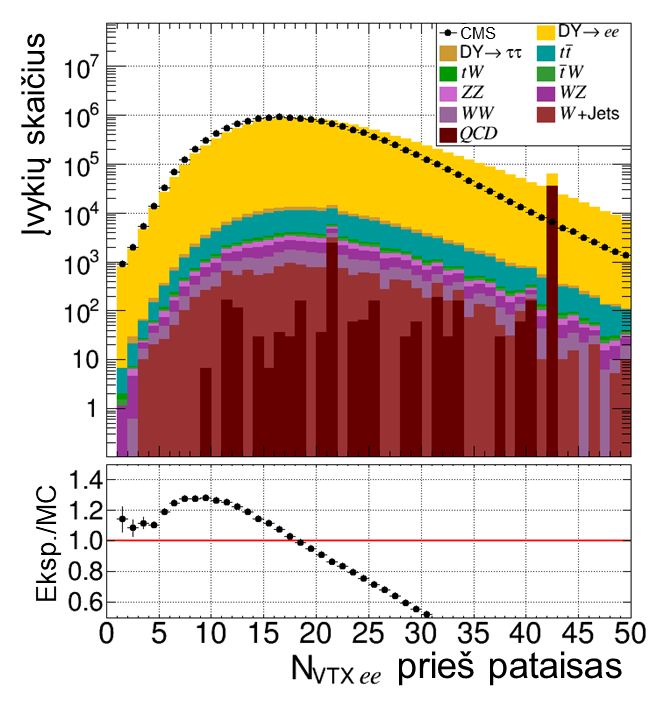
\includegraphics[width=0.48\textwidth]{Magistrinis/ee_nVTX_before.png}
	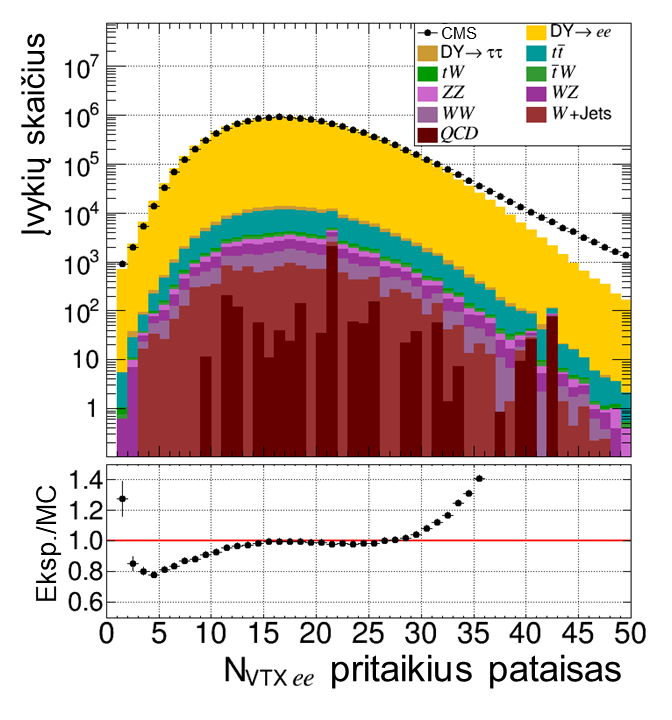
\includegraphics[width=0.48\textwidth]{Magistrinis/ee_nVTX_after.png}
	\vspace{-0.6cm}
	\caption{\label{fig:PUba} Pirminių viršūnių skaičiaus pasiskirstymai atranką praėjusiuose elektronų poros įvykiuose
		prieš (kairėje) ir po (dešinėje) pašalinių protonų susidūrimų skaičiaus pataisos pritaikymo.
		Juodi taškai vaizduoja CMS detektoriumi išmatuotą, o spalvoti stulpeliai -- modeliuotus pasiskirstymus.}
\end{figure}

Labai dažnai modeliavimas neteisingai imituoja realios eksperimentinės įrangos veikimo efektyvumus.
Kaip taisytini buvo išskiriami trigerių suveikimo efektyvumai, leptono trajektorijos atkūrimo ir dalelės teisingo
atpažinimo efektyvumai.
Miuonams papildomai buvo įskaitomas nesutapimas tarp tikro ir modeliuoto miuono izoliuotumo nustatymo efektyvumo.
Nesutapimai buvo taisomi modeliuotiems įvykiams pritaikius svorinius daugiklius $\prod_k(\epsilon_k^{\mathrm{Data}}/\epsilon_k^{\mathrm{MC}})$, 
kur raidės $\epsilon$ žymi efektyvumus, indeksai $k$ -- išskirtus eksperimento procesus (trigerio suveikimą ir t.t.),
o indeksai \ltq{MC} ir \ltq{Data} pažymi atitinkamai modeliuotą ir išmatuotą efektyvumus.
Efektyvumai yra patvirtinti CMS elektrono ir fotono bei miuono fizikinių objektų mokslinių grupių.
Svorinių daugiklių vertės buvo parametrizuojamos pagal įvykyje užregistruotų leptonų skersinius impulsus ir pseudospartas.
Tipinės svorinio daugiklio vertės siekė $\sim\!0.9$.
Miuonų poros invariantinės masės pasiskirstymai prieš ir po efektyvumų pataisų pritaikymo yra palyginti \ref{fig:invMba_mumu}~pav.,
o elektronų poros -- \ref{fig:invMba_ee} pav.
Efektyvumų pataisos padėjo pagerinti sutapimą tarp eksperimento ir modeliavimo vidutiniškai $10\%$.

\begin{figure}[t!]
	\RawFloats
	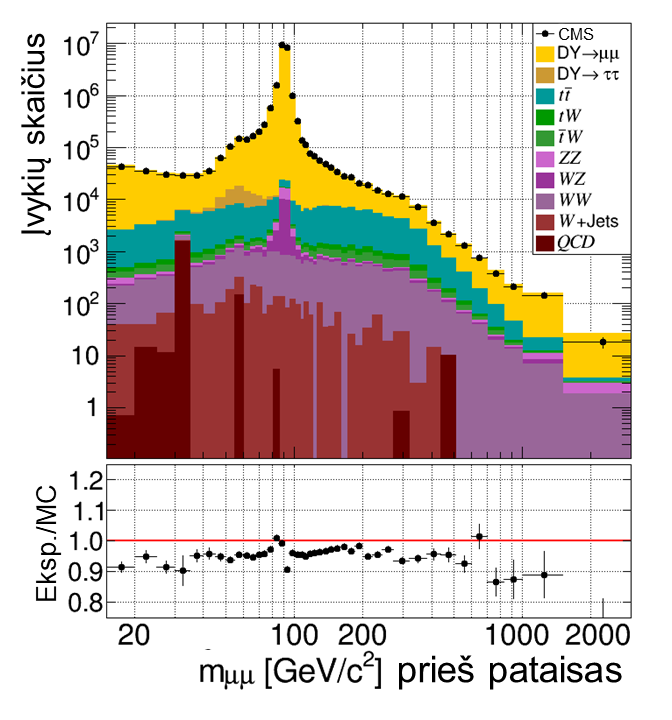
\includegraphics[width=0.48\textwidth]{Magistrinis/mumu_mass_before.png}
	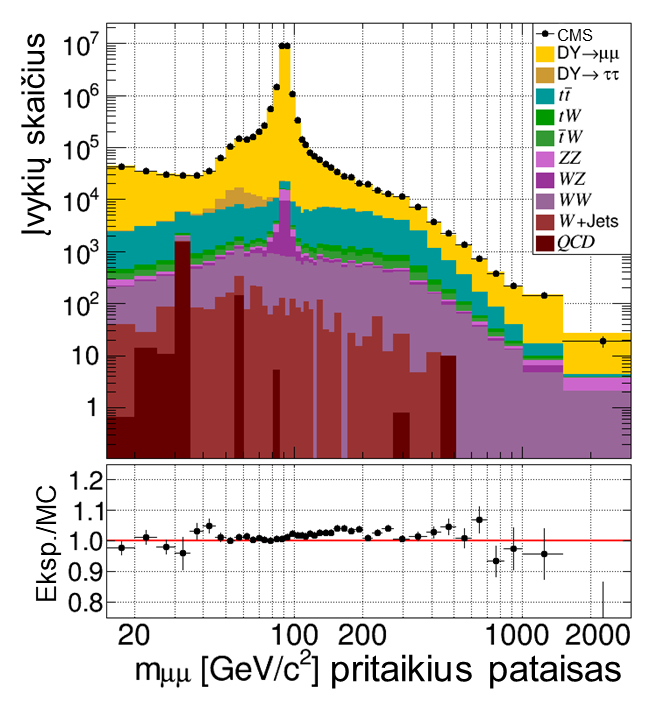
\includegraphics[width=0.48\textwidth]{Magistrinis/mumu_mass_after.png}
	\vspace{-0.6cm}
	\caption{\label{fig:invMba_mumu} Miuonų porų invariantinės masės pasiskirstymai prieš (kairėje) ir po (dešinėje)
	miuonų impulso matavimo skalės bei efektyvumo pataisų pritaikymo.}
	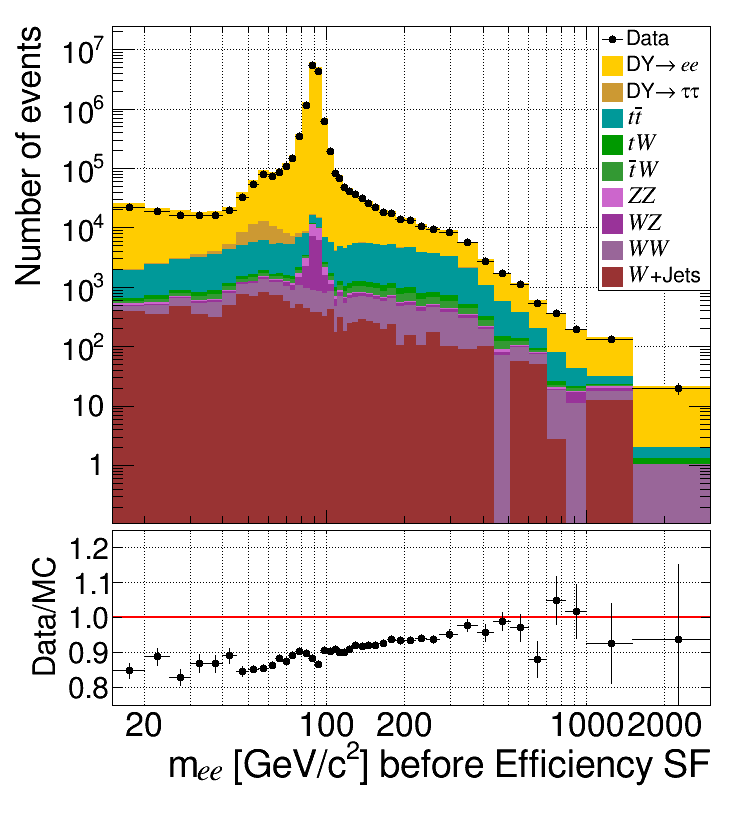
\includegraphics[width=0.48\textwidth]{Magistrinis/ee_mass_before.png}
	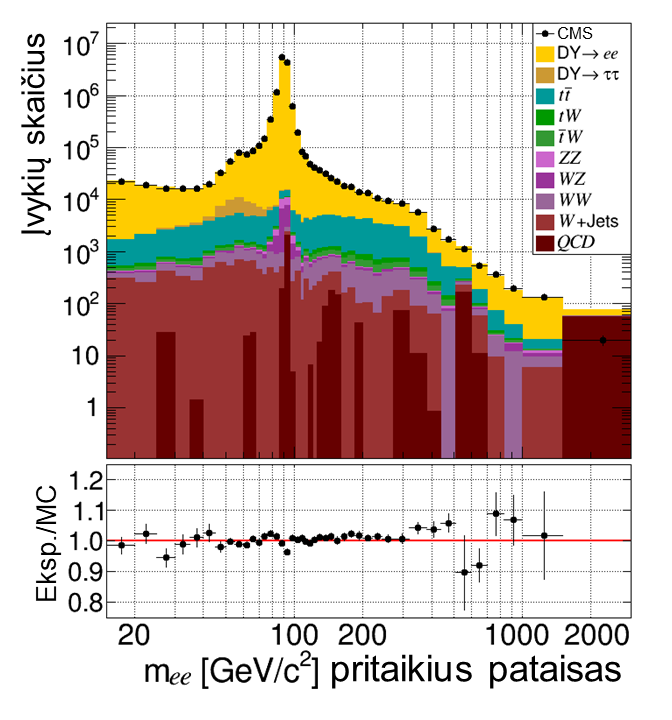
\includegraphics[width=0.48\textwidth]{Magistrinis/ee_mass_after.png}
	\vspace{-0.6cm}
	\caption{\label{fig:invMba_ee} Elektronų porų invariantinės masės pasiskirstymai prieš (kairėje) ir po (dešinėje)
	efektyvumo pataisų pritaikymo.}
\end{figure}

Matavimo ir modeliavimo rezultatų sutapimą gali paveikti ne vien modeliavimo trūkumai, bet taip pat ir neidealios
eksperimentinės sąlygos arba net eksperimentatorių klaidos.
Leptonų poros spartos pasiskirstymus reikšmingai paveikė dvi aplinkybės, į kurias buvo bandoma atsižvelgti pritaikant
papildomas pataisas.
Viena pataisa buvo reikalinga atitaisyti nesutapimui tarp modeliuotos ir išmatuotos protonų susidūrimo taško $z$
koordinatės ($z$ ašis eina per CMS detektoriaus centrą išilgai protonų spindulio lėkimo krypties).
Ji buvo įgyvendinta kiekvienam modeliuotam įvykiui pritaikius svorinius daugiklius pagal jame išmatuotą protonų susidūrimo
vietos $z$ koordinatę.
Pataisa padėjo sumažinti eksperimento ir modeliavimo santykio pasiskirstymų asimetriškumą (neigiamų ir teigiamų spartos verčių
pasiskirstymai pradėjo geriau sutapti tarpusavyje).
Kita pataisa buvo skirta imituoti duomenų rinkimo laikotarpiu iškilusiai problemai, kai laiko matavimo netikslumai nulėmė
\ltq{per ankstų} trigerio suveikimą -- kartais būdavo išsaugomas ne tas įvykis, kuris aktyvavo trigerį, o vienu ankstesnis.
Šis efektas nulėmė dalies įdomių įvykių, kuriuose fizikiniai objektai turėjo dideles pseudospartos vertes ($|\eta|>2$), praradimą.
Modeliuotuose įvykiuose ši problema buvo imituojama priskiriant svorinius daugiklius pagal įvykyje buvusių didelės pseudospartos
fizikinių objektų skaičių.
Tokia pataisa paveikė ir leptonų poros spartos pasiskirstymus -- sumažėjo modeliuotų įvykių su didele leptonų poros sparta skaičius.
Įvykiams, turintiems didelės pseudospartos ($|\eta|>2$) fizikinių objektų, svorinio pataisos daugiklio vertės siekė apie $0.98$ ir mažiau.
Elektronų poros spartos pasiskirstymai prieš ir po šių dviejų pataisų pritaikymo yra palyginti \ref{fig:rapiba}~pav.
Analogiški pasiskirstymai miuonų poroms atrodo labai panašiai, todėl nepateikiami.
Pataisa padėjo priartinti modeliuotą leptonų poros spartos pasiskirstymą prie išmatuoto.

\begin{figure}[t!]
	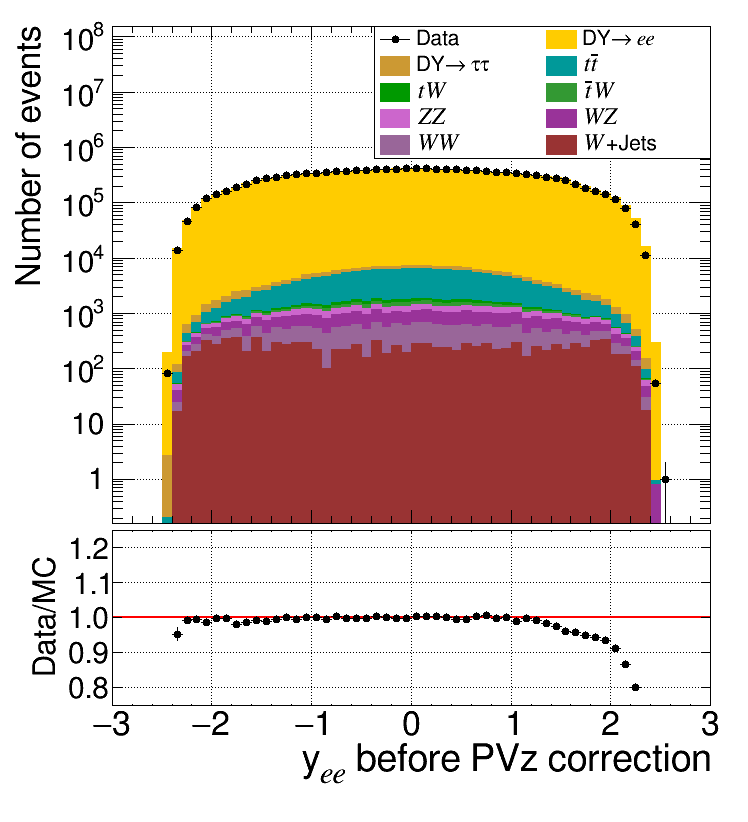
\includegraphics[width=0.48\textwidth]{Magistrinis/ee_rapi_before.png}
	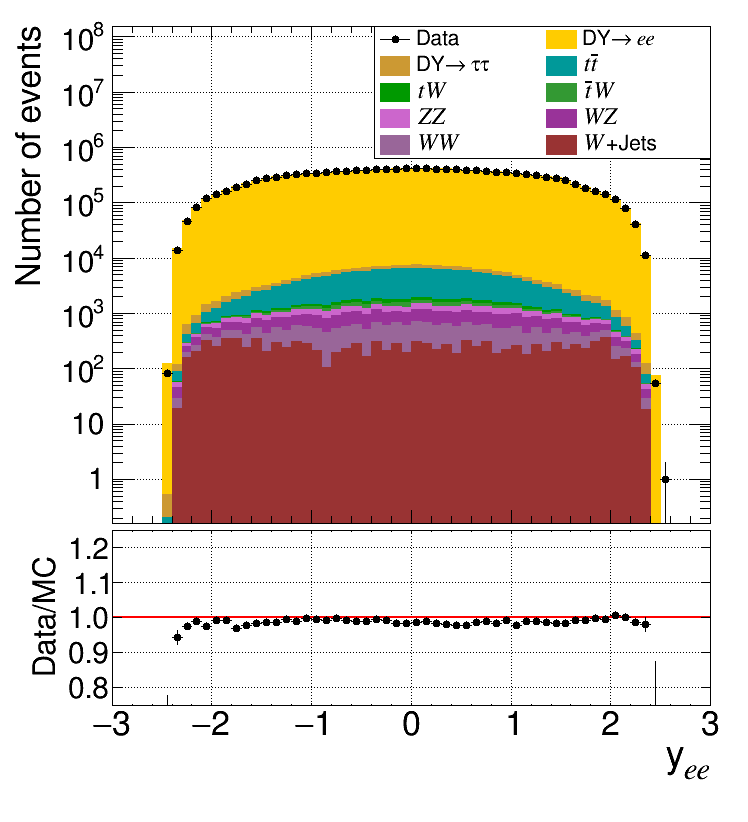
\includegraphics[width=0.48\textwidth]{Magistrinis/ee_rapi_after.png}
	\vspace{-0.5cm}
	\caption{\label{fig:rapiba} Elektronų porų spartos pasiskirstymai prieš ir po pirminės viršūnės $z$ koordinatės bei per ankstaus
	trigerio suveikimo pataisų pritaikymo.}
\end{figure}

Kai kuriuos nesutapimus gali nulemti ir neidealios teorinės žinios apie tam tikrus didelių energijų fizikos procesus.
CMS kolektyvo viršūninio kvarko ir antikvarko porų ($\ttbar\,$) tyrėjai jau anksčiau buvo pastebėję, jog eksperimentiškai
išmatuoti viršūninių kvarkų skersinio impulso pasiskirstymai turi reikšmingų nesutapimų su teoriniais pasiskirstymais,
gautais modeliuojant antros eilės perturbacijų (NLO) tikslumu \cite{ttbarPT}.
Šių tikėtinumų neatitikimai buvo taisomi modeliuotiems $\ttbar\,$ įvykiams priskiriant viršūninio kvarko tyrimo grupės
siūlomus svorinius daugiklius.
Šie daugikliai turėtų priartinti modeliuotą viršūninių kvarkų skersinių impulsų pasiskirstymą prie naujausių eksperimentinių rezultatų.
Jų vertės nustatomos iš kvarkų skersinių impulsų $(p_{t})_{\mathrm{T}}$ verčių.
Tipinės svorinių daugiklių vertės buvo didesnės už vienetą, kai abiems kvarkams $(p_{t})_{\mathrm{T}}<120$~GeV, ir mažesnės už vienetą,
kai abiems kvarkams $(p_{t})_{\mathrm{T}}>120$~GeV.

Visi svoriniai daugikliai iš skirtingų pataisų buvo tarpusavyje sudauginami, gaunant galutinį pataisos daugiklį, skirtą vienam įvykiui.
Kiekvienam modeliuotam įvykiui priskiriamas svoris $\omega_i$ pildant histogramas buvo nustatomas sudauginant normuojantį įvykio daugiklį,
gautą iš \eqref{eq:NLOweight} formulės, su galutiniu pataisos daugikliu:
\begin{equation}
\label{eq:weightCorr}
	\omega_i = \omega_{i}^{\mathrm{Gen.}} \frac{ \sigma\Lumi }{ \sum_{j=1}^{N}\omega_{j}^{\mathrm{Gen.}} }
			   \left[ \prod_{\mathrm{Corr.}} \omega_i^{\mathrm{Corr.}} \right] ,
\end{equation}
čia $\sigma$ -- proceso reakcijos skerspjūvis, $\Lumi$ -- integruotas šviesis, $\omega_{i}^{\mathrm{Gen.}}$ -- modeliavimo
programos įvykiui priskirtas svoris, $\omega_i^{\mathrm{Corr.}}$ -- tam tikros pataisos įvykiui priskirtas svoris.


\subsection{Klaidingo atpažinimo tikimybės matavimas}\label{sec:FRmeasure}
Klaidingo atpažinimo metodas buvo naudojamas įvertinti su viena ($\WJets$) ir dviem ($\QCD$) klaidingai kaip leptonai
atpažintomis čiurkšlėmis susijusių triukšmo įvykių skaičių.
Teorinis klaidingo atpažinimo metodo veikimo principas yra aprašytas \ref{sec:FR} skyriuje.
Eksperimentiškai klaidingo atpažinimo tikimybė buvo matuojama skaičiuojant, kokia dalis atlaisvintus leptonų atrankos
kriterijus praėjusių klaidingai atpažintų čiurkšlių gali praeiti ir Drell-Yan proceso atranką, kurios kriterijai nurodyti
\ref{table:selection} lentelėje.
Kitaip tariant, buvo apibrėžiamos signalo (praeinama griežta atranka) ir kontrolinė sritys (praeinama tik atlaisvinta
atranka, o griežta nepraeinama), o klaidingo atpažinimo tikimybė buvo nustatoma pagal tokią formulę:
\begin{equation}
	\label{eq:FRexp}
	f = \frac{N_{\mathrm{Signal}}^{\QCD}}{N_{\mathrm{Signal}}^{\QCD}+N_{\mathrm{Control}}^{\QCD}},
\end{equation}
čia indeksai \ltq{signal} ir \ltq{control} žymi signalo ir kontrolinę sritis, o indeksas \ltq{$\QCD$} pažymi, kad
skaičiuojamas tik su $\QCD$ procesu susijusių įvykių skaičius.
Taip daroma todėl, kad skaičiuojant klaidingo atpažinimo tikimybę mus domina tik klaidingai atpažinti leptonai,
o $\QCD$ procese tikrų izoliuotų leptonų nėra.
Konkretūs įvykių atrankos kriterijai, naudoti signalo ir kontrolinei sritims apibrėžti elektronų ir miuonų kanaluose,
pateikti \ref{table:FR} lentelėje.

\begin{table}[!b]
	\begin{tabular}{|c|c|c|c|}
		\hline
		\multicolumn{2}{|c|}{\textbf{Miuono objektai}} & \multicolumn{2}{c|}{\textbf{Elektrono objektai}} \\
		\hline
		\textbf{Signalo sritis} & \textbf{Kontrolinė sritis} & \textbf{Signalo sritis} & \textbf{Kontrolinė sritis} \\
		\hline\hline
		\multicolumn{2}{|c|}{\multirow{2}{15em}{\centering Aukšto lygio trigeris \ttt{HLT\_Mu50}}} &
			\multicolumn{2}{c|}{\multirow{2}{20em}{\centering Aukšto lygio trigerių \ttt{HLT\_PhotonX} kombinacija
				(\ttt{X} $=22, 30, 36, 50, 75, 90, 120, 175$)}} \\
		\multicolumn{2}{|c|}{ } & \multicolumn{2}{c|}{ } \\
		\hline
		\multicolumn{2}{|c|}{$\pT>52$~GeV} & \multicolumn{2}{c|}{$\pT>25$~GeV} \\
		\hline
		\multicolumn{2}{|c|}{$|\eta|<2.4$} & \multicolumn{2}{c|}{$|\eta|<2.4$}\\
		\hline
		\multicolumn{2}{|c|}{\multirow{6}{15em}{\centering \ltq{\ttt{TightID}} reikalavimai}} &
			\multicolumn{2}{c|}{Trūkstamų pataikymų skaičius $N_{MH}\leqslant1$} \\ \cline{3-4}
		\multicolumn{2}{|c|}{ } & \multicolumn{2}{c|}{\multirow{3}{20em}{\centering Pataikymams į EM kalorimetro cilindrą:\\ $\sigma_{i\eta i\eta}<0.013$,
				$H/E<0.13$,\\ $|\Delta\eta_{\mathrm{in}}^{\mathrm{seed}}|<0.01$, $|\Delta\phi_{\mathrm{in}}|<0.07$}} \\
		\multicolumn{2}{|c|}{ } & \multicolumn{2}{c|}{ } \\
		\multicolumn{2}{|c|}{ } & \multicolumn{2}{c|}{ } \\ \cline{3-4}
		\multicolumn{2}{|c|}{ } & \multicolumn{2}{c|}{{\multirow{2}{20em}{\centering Pataikymams į EM kalorimetro antgalius:\\
			$\sigma_{i\eta i\eta}<0.035$, $H/E<0.13$}}} \\
		\multicolumn{2}{|c|}{ } & \multicolumn{2}{c|}{ } \\
		\hline
		\multirow{2}{7em}{\centering $I_{\mathrm{PF}}^{\mathrm{rel.}} < 0.15$} &
			\multirow{2}{8em}{\centering $I_{\mathrm{PF}}^{\mathrm{rel.}} > 0.15$} &
			\multirow{2}{8em}{\centering \ltq{\ttt{MediumID}} reikalavimai} &
			\multirow{2}{12em}{\centering Netenkinami \ltq{\ttt{MediumID}} reikalavimai} \\
		 & & & \\
		\hline
	\end{tabular}
	\caption{\label{table:FR} Naudoti miuono ir elektrono objektų atrankos kriterijai signalo ir kontrolinei sritims.
	Elektrono objektams naudoti atrankos kriterijams naudoti dydžiai $\sigma_{i\eta i\eta}$, $H/E$,
	$|\Delta\eta_{\mathrm{in}}^{\mathrm{seed}}|$ ir $|\Delta\phi_{\mathrm{in}}|$ yra paaiškinti CMS elektrono ir fotono fizikinių
	objektų mokslinės grupės straipsnyje \cite{EleID}.}
\end{table}


Atlaisvinta miuonų atranka buvo atliekama naudojant aukšto lygio vieno neizoliuoto miuono trigerį, kuris aktyvuojamas,
kai aptinkamas miuono objektas su skersiniu impulsu, didesniu, nei $50$~GeV.
Iš trigerį aktyvavusių įvykių buvo atrenkami miuonai, kurie atitinka CMS miuonų fizikinių objektų mokslinės grupės nustatytus
labai griežtus miuonų atpažinimo reikalavimus bei savo kampinėmis koordinatėmis sutampa su trigerį aktyvavusiu fizikiniu objektu.
Atsižvelgiant į trigerio ir miuonų detektorių veikimo efektyvumus, buvo reikalaujama, kad miuonų skersinis impulsas viršytų
$52$~GeV, o jų pseudospartos absoliutinė vertė būtų mažesnė už $2.4$.
Signalo ir kontrolinė sritys buvo atskiriamos pagal pagrindinėje miuonų atrankoje (žr.\ \ref{table:selection} lentelę) taikytą
trajektorijos izoliuotumo kriterijų: miuonai, tenkinantys izoliuotumo reikalavimą, patenka į signalo, o jo netenkinantys --
į kontrolinę sritį.
Taip pat, siekiant atmesti Drell-Yan signalą ir kitus su tikrų leptonų poromis susijusius įvykius (matuojant klaidingo
atpažinimo tikimybę mus domina tik \ltq{netikri} leptonai), įvykiai su dviem ir daugiau miuonų, patenkančių į signalo sritį,
buvo atmetami.

Atlaisvinta elektronų atranka buvo atliekama naudojant aštuonių aukšto lygio vieno fotono trigerių su skirtingais skersinio impulso
slenksčiais kombinaciją.
Verta atkreipti dėmesį, kad elektronai taip pat gali aktyvuoti fotono trigerius, nes šie nesiremia CMS trekų detektoriaus informacija.
Šie trigeriai aktyvuojami taip dažnai, kad jiems buvo taikomas tarpavimas: išsaugoma tik tam tikra dalis trigerį turinčių
aktyvuoti įvykių.
Kiekvienam iš naudotų trigerių buvo taikoma skirtinga tarpavimo vertė, o taip pat visos vertės buvo keičiamos realiu laiku duomenų
rinkimo metu, priklausomai nuo eksperimento sąlygų.
Kadangi modeliuotuose duomenyse trigerių tarpavimas nėra taikomas, norint tiesiogiai lyginti eksperimentą su modeliavimu,
tarpavimą reikėjo atitaisyti.
Tai buvo daroma kiekvienam CMS detektoriaus užregistruotam įvykiui pritaikant svorinį daugiklį, lygų nustatytai aktyvuoto
trigerio tarpavimo vertei tuo metu, kai nagrinėjamas įvykis buvo užregistruotas.
Atranką praėjusių elektrono objektų skersinių impulsų pasiskirstymai prieš ir po trigerių tarpavimo atitaisymo, palyginti
\ref{fig:prescale} pav.

\begin{figure}[t!]
	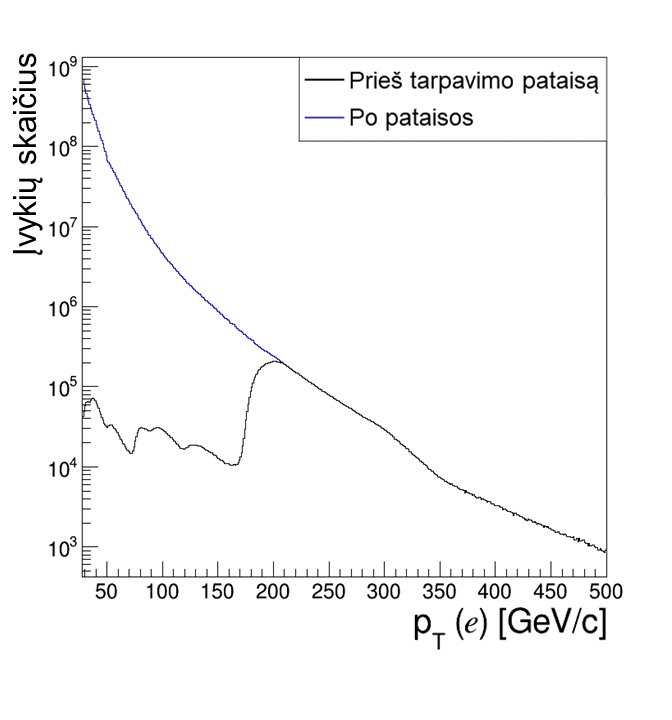
\includegraphics[width=0.5\textwidth]{Magistrinis/prescale.png}
	\vspace{-1.2cm}
	\caption{\label{fig:prescale} Elektrono objektų skersinio impulso pasiskirstymai prieš ir po trigerių tarpavimo
	atitaisymo (žr.\ legendą).}
\end{figure}

Trigerį aktyvavusiems elektrono objektams buvo taikomi papildomi atrankos reikalavimai, atitinkantys pagrindinėje įvykių
atrankoje (žr.\ \ref{table:selection} lentelę) naudojamo dviejų elektronų trigerio taikomus reikalavimus fizikiniams objektams.
Tai -- reikalavimai elektrono objekto palikto signalo formai elektromagnetiniame kalorimetre bei reikalavimai
trekų detektoriaus ir kalorimetro užregistruotos informacijos sutapimui.
Taip pat buvo taikomas kriterijus, reikalaujantis ne daugiau kaip vieno trūkstamo pataikymo trekų detektoriuje toje vietoje, per
kurią eina elektrono objekto trajektorija (trūkstami pataikymai gali byloti apie elektrono atsiradimą antrinių procesų metu).
Atsižvelgiant į naudojamų trigerių ir CMS detektoriaus komponentų efektyvumus, buvo reikalaujama, kad elektronų skersinis
impulsas viršytų $25$~GeV, o pseudosparta neviršytų $|\eta|<2.4$.
Atlaisvintą atranką praėję elektronai į signalo ir kontrolinę sritis buvo skirstomi pagal tai, ar jie tenkina CMS elektrono
ir fotono fizikinių objektų mokslinės grupės nustatytus vidutiniškai griežtus elektrono atpažinimo reikalavimus, ar ne.
Analogiškai, kaip ir su miuonais, elektronų įvykiai taip pat buvo atmetami, jeigu juose yra daugiau negu vienas į signalo
sritį patenkantis elektrono objektas.
Vis dėlto, čia buvo papildomai stengiamasi atmesti ir su $\WJets$ procesu susijusius tikrus elektronus, todėl buvo taikomas
reikalavimas, kad skersinio impulso trūkumas įvykyje neviršytų $25$~GeV ($W$ bozono skilimo metu susidaręs neutrinas tipiškai
turi didelį skersinį impulsą).

Klaidingo atpažinimo tikimybės matavimui pagal \eqref{eq:FRexp} formulę reikėjo išskirti signalo ir kontrolinėje srityje esančius
su $\QCD$ procesu susijusius klaidingai atpažintus leptonus.
$\QCD$ įvykių skaičius buvo įvertinamas kombinuojant matavimą ir modeliavimą skirtingais būdais.
Miuonams buvo taikomi du metodai:
\begin{enumerate}
	\item Santykio metodas: $\QCD$ įvykių skaičius gaunamas padauginus išmatuotą įvykių skaičių iš sumodeliuoto $\QCD$ ir visų
	galimų procesų santykio:
	\begin{equation}
		N_i^{\QCD}=N_i^{\mathrm{Data}} \frac{N_i^{\QCD \, \mathrm{MC}}}{N_i^{\mathrm{All \, MC}}},
	\end{equation}
	čia ir toliau $i$ gali būti \ltq{Signal} arba \ltq{Control}.
	\item Šablonų priderinimo (angl.\ \textit{template fitting}) metodas: $\QCD$ įvykių skaičius gaunamas pasirinkus vieną
	įvykius apibūdinantį parametrą ir mažiausių kvadratų metodu priderinus šio parametro pasiskirstymus skirtingiems procesams
	(šablonus) prie eksperimento metu išmatuoto pasiskirstymo.
	Šiuo atveju buvo naudojamas dalelių srauto algoritmo apskaičiuojamas trajektorijos izoliuotumo parametras.
	Skirtingų procesų šablonus galima gauti įvairiais būdais, bet šiuo atveju šablonai buvo gauti pasinaudojant modeliavimu:
	\begin{equation}
		N_i^{\mathrm{Data}} \approx \alpha_i^{\QCD} N_i^{\QCD \, \mathrm{MC}} + \alpha_i^{\WJets} N_i^{\WJets \, \mathrm{MC}} +
		\alpha_i^{\mathrm{DY}} N_i^{\mathrm{DY \, MC}} + \dots \;,
	\end{equation}		
	čia $\alpha$ su atitinkamais indeksais -- pataisos parametrai, kurių vertės nustatomos priderinimo metu.
	Nustačius parametrų $\alpha$ vertes, į \eqref{eq:FRexp} išraišką statomas $\QCD$ įvykių skaičius įvertinamas kaip
	$N_i^{\QCD} = \alpha_i^{\QCD} N_i^{\QCD \, \mathrm{MC}}$.
\end{enumerate}

Elektronams kokybiškai sumodeliuotas $\QCD$ duomenų rinkinys nebuvo prieinamas, todėl jiems $\QCD$ įvykių skaičius buvo
įvertinamas atimties metodu -- iš eksperimento metu išmatuoto įvykių skaičiaus atimant sumodeliuotą visų su $\QCD$ procesu
nesusijusių įvykių skaičių:
\begin{equation}
	N_i^{\QCD} = N_i^{\mathrm{Data}} - N_i^{\mathrm{non}{\text -}\QCD \, \mathrm{MC}}.
\end{equation}
Klaidingo atpažinimo tikimybės matavimui skirtiems modeliuotiems įvykiams buvo pritaikytos visos \ref{sec:corrections}
skyriuje aprašytos pataisos, išskyrus efektyvumų pataisas, nes šios buvo tinkamos  naudoti tik su tikrais izoliuotais leptonais.
Klaidingo atpažinimo tikimybė buvo matuojama kaip funkcija nuo fizikinio objekto skersinio impulso ir pseudospartos,
t.y., buvo sudalinta į tam tikro pločio skersinio impulso ir pseudospartos sritis.
Klaidingo atpažinimo tikimybė nuo pseudospartos priklauso nežymiai: rimtesni kiekybiniai skirtumai pastebimi tik
tarp tikimybių būti klaidingai atpažintiems objektams, pataikiusiems į detektoriaus cilindrinę ir antgalių dalis.
Todėl pagal pseudospartą klaidingo atpažinimo tikimybės buvo dalinamos tik į dvi dalis, atitinkančias detektoriaus cilindrą
ir antgalius.

\subsection{Su čiurkšlėmis susijusių triukšmo įvykių skaičiaus įvertinimas} \label{sec:bkgEst}
Klaidingo atpažinimo tikimybę galima panaudoti įvertinant, kiek su klaidingai atpažintomis čiurkšlėmis susijusių
triukšmo įvykių pateko į Drell-Yan signalo atrankos kriterijus tenkinančių įvykių rinkinį $N_{\mathrm{SS}}$
(žr.\ \eqref{eq:2passFR} formulę).
Drell-Yan proceso atranką praeina įvykiai su dviem izoliuotais leptono objektais (žr.\ \ref{table:selection} lentelę),
tad galimas dvejopas su klaidingai atpažintomis čiurkšlėmis susijęs triukšmas: klaidingai atpažinta kaip \ltq{geras}
leptonas gali būti viena ($\WJets$) arba dvi ($\QCD$) čiurkšlės.
Žinant klaidingo atpažinimo tikimybę, su tokiais triukšmais susijusių įvykių skaičių galima įvertinti pasinaudojant įvykių
rinkiniais, kuriuose viena arba dvi leptonus imituojančios čiurkšlės praėjo tik atlaisvintą leptono objektų atranką, bet netenkino
griežtesnių pagrindinėje analizėje naudojamų reikalavimų: $N_{\mathrm{SC+CS}}$ ir $N_{\mathrm{CC}}$.
Šie duomenų rinkiniai buvo gaunami kombinuojant pagrindinės analizės ir klaidingo atpažinimo tikimybės matavimui skirtus
įvykių atrankos kriterijus.
Naudoti atrankos kriterijai apibendrinti \ref{table:jetSelection} lentelėje.

\begin{table}[!t]
	\begin{tabular}{|c|c|c|c|}
		\hline
		\multicolumn{2}{|c|}{\textbf{\textit{µµ} įvykiai}} & \multicolumn{2}{c|}{\textbf{\textit{ee} įvykiai}} \\
		\hline
		\textbf{$\WJets$ atranka} & \textbf{$\QCD$ atranka} & \textbf{$\WJets$ atranka} & \textbf{$\QCD$ atranka} \\
		\hline\hline
		\multicolumn{2}{|c|}{Aukšto lygio trigeris: jokio} & \multicolumn{2}{c|}{Aukšto lygio trigeris: \ttt{HLT\_Ele23Ele12}} \\
		\hline
		\multicolumn{4}{|c|}{$(p_1)_\mathrm{T} > 28$~GeV, $(p_2)_\mathrm{T} > 17$~GeV} \\
		\hline
		\multicolumn{2}{|c|}{$|\eta| < 2.4$} &
			\multicolumn{2}{c|}{$|\eta_{\mathrm{SC}}| < 2.4$, išskyrus $1.4442 < |\eta_{\mathrm{SC}}| < 1.566$} \\
		\hline
		\multicolumn{2}{|c|}{\ltq{\ttt{TightID}} reikalavimai} &
			\multicolumn{2}{c|}{Trūkstamų pataikymų skaičius $N_{MH}\leqslant1$} \\
		\hline
		\multicolumn{2}{|c|}{\multirow{3}{16em}{\centering Pasirenkami 2 miuonai, kuriuos galima tiksliausiai suvesti į vieną
			pirminę viršūnę su $\chi^2<20$}} &
			\multicolumn{2}{c|}{\multirow{3}{19em}{\centering Pataikymams į EM kalorimetro cilindrą:\\ $\sigma_{i\eta i\eta}<0.013$,
				$H/E<0.13$,\\ $|\Delta\eta_{\mathrm{in}}^{\mathrm{seed}}|<0.01$, $|\Delta\phi_{\mathrm{in}}|<0.07$}} \\
		\multicolumn{2}{|c|}{ } & \multicolumn{2}{c|}{ } \\
		\multicolumn{2}{|c|}{ } & \multicolumn{2}{c|}{ } \\
		\hline
		\multicolumn{2}{|c|}{\multirow{2}{16em}{\centering Priešingi elektriniai krūviai}} &
			\multicolumn{2}{c|}{\multirow{2}{19em}{\centering Pataikymams į EM kalorimetro antgalius:\\
				$\sigma_{i\eta i\eta}<0.035$, $H/E<0.13$}} \\
		\multicolumn{2}{|c|}{ } & \multicolumn{2}{c|}{ } \\
		\hline
		\multicolumn{2}{|c|}{\multirow{2}{16em}{\centering Plokštuminis kampas\\ $\alpha < \pi - 0.005$ rad}} & 
			\multicolumn{2}{c|}{\multirow{2}{19em}{\centering Atrankos reikalavimus turi atitikti lygiai 2 elektronai}} \\
		\multicolumn{2}{|c|}{ } & \multicolumn{2}{c|}{ } \\
		\hline
		\multirow{3}{9em}{\centering Vienam miuonui $I_{\mathrm{PF}}^{\mathrm{rel.}}<0.15$,
			kitam -- $I_{\mathrm{PF}}^{\mathrm{rel.}}\geqslant 0.15$} &
			\multirow{3}{7em}{\centering Abiems miuonams $I_{\mathrm{PF}}^{\mathrm{rel.}}\geqslant 0.15$} &
			\multirow{3}{10em}{\centering Vienas elektronas tenkina \ltq{\ttt{MediumID}} reikalavimus, kitas -- ne} &
			\multirow{3}{10em}{\centering Abu elektronai netenkina \ltq{\ttt{MediumID}} reikalavimų} \\
		 & & & \\
		 & & & \\
		\hline
	\end{tabular}
	\caption{\label{table:jetSelection} Apibendrinti atrankos kriterijai įvykių rinkiniams, naudotiems vienos ($\WJets$) ir
	dviejų ($\QCD$) klaidingai atpažintų čiurkšlių triukšmams įvertinti $ee$ ir $\mu\mu$ kanaluose.
	$(p_1)_\mathrm{T}$ ir $(p_2)_\mathrm{T}$ žymi atitinkamai greitesniojo ir lėtesniojo leptono skersinį impulsą.
	Elektrono objektams naudoti dydžiai $\sigma_{i\eta i\eta}$, $H/E$,
	$|\Delta\eta_{\mathrm{in}}^{\mathrm{seed}}|$ ir $|\Delta\phi_{\mathrm{in}}|$ yra paaiškinti CMS elektrono ir fotono
	fizikinių objektų mokslinės grupės straipsnyje \cite{EleID}.}
\end{table}


\begin{figure}[b!]
	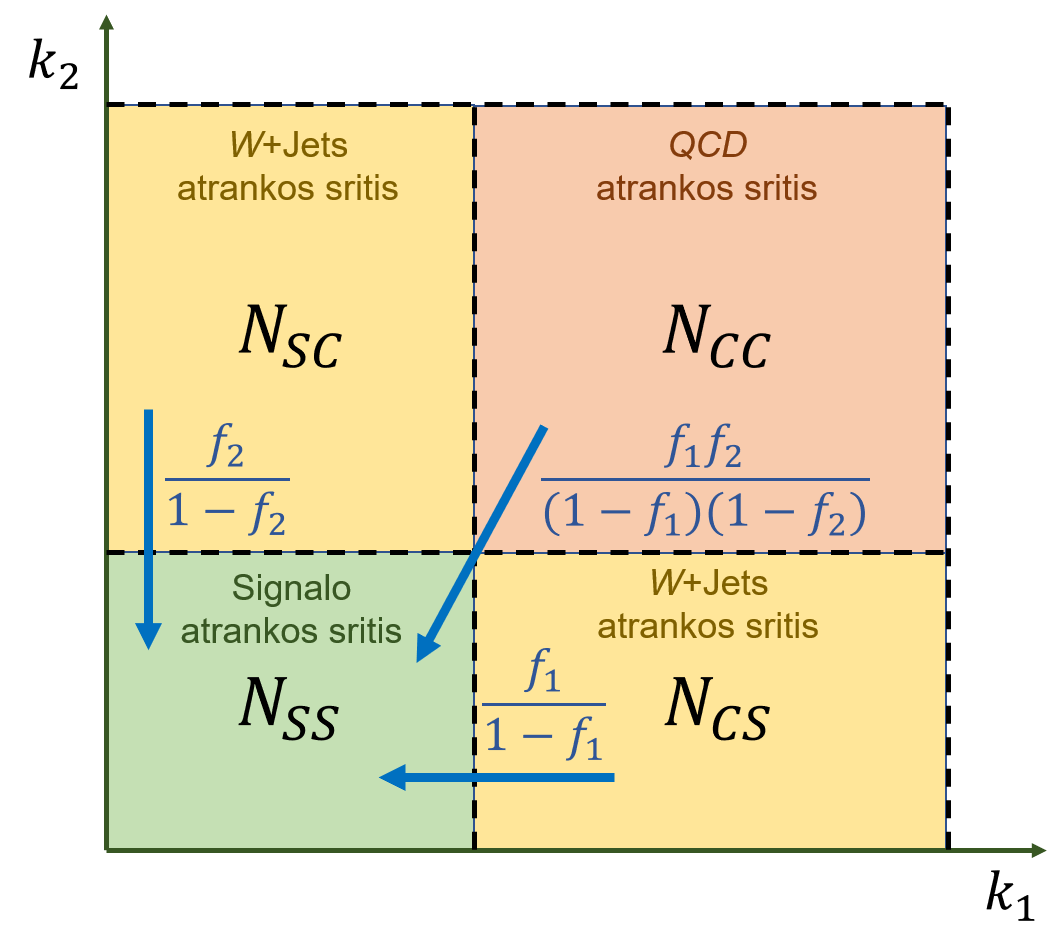
\includegraphics[width=0.5\textwidth]{Magistrinis/FRschema.png}
	\vspace{-0.3cm}
	\caption{\label{fig:FRscheme}Klaidingo atpažinimo metodo taikymo schema.
	Ant ašių esantys dydžiai $k_1$ ir $k_2$ vaizduoja pirmam ir antram elektrono objektui taikomų atrankos
	kriterijų laisvumą.}
\end{figure}


Triukšmo įvykių skaičiaus įvertinimo schema, iliustruojanti triukšmo įverčių perkėlimą iš $\WJets$ ir $\QCD$ atrankos sričių
į signalo atrankos sritį, pavaizduota \ref{fig:FRscheme} pav.
Schemoje žalia spalva vaizduojama griežčiausiais kriterijais apribota Drell-Yan signalo atrankos sritis.
Į geltonai pažymėtas $\WJets$ atrankos sritis patenka įvykiai, kuriuose vienas objektas iš dviejų praėjo tik atlaisvintą atranką,
bet nepraėjo griežtos atrankos, o į raudonai pažyėtą $\QCD$ atrankos sritį -- įvykiai, kuriuose du objektai nepraėjo griežtos atrankos.
Išraiškos prie mėlynų rodyklių vaizduoja svorinius daugiklius, naudojamus perkelti triukšmo įvykių įverčius iš $\WJets$
ir $\QCD$ atrankos sričių į Drell-Yan signalo atrankos sritį.

Įvykių su dviem klaidingai atpažintomis čiurkšlėmis skaičius buvo įvertinamas pasinaudojant įvykiais, kuriuose abu užfiksuoti
leptono objektai praėjo atlaisvintus atrankos kriterijus, bet netenkino griežtesnių pagrindinės analizės reikalavimų (t.y., abu
miuonai nepraėjo trajektorijos izoliuotumo reikalavimo arba abu elektronai nepraėjo vidutiniškai griežtų atpažinimo reikalavimų).
Pagal \eqref{eq:2passFR} formulę, kiekvienam tokiam įvykiui buvo priskiriamas svorinis daugiklis $\frac{f_1 f_2}{(1-f_1)(1-f_2)}$.
Kaip galima matyti iš \eqref{eq:2fail} formulės, įvykių rinkinys su dviem leptono objektais $\QCD$ atrankos srityje $N_{\mathrm{CC}}$
yra užterštas įvykiais, turinčiais tikrų leptonų, kurie dėl įvairių priežasčių nepraėjo griežtesnių atrankos reikalavimų.
Su tikrais leptonais susiję įvykiai buvo atmesti pasinaudojant modeliavimu.

Įvykių su viena klaidingai atpažinta čiurkšle skaičius buvo įvertinamas pasinaudojant įvykiais, kuriuose abu leptono objektai
praėjo atlaisvintus atrankos kriterijus, tačiau tik vienas iš jų tenkino ir griežtesnius pagrindinės analizės reikalavimus.
Pagal \eqref{eq:2passFR} formulę, kiekvienam tokiam įvykiui buvo priskiriamas svorinis daugiklis $f/(1-f)$.
Panašiai, kaip ir $\QCD$ atrankos atveju, šis duomenų rinkinys yra užterštas įvykiais, kuriuose susidarė du tikri leptonai,
iš kurių vienas netenkino griežtesniųjų reikalavimų bei įvykiais, kuriuose viena iš dviejų leptonus imituojančių čiurkšlių tenkina
ne tik atlaisvintus, bet ir griežtesniuosius reikalavimus (žr.\ \ref{eq:realfake} formulę).
Dviejų tikrų leptonų įvykiai buvo atmesti pasinaudojant modeliavimu, o dviejų čiurkšlių įvykiai -- pasinaudojant įverčiu, gautu
iš $\QCD$ atrankos srities (tik šį įvertį reikėjo padauginti iš dviejų, kad būtų įvertinta galimybė bet kuriai iš dviejų
klaidingai atpažintų čiurkšlių atitikti griežtesniuosius reikalavimus).

Analogiškai buvo galima įvertinti su klaidingai atpažintomis čiurkšlėmis susijusių triukšmo įvykių skaičių ne tik elektronų
ir miuonų kanaluose, bet ir įvykių rinkinyje su priešingo krūvio elektrono-miuono pora.
Toks duomenų rinkinys yra naudojamas taikant matavimu grįstą $\emu$ metodą, kuris skirtas įvertinti su tikrais leptonais susijusių
Drell-Yan proceso triukšmo įvykių skaičių \cite{MAbak}.
Šio metodo įvertį galima patikslinti iš naudojamo duomenų rinkinio atmetus su klaidingai atpažintomis čiurkšlėmis susijusius
įvykius.
Tai buvo padaryta pasinaudojant įvykių rinkiniais, kuriuose elektronas ir/arba miuonas praeina atlaisvintą atranką, bet netenkina
griežtesnių pagrindinės įvykių atrankos reikalavimų.
Triukšmo įvykių skaičius buvo įvertintas atitinkamiems objektams naudojant išmatuotas elektrono arba miuono klaidingo atpažinimo
tikimybes.


\subsection{Matavimo paklaidų įvertinimas}\label{sec:uncertainties}
Eksperimentinėje didelių energijų fizikoje yra laikoma, jog įvykių skaičiaus pasiskirstymus aprašo Puasono dėsnis.
Galima parodyti, kad taip pasiskirsčiusių atsitiktinių įvykių skaičiaus standartinis nuokrypis yra lygus kvadratinei
šakniai iš tikėtiniausio įvykių skaičiaus.
Realybėje tikėtiniausias įvykių skaičius nėra žinomas dydis, todėl tenka padaryti prielaidą, kad eksperimento metu išmatuotas
įvykių skaičius yra artimas labiausiai tikėtinam.
Tokiu atveju statistiniu užregistruotų įvykių skaičiaus neapibrėžtumu laikome kvadratinę šaknį iš jo paties.

Dėl normavimo ir taikytų pataisų, modeliuoti įvykiai turėjo nelygius vienetui svorius $\omega_i$, apskaičiuojamus pagal
\eqref{eq:weightCorr} formulę.
Statistine įvykių su nevienetiniais svoriais skaičiaus neapibrėžtimi buvo laikoma kvadratinė šaknis iš visų įvykių svorių
kvadratų sumos:
\begin{equation}
	(\Delta N)_{\mathrm{Stat.\,}} = \sqrt{\sum_{i=1}^{N}\omega_{i}^{2}} \; .
	\label{eq:Sumw2Unc}
\end{equation}
Matome, kad visų įvykių svorius pakeitus į vienetus grįžtame prie neapibrėžtumo, lygaus kvadratinei šakniai iš įvykių
skaičiaus.

Atkreiptinas dėmesys, kad, turint daugiau faktiškai sumodeliuotų įvykių (čia kalbame apie pačius įvykius, o ne jų svorius)
nei buvo užregistruota eksperimento metu, jiems bus priskiriami mažesni už vienetą svoriai.
Iš \eqref{eq:Sumw2Unc} formulės seka, kad tokiu atveju sunormuoto įvykių skaičiaus statistinė neapibrėžtis bus mažesnė nei
detektoriaus užregistruotų įvykių skaičiaus.
Tai yra vienas iš modeliavimo privalumų, kai modeliuojami mažo tikėtinumo įvykiai.
Tuo tarpu, jeigu modeliuojami labai didelio tikėtinumo įvykiai, priklausomai nuo sumodeliuoto įvykių skaičiaus
jiems gali būti priskiriami smarkiai didesni už vienetą svoriai.
Tokiu atveju statistinė neapibrėžtis gerokai viršys eksperimento metu užregistruotų įvykių neapibrėžtį.
Tai yra viena iš pagrindinių priežasčių, kodėl $\QCD$ ir $\WJets$ triukšmo įvykių skaičiui įvertinimui reikia naudoti
klaidingo atpažinimo (ar kitą) metodą -- šių procesų reakcijos skerspjūviai yra labai dideli (žr.\ \ref{table:Xsec} lentelę),
o tai nulemia didelius statistinius neapibrėžtumus.

Klaidingo atpažinimo metodu įvertinto triukšmo įvykių skaičiaus statistinis neapibrėžtumas buvo skaičiuojamas ne pagal
\eqref{eq:Sumw2Unc} formulę, o ištraukiant kvadratinę šaknį iš gauto rezultato.
Taip buvo padaryta todėl, kad klaidingo atpažinimo tikimybė buvo naudojama kaip svorinis daugiklis kiekvienam įvykiui.
Bendru atveju šio daugiklio vertės buvo labai mažos, todėl neapibrėžtumas, įvertintas naudojantis \eqref{eq:Sumw2Unc}
formule, būtų buvęs netikroviškai mažas.

Sisteminių neapibrėžtumų įvertinimui CMS statistikos komitetas rekomenduoja tą patį dydį įvertinti dviem skirtingais metodais,
kurie idealiu atveju turėtų duoti vienodą rezultatą.
Jeigu matavimai yra nepriklausomi ir lygiaverčiai, galima tikėtis, kad ieškoma tikroji vertė (kuri yra nežinoma) yra kažkur
tarp dviejų gautųjų matavimo rezultatų arba artimoje aplinkoje.
Taigi, vieno metodo įvertį pasirinkus centrine verte, jam galima priskirti sisteminę neapibrėžtį, lygią skirtumui tarp
dviejų skirtingų matavimų.

Viena iš sisteminės neapibrėžties dedamųjų kaip miuonai klaidingai atpažintų čiurkšlių įvertinimui buvo laikomas skirtumas
tarp rezultatų, gautų naudojant dvi skirtingas klaidingo atpažinimo tikimybės įvertinimo metodikas: santykio ir šablonų
priderinimo metodą (šablonų priderinimo metodu gautas įvertis buvo laikomas centrine verte):
\begin{equation}
\label{eq:systUncFRmumu}
	(\Delta N_{\mu\mu}^{\mathcal{P} \; \mathrm{FR}})_{\mathrm{Sist.\,}} =
	\left| N_{\mu\mu}^{\mathcal{P} \; \mathrm{FR}}(\mathrm{Fit}) -
	N_{\mu\mu}^{\mathcal{P} \; \mathrm{FR}}(\mathrm{Ratio}) \right| \;  ;
	\;\;\;\;\; \mathcal{P} = \QCD, \; \WJets \; ,
\end{equation}
čia \ltq{FR}\ žymi klaidingo atpažinimo metodu įvertintą įvykių skaičių, \ltq{Fit} žymi klaidingo atpažinimo tikimybei
įvertinti naudotą šablonų priderinimo metodą, o \ltq{Ratio}\ -- santykio metodą.

Tikimybė čiurkšlei būti klaidingai atpažintai kaip elektronui buvo matuojama tik vienu (atimties) metodu, todėl šiuo
atveju sisteminė paklaida buvo įvertinta paėmus antrą įvertį, gautą šiek tiek modifikavus kontrolinės srities apibrėžimą
(fizikiniams objektams leidžiant pažeisti tik vieną kriterijų iš vidutiniškai griežtų atpažinimo reikalavimų rinkinio):
\begin{equation}
\label{eq:systUncFRee}
	(\Delta N_{ee}^{\mathcal{P} \; \mathrm{FR}})_{\mathrm{Sist.\,}} =
	\left| N_{ee}^{\mathcal{P} \; \mathrm{FR}}(\mathrm{Orig.}) -
	N_{ee}^{\mathcal{P} \; \mathrm{FR}}(\mathrm{Alt.}) \right| \;  ;
	\;\;\;\;\; \mathcal{P} = \QCD, \; \WJets \; ,
\end{equation}
čia \ltq{Orig.} žymi įvertį, gautą naudojant \ref{table:FR} lentelėje nurodytus signalo ir kontrolinės srities apibrėžimus, 
o \ltq{Alt.} -- įvertį, gautą naudojant kitą apibrėžimą kontrolinei sričiai.

Klaidingo atpažinimo tikimybei įvertinti buvo naudojamas baigtinis įvykių skaičius, todėl ji turi savo statistinį neapibrėžtumą.
Šis neapibrėžtumas niekaip neatsispindi galutinio triukšmo įvykių skaičiaus įverčio statistiniame neapibrėžtume, todėl
jis buvo įskaitomas laikant jį papildomu indėliu į sisteminę įverčio paklaidą.
Tai pat į sisteminę paklaidą buvo įskaitoma šablonų priderinimo paklaida, grąžinta priderinimo algoritmo.
Padarius prielaidą, kad skirtingos sisteminio neapibrėžtumo dedamosios yra tarpusavyje nepriklausomos, į pilnąją paklaidą jos
buvo sudedamos pagal Pitagoro teoremą.


\newpage
\section{Rezultatai ir jų aptarimas}
\ref{table:selection} lentelėje išvardintus atrankos kriterijus praėjusių leptonų porų invariantinės masės histogramos
prieš klaidingo atpažinimo metodo pritaikymą pateikiamas \ref{fig:MassBefore}~pav.
Šiose histogramose spalvotais stulpeliais pavaizduoti modeliuoti arba $\emu$ metodu įvertinti (kur įmanoma) įvykių skaičiai.
Verta atkreipti dėmesį, kad modeliuoti $\WJets$ ir $\QCD$ procesų įverčiai turi netolydžius invariantinės masės pasiskirstymus:
įvykių skaičiaus skirtumai tarp gretimų histogramos stulpelių vietomis skiriasi dešimtimis kartų, daug stulpelių yra tušti
net žemų masių srityse (ypač $\QCD$ atveju).
Tai rodo prastą šių dviejų procesų modeliavimo kokybę.
$\QCD$ ir $\WJets$, lyginant su kitais Drell-Yan triukšmo procesais turi labai didelį reakcijos skerspjūvį, tačiau artimą
nuliui tikimybę praeiti Drell-Yan proceso atranką.
Sumodeliavus tiek su šiais procesais susijusių įvykių, kiek leidžia turimi skaičiavimo resursai ($5.8\!\times\!10^8$ $\QCD$ ir
$6.3\!\times\!10^8$ $\WJets$ įvykių), iš jų Drell-Yan proceso miuonų kanalo atranką praeina vos $40$ $\QCD$ ir $1288$ $\WJets$,
o elektronų kanalo -- $36$ $\QCD$ ir $4974$ $\WJets$ įvykiai.
Dėl didelio reakcijos skerspjūvio šiems įvykiams priskiriami dideli svoriai, kurių vertės siekia net iki kelių tūkstančių:
sunormavus įvykius pagal integruotą šviesį buvo gauta $1673\pm1498$ $\QCD$ ir $2704\pm200$ $\WJets$ įvykių, patenkančių į
$\mu\mu$ kanalą ir $3177\pm1897$ $\QCD$ bei $11176\pm378$ $\WJets$ įvykių, patenkančių į $ee$ kanalą. 
Didžiuliai statistiniai neapibrėžtumai paaiškina, kodėl pasiskirstymuose matomi tokie smarkūs netolydumai.
Tai yra pagrindinė priežastis, kodėl šių triukšmų indėlį reikėjo įvertinti matavimu grįstais metodais.

\begin{figure}[b!]
	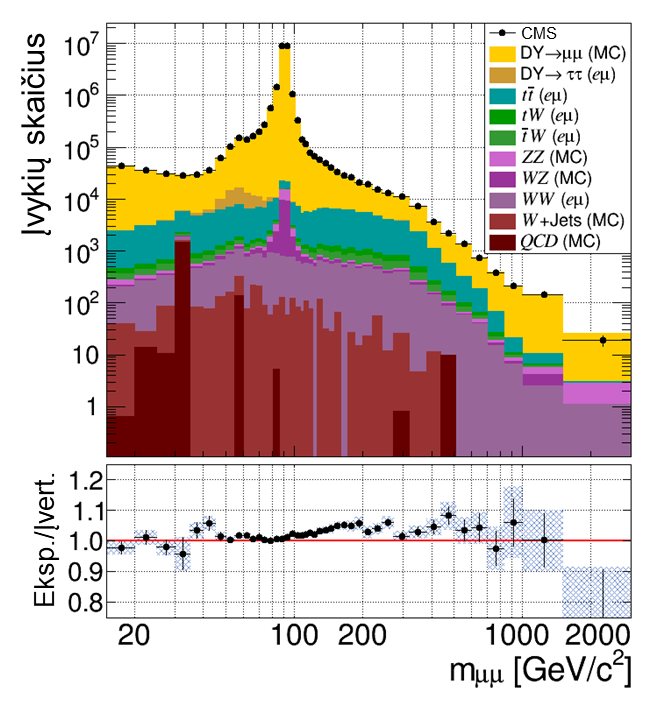
\includegraphics[width=0.49\textwidth]{Magistrinis/MuMumass_beforeFR.png}
	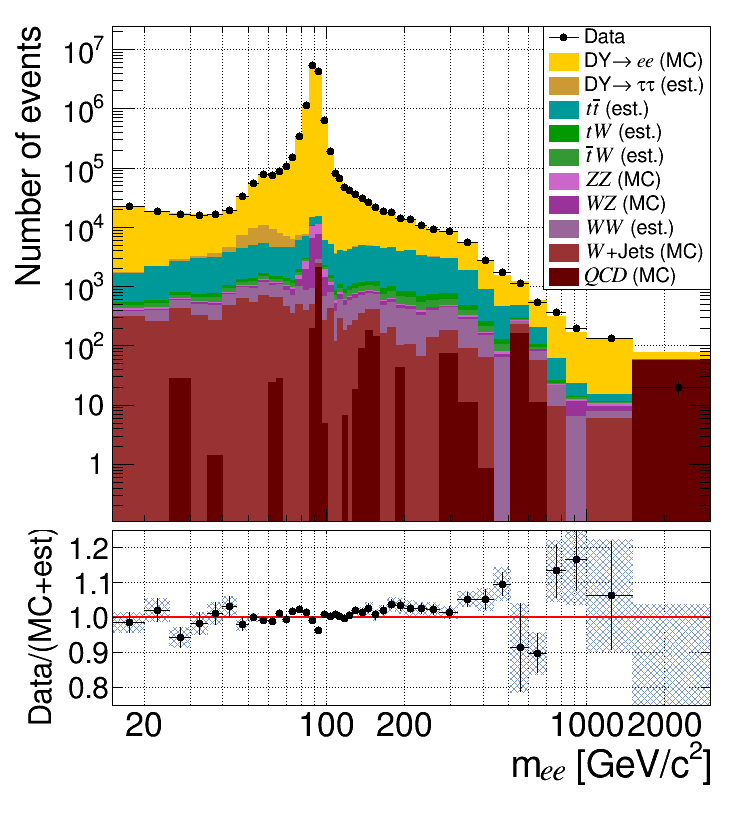
\includegraphics[width=0.49\textwidth]{Magistrinis/EEmass_beforeFR.png}
	\vspace{-0.5cm}
	\caption{\label{fig:MassBefore}
		Miuonų (kairėje) ir elektronų (dešinėje) porų invariantinių masių pasiskirstymai prieš klaidingo atpažinimo metodo
		pritaikymą.
		Juodi taškai vaizduoja CMS detektoriumi išmatuotus pasiskirstymus, o spalvoti stulpeliai -- modeliuotus (legendoje
		žymima \ltq{MC}) arba $\emu$ metodu įvertintus (legendoje žymima \ltq{$\emu$}) įvykius.
		Eksperimento ir įverčio santykio grafike esančios mėlynos juostos vaizduoja suminius (statistinius ir sisteminius)
		neapibrėžtumus.}
\end{figure}

Įvykiai klaidingo atpažinimo tikimybei įvertinti buvo atrenkami pagal \ref{table:FR}~lentelėje nurodytus atrankos kriterijus.
Atranką praėjusių miuono objektų skersinių impulsų pasiskirstymai pateikti \ref{fig:FRpT_mu} pav.
Su $\QCD$ procesu susijusių įvykių skaičiui (jie naudojami klaidingo atpažinimo tikimybei matuoti) detektoriaus išmatuotuose
duomenyse įvertinti buvo pasitelkiami modeliuoti įvykių rinkiniai (žr.\ \ref{sec:FRmeasure} skyrių).
Miuono objektams nesutapimas tarp išmatuoto ir modeliuoto skersinio impulso pasiskirstymo srityje iki $500$~GeV siekė $10-15\%$.
Dėl tokio didelio skirtumo buvo laikoma, kad klaidingo atpažinimo tikimybės matavimas santykio metodu gali būti nepakankamai tikslus.
Tikslesniam klaidingo atpažinimo tikimybės matavimui buvo pasitelktas šablonų priderinimo metodas.
Prie eksperimento priderinus miuono trajektorijos izoliuotumo parametro pasiskirstymus (priderinti pasiskirstymai pateikiami 3 priede)
buvo gauti pataisos daugikliai modeliuotiems duomenų rinkiniams.
$\QCD$ procesui pataisos daugiklis siekė vidutiniškai $0.75$ detektoriaus cilindrinėje ir $0.65$ antgalių dalyje.
Šablonų priderinimo metodu pataisyti miuono objektų skersinio impulso pasiskirstymai pavaizduoti \ref{fig:FRpT_muTFIT} pav.
Pritaikius šablonų priderinimą nesutapimas tarp eksperimentinių ir modeliuotų pasiskirstymų srityje iki $500$~GeV neviršija $10\%$
(išskyrus vieną stulpelį), todėl centrine klaidingo atpažinimo tikimybės verte buvo laikoma gautoji šablonų priderinimo metodu.

Klaidingo atpažinimo tikimybei įvertinti naudota įvykių atranką praėjusių elektrono objektų skersinių impulsų pasiskirstymai
pavaizduoti \ref{fig:FRpT_e} pav.
Elektronų atveju modeliuotas $\QCD$ duomenų rinkinys nebuvo prieinamas (turėtas elektromagnetiniais objektais praturtintas
$\QCD$ duomenų rinkinys davė dvigubai mažesnį rezultatą nei eksperimentas, o brėžti testiniai pasiskirstymai, lyginant su
eksperimentu turėjo kokybinių skirtumų, todėl šio rinkinio naudojimo buvo atsisakyta įtariant, kad jame įskaitomos ne visos
galimybės čiurkšlei imituoti elektroną).
Dėl šios priežasties klaidingo atpažinimo tikimybei įvertinti buvo naudojamas atimties metodas (žr.\ \ref{sec:FRmeasure} skyrių).
Visas \ref{fig:FRpT_e} pav.\ matomas skirtumas tarp eksperimentinių ir modeliuotų pasiskirstymų buvo priskirtas $\QCD$ procesui.

Buvo nustatyta, jog į signalo sritį patenka $2.91\!\times\!10^6$ miuonus ir $1.38\!\times\!10^8$ elektronus imituojančių čiurkšlių,
o į kontrolinę sritį -- $2.87\!\times\!10^7$ miuonus ir $2.87\times10^9$ elektronus imituojančių čiurkšlių.
Tai duoda vidutines klaidingo atpažinimo tikimybes $\bar{f}_{\mu}=9.21\%$ ir $\bar{f}_{e}=4.59\%$ (kur $\bar{f}_{\mu}$ -- tikimybė
miuoną imituojančiai čiurkšlei patekti į signalo sritį, o $\bar{f}_{e}$ -- elektroną imituojančiai čiurkšlei patekti į signalo sritį.
Tikimybė $\bar{f}_{\mu}$ yra didesnė už $\bar{f}_{e}$ dėl pasirinktų sričių apibrėžimų.
$\bar{f}_{\mu}$ vertė pažymi, kad tarp
miuonus imituojančių čiurkšlių, kurios tenkina atlaisvintus miuono atrankos kriterijus (tarp kurių yra ir labai griežtas miuono
atpažinimo kriterijus \ltq{\ttt{TightID}}) yra $9.21\%$ tokių, kurios dar tenkina ir taikomą izoliuotumo reikalavimą.
Tuo tarpu $\bar{f}_{e}$ pažymi, kad tarp elektronus imituojančių čiurkšlių, kurios tenkina atlaisvintus elektrono atrankos reikalavimus
(šie yra gerokai laisvesni, nei miuonams taikyti atlaisvinti reikalavimai) yra $4.59\%$ tokių, kurios dar tenkina ir vidutiniškai
griežtus elektrono atpažinimo reikalavimus \ltq{\ttt{MediumID}}.

\begin{figure}[t!]
	\RawFloats
	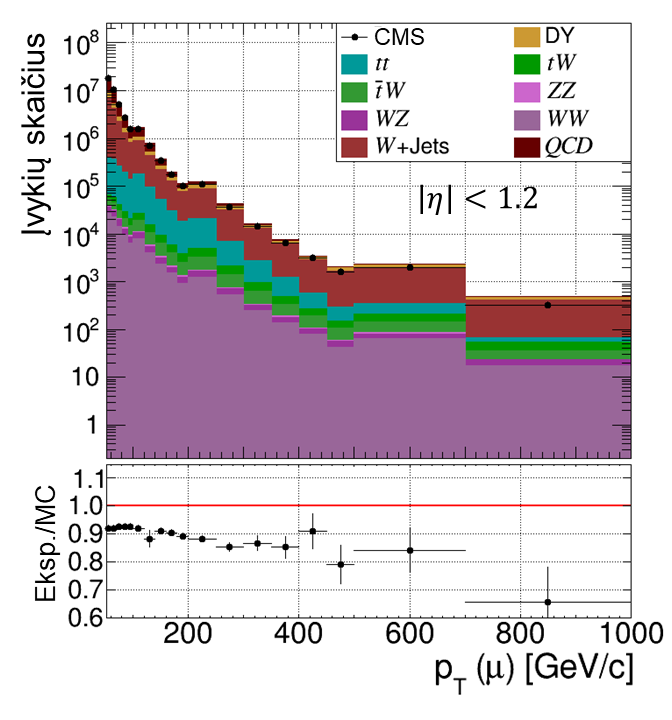
\includegraphics[width=0.49\textwidth]{Magistrinis/pT_mu_barrel.png}
	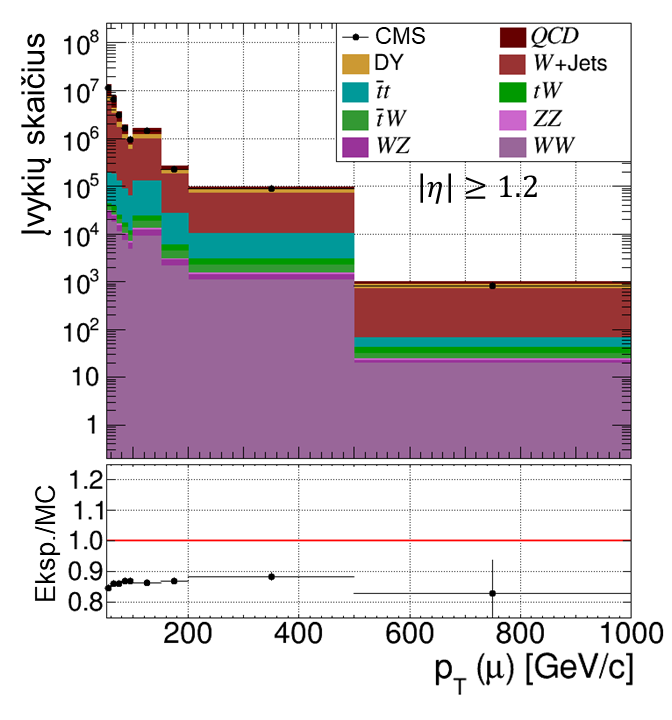
\includegraphics[width=0.49\textwidth]{Magistrinis/pT_mu_endcap.png}
	\caption{\label{fig:FRpT_mu}
		Klaidingo atpažinimo tikimybės įvertinimui skirtą atlaisvintą įvykių atranką praėjusių miuono objektų skersinio
		impulso pasiskirstymai CMS detektoriaus cilindrinėje (kairėje) ir antgalių (dešinėje) dalyse.
		Juodi brūkšniai vaizduoja tik statistinius neapibrėžtumus.}
	\vspace{1cm}
	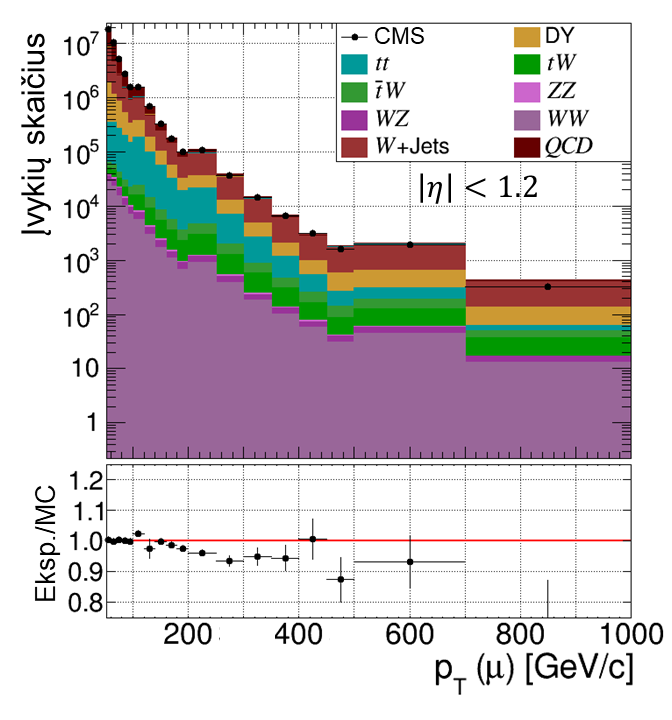
\includegraphics[width=0.49\textwidth]{Magistrinis/pT_mu_barrel_FIT.png}
	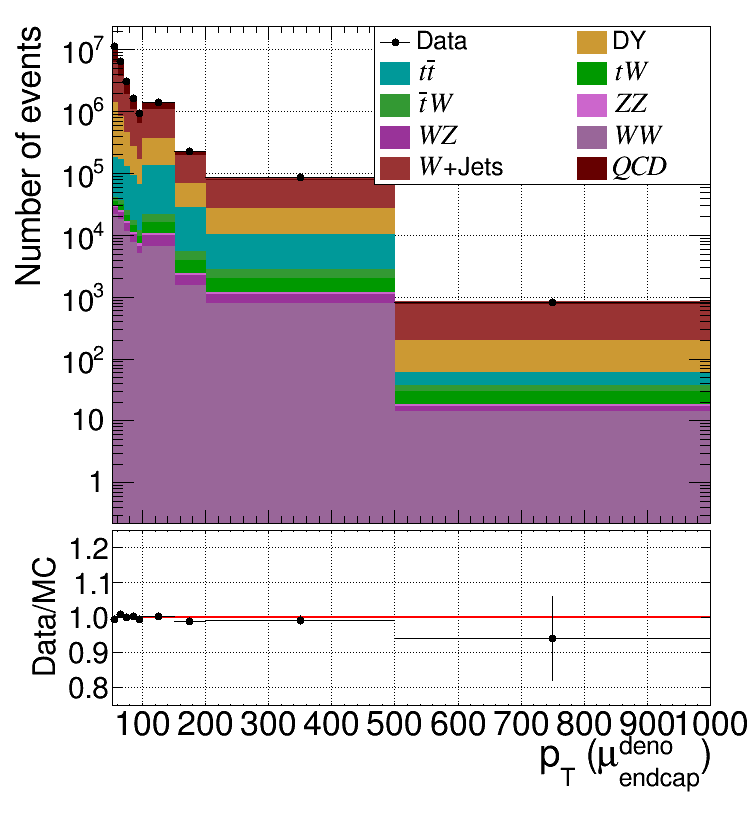
\includegraphics[width=0.49\textwidth]{Magistrinis/pT_mu_endcap_FIT.png}
	\caption{\label{fig:FRpT_muTFIT}
		Klaidingo atpažinimo tikimybės įvertinimui skirtą atlaisvintą įvykių atranką praėjusių miuono objektų skersinio
		impulso pasiskirstymai, pataisyti naudojant šablonų priderinimą.
		Kairėje pusėje pavaizduoti pasiskirstymai detektoriaus cilindrinei, o dešinėje -- antgalių dalims.
		Vaizduojami tik statistiniai neapibrėžtumai.}
\end{figure}

\begin{figure}[t!]
	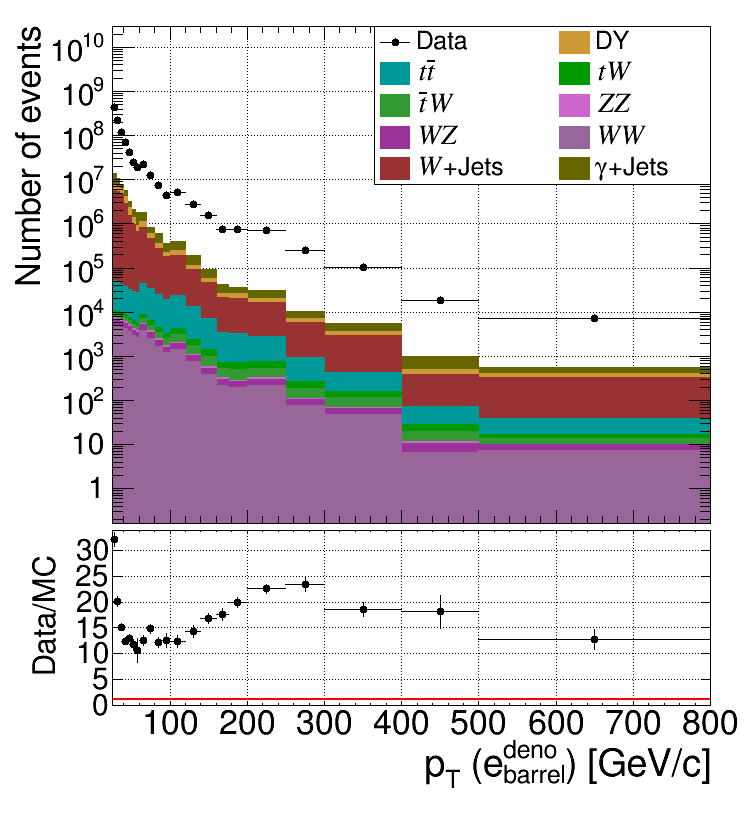
\includegraphics[width=0.49\textwidth]{Magistrinis/pT_e_barrel.png}
	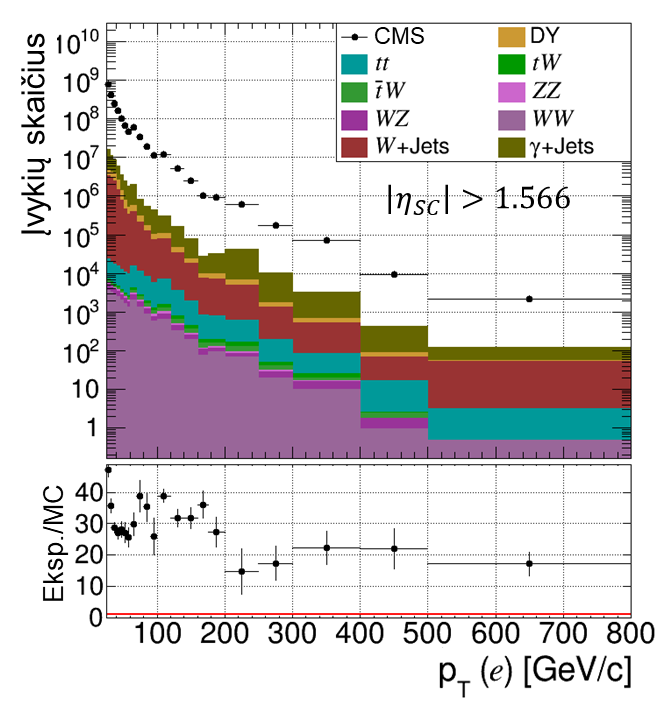
\includegraphics[width=0.49\textwidth]{Magistrinis/pT_e_endcap.png}
	\vspace{-0.5cm}
	\caption{\label{fig:FRpT_e}
		Klaidingo atpažinimo tikimybės įvertinimui skirtą atlaisvintą įvykių atranką praėjusių elektrono objektų skersinio
		impulso pasiskirstymai CMS detektoriaus cilindrinėje (kairėje) ir antgalių (dešinėje) dalyse.
		Vaizduojami tik statistiniai neapibrėžtumai.
		Visas grafikuose matomas skirtumas tarp išmatuoto ir modeliuoto pasiskirstymų buvo priskiriamas $\QCD$ procesui.}
\end{figure}

Tikslesnės klaidingo atpažinimo tikimybės, įvertintos kaip funkcijos nuo fizikinio objekto skersinio impulso ir pseudospartos,
yra pateiktos \ref{fig:FRmu} pav.\ miuono objektams ir \ref{fig:FRe} pav.\ elektrono objektams.
Buvo nustatyta, jog klaidingo atpažinimo tikimybė vidutiniškai yra didesnė, kai fizikinis objektas atkuriamas iš pataikymų į
CMS detektoriaus antgalius.
Taip pat tikimybė bendru atveju yra didesnė objektams su atkurtu didesniu skersiniu impulsu (išskyrus čiurkšlėms, imituojančioms
į cilindrą pataikiusius elektronus).
Miuono objektams klaidingo atpažinimo tikimybė kinta nuo $6\%$ iki $46\%$ cilindrinėje detektoriaus dalyje ir nuo $13\%$ iki
$72\%$ detektoriaus antgaliuose, o elektrono objektams -- nuo $2.5\%$ iki $6.5\%$ cilindrinėje ir nuo $3\%$ iki $24\%$ antgalių dalyje.

\begin{figure}[t!]
	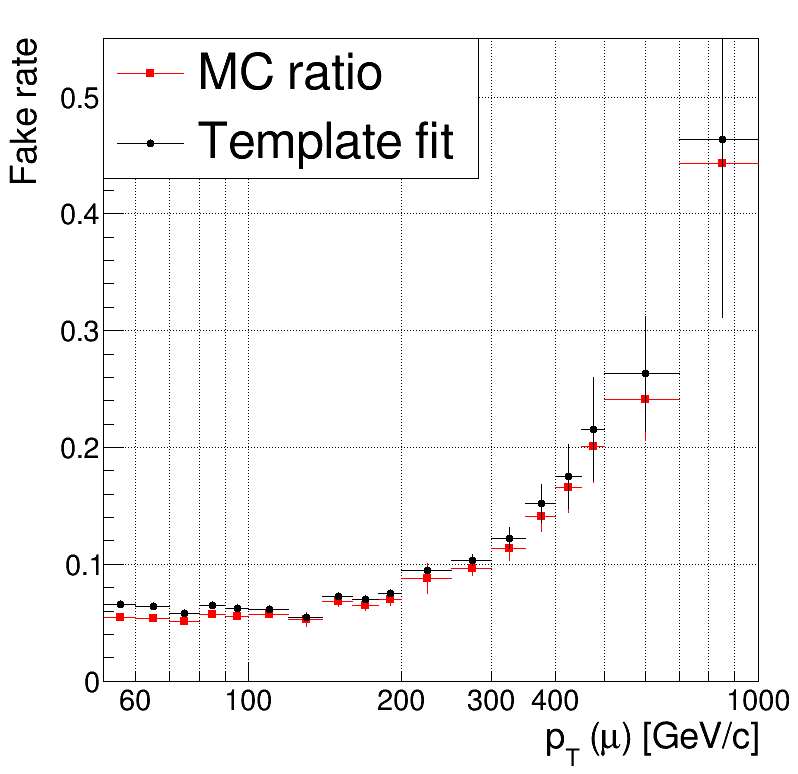
\includegraphics[width=0.49\textwidth]{Magistrinis/FRmu_barrel.png}
	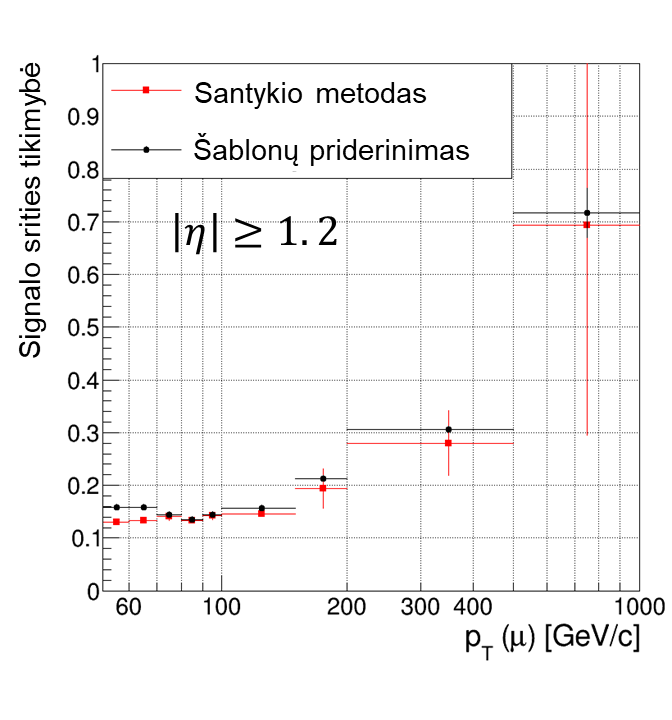
\includegraphics[width=0.49\textwidth]{Magistrinis/FRmu_endcap.png}
	\caption{\label{fig:FRmu}
		Miuono objektams įvertintos klaidingo atpažinimo tikimybės priklausomybė nuo objekto skersinio impulso.
		Kairėje pateiktas rezultatas trajektorijoms, einančioms per detektoriaus cilindrinę, o dešinėje -- per antgalių dalis.
		Skirtingos spalvos vaizduoja skirtingais metodais įvertintą tikimybę (žr.\ legendą).}
\end{figure}
\begin{figure}[t!]
	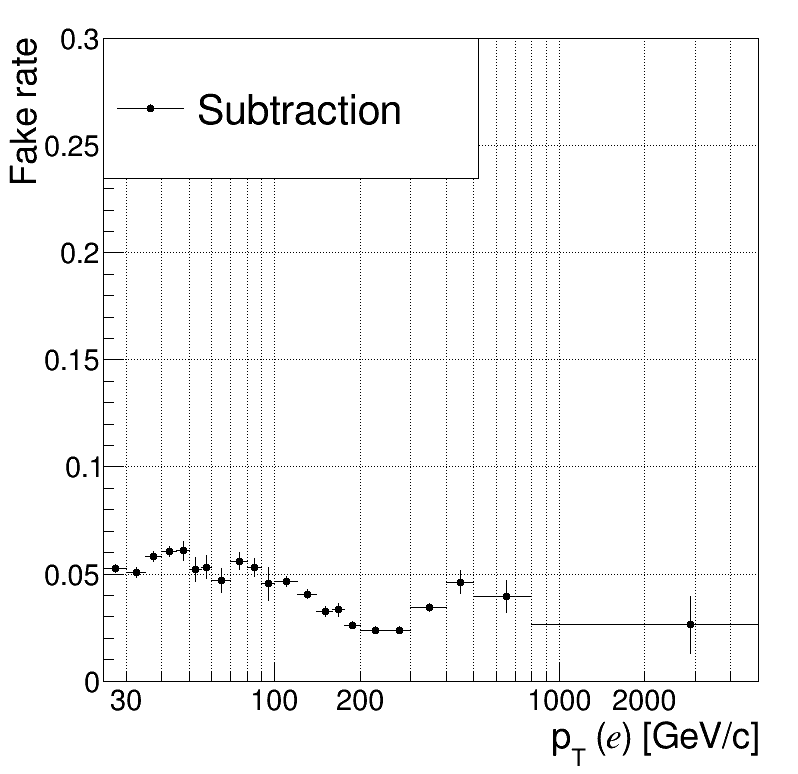
\includegraphics[width=0.49\textwidth]{Magistrinis/FRe_barrel.png}
	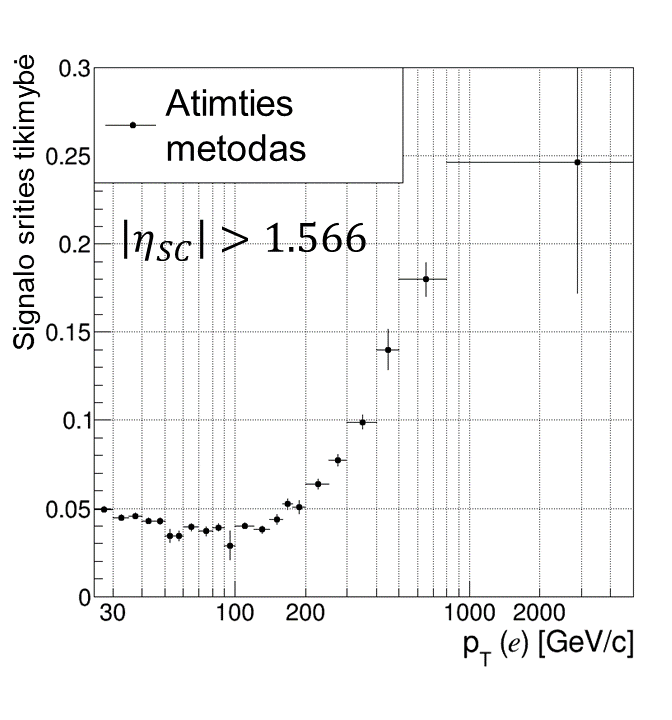
\includegraphics[width=0.49\textwidth]{Magistrinis/FRe_endcap.png}
	\caption{\label{fig:FRe}
		Elektrono objektams įvertintos klaidingo atpažinimo tikimybės priklausomybė nuo objekto skersinio impulso.
		Kairėje pateiktas rezultatas trajektorijoms, einančioms per detektoriaus cilindrinę, o dešinėje -- per antgalių dalis.}
\end{figure}

Apskaičiuotos klaidingo atpažinimo tikimybės buvo panaudotos įvertinant su $\QCD$ ir $\WJets$ procesais susijusių Drell-Yan
proceso triukšmo įvykių skaičių.
Klaidingo atpažinimo tikimybė kiekvienam griežtesniųjų atrankos kriterijų nepraėjusiam leptono objektui buvo pritaikoma atitinkamai pagal
jo skersinį impulsą ir pseudospartą.
\ref{fig:FRmu}~pav.\ pavaizduoti klaidingo atpažinimo tikimybės priklausomybės nuo skersinio impulso grafikai tampa
plokšti mažų skersinių impulsų srityse, todėl griežtesniųjų reikalavimų netenkinantiems miuono objektams su $\pT\!<\!52$~GeV buvo galima
naudoti tokią pačią klaidingo atpažinimo tikimybę, kaip ir objektams su $\pT\!=\!52$~GeV.
Triukšmo įvykių skaičiaus įverčiai buvo gauti iš \ref{table:jetSelection} lentelėje nurodytą atranką praėjusių įvykių
pasiskirstymų atimant su tikrais leptonais susijusius modeliuotus pasiskirstymus.

Gauti triukšmo įvykių skaičiaus pasiskirstymo įverčiai pateikti \ref{fig:JETmumu} ir \ref{fig:JETee} pav.\ atitinkamai
miuonų poros ir elektronų poros įvykiams.
Atkreiptinas dėmesys į paveikslų kairėse pusėse pavaizduotus $\WJets$ triukšmo pasiskirstymus, kurie turi ryškius
maksimumus ties $\sim\!90$~GeV.
Šie maksimumai yra susiję su $Z$ bozono skilimu į du leptonus ir neturi nieko bendro su $\WJets$ triukšmu.
Buvo padaryta išvada, kad $\WJets$ atranką praėjusių įvykių rinkinyje nepavyko teisingai atmesti įvykių, susijusių
su tikrais leptonais (ypatingai, Drell-Yan proceso).
Tai susiję su įvykių modeliavimo kokybe: kokybiškai sumodeliuoti prastai izoliuotus leptonus yra sudėtinga, todėl galima
tikėtis didesnių modeliavimo netikslumų įvykių rinkiniuose, kuriuose figūruoja signalo atrankos reikalavimų nepraeinantys leptonai.
Su $Z$ bozonu susiję maksimumai $\WJets$ triukšmo įverčiuose atsirado todėl, kad modeliuotas Drell-Yan proceso įvertis
nuvertina tikrąjį užregistruotų įvykių skaičių, t.y., įvertinant $\WJets$ įvykių skaičių atmetama per mažai Drell-Yan proceso
įvykių.
Panašų maksimumą, tik mažesnį, galima pastebėti ir \ref{fig:JETee} pav.\ pavaizduotame $\QCD$ proceso įvertyje.
Susidaro įspūdis, jog klaidingo atpažinimo metodas yra labai jautrus modeliavimo kokybei, nepaisant to, jog tai yra matavimu grįstas metodas.

\begin{figure}[!b]
	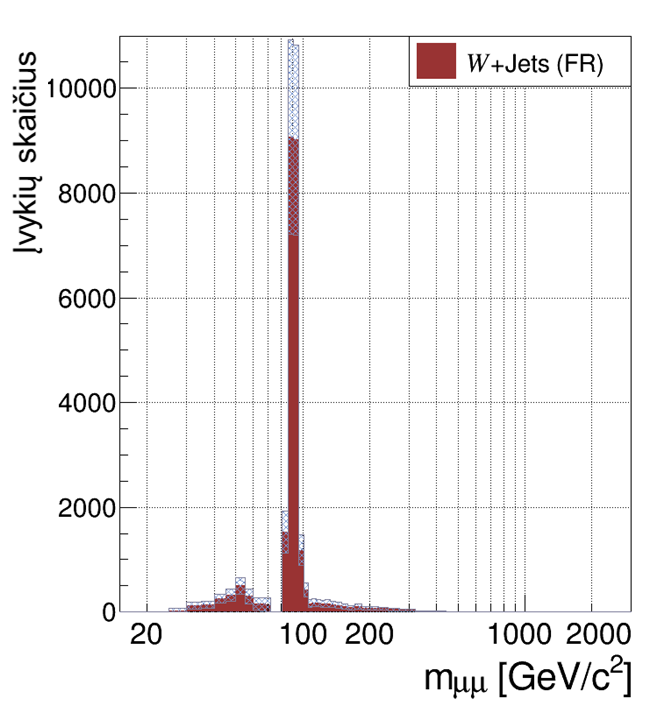
\includegraphics[width=0.48\textwidth]{Magistrinis/WJETest_mumu_os.png}
	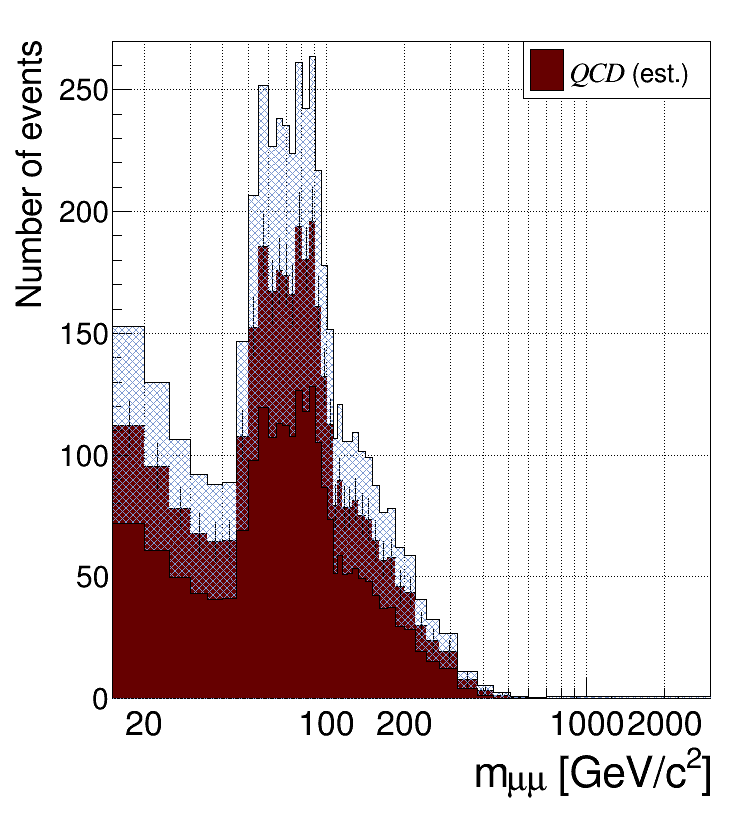
\includegraphics[width=0.48\textwidth]{Magistrinis/QCDest_mumu_final.png}
	\vspace{-0.3cm}
	\caption{\label{fig:JETmumu}
		Su klaidingai atpažintomis čiurkšlėmis susijusių $\WJets$ (kairėje) ir $\QCD$ (dešinėje) procesų indėliai į Drell-Yan proceso
		atranką praeinančių miuonų porų invariantinės masės pasiskirstymą.
		Mėlynos juostos žymi sumines paklaidas.
		Legendoje esantis užrašas \ltq{FR} žymi, kad įvertis gautas klaidingo atpažinimo metodu.
	}	
\end{figure}
\begin{figure}[!t]
	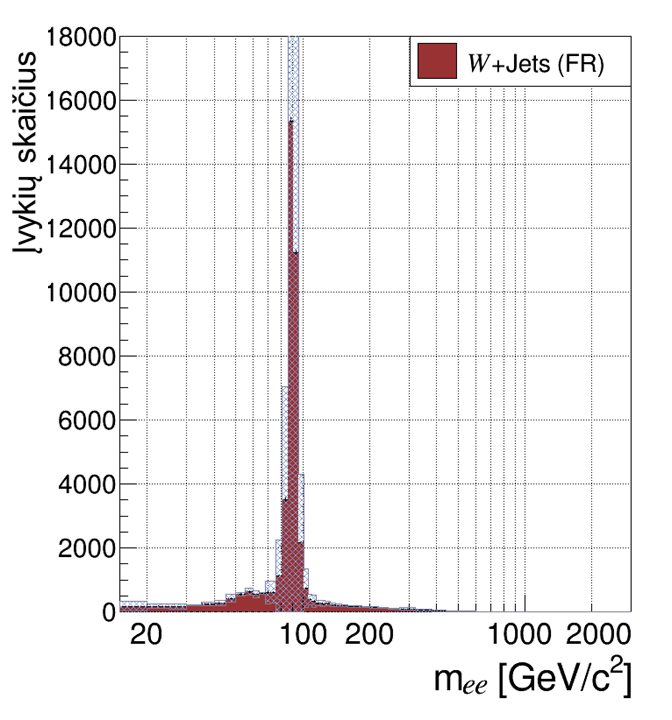
\includegraphics[width=0.48\textwidth]{Magistrinis/WJETest_ee_os.png}
	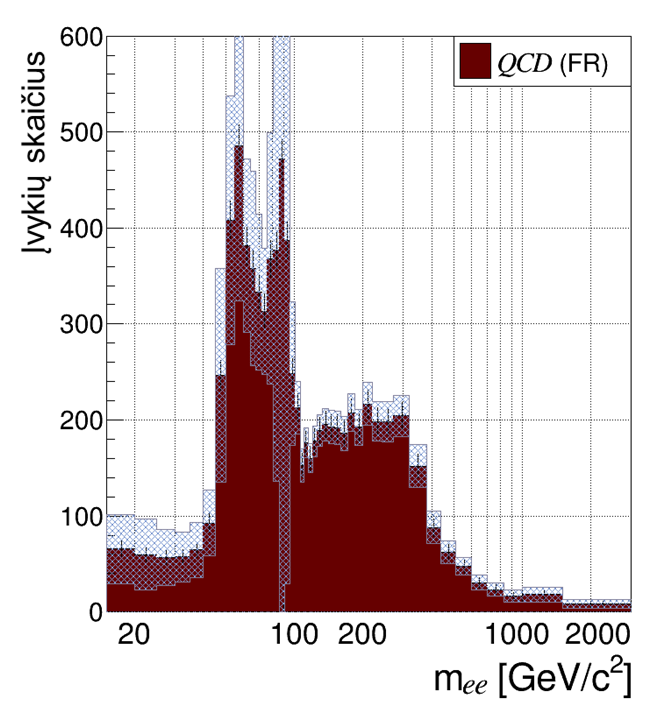
\includegraphics[width=0.48\textwidth]{Magistrinis/QCDest_ee_os.png}
	\vspace{-0.3cm}
	\captionof{figure}{\label{fig:JETee}
		Su klaidingai atpažintomis čiurkšlėmis susijusių $\WJets$ (kairėje) ir $\QCD$ (dešinėje) procesų indėliai į Drell-Yan proceso
		atranką praeinančių elektronų porų invariantinės masės pasiskirstymą.
		Mėlynos juostos žymi sumines paklaidas.
		Legendoje esantis užrašas \ltq{FR} žymi, kad įvertis gautas klaidingo atpažinimo metodu.
	}
\end{figure}

Dėl netikslaus modeliavimo gautus prastos kokybės įverčius buvo bandoma pataisyti naudojantis šablonų priderinimu.
Buvo daroma prielaida, kad su skirtingai procesais susijusių invariantinės masės pasiskirstymų forma sumodeliuojama
apytiksliai gerai, o prastai sumodeliuotas yra įvykių atrankos praėjimo efektyvumas, kuris nulemia bendrą atrinktų įvykių skaičių.
Tokiu atveju šablonų priderinimas gali padėti nustatyti realistiškesnį su skirtingais procesais susijusių įvykių skaičių,
kiekvienam procesui rasdamas pataisos daugiklį, kuris įskaito vidutinį efektyvumo nesutapimą.
Norint šį metodą pritaikyti, reikėjo gauti ir ieškomo proceso ($\QCD$ arba $\WJets$) šabloną, nes šablonų priderinimas
ieško geriausio skirtingų procesų šablonų sumos sutapimo su išmatuotu rezultatu.
Ieškomų procesų šablonai buvo gauti pakartojus analogišką klaidingo atpažinimo metodo procedūrą su įvykiais, kuriuose du
leptono objektai turi vienodą elektrinį krūvį.
Tokios atrankos turėtų nepraeiti Drell-Yan bei kitų procesų įvykiai, kuriuose sukuriami du priešingo krūvio leptonai, todėl šiuo
atveju netikslus modeliavimas įverčio turėtų taip smarkiai negadinti.
Pasinaudojant sumodeliuotais įvykių rinkiniais buvo įsitikinta, kad su $\WJets$ bei $\QCD$ procesais susijusių įvykių, kuriuose
atpažinti leptono objektai turi vienodus ir priešingus krūvius, pasiskirstymai paklaidų ribose skiriasi tik per konstantą.
Konstantą nustačius iš šablonų priderinimo, vienodo krūvio pasiskirstymus buvo galima naudoti kaip pagrindinei analizei skirtus
triukšmo įvykių skaičiaus įverčius, kuriuose leptono objektai yra priešingo krūvio (miuonų atveju) arba į jų krūvius nekreipiama
dėmesio (elektronų atveju).
Šablonų priderinimo rezultatai pavaizduoti \ref{fig:MassFit} pav.
Jį pritaikius skirtumas tarp eksperimento ir šablonų sumos masių srityje iki $300$~GeV neviršija $10\%$.

\begin{figure}[b!]
	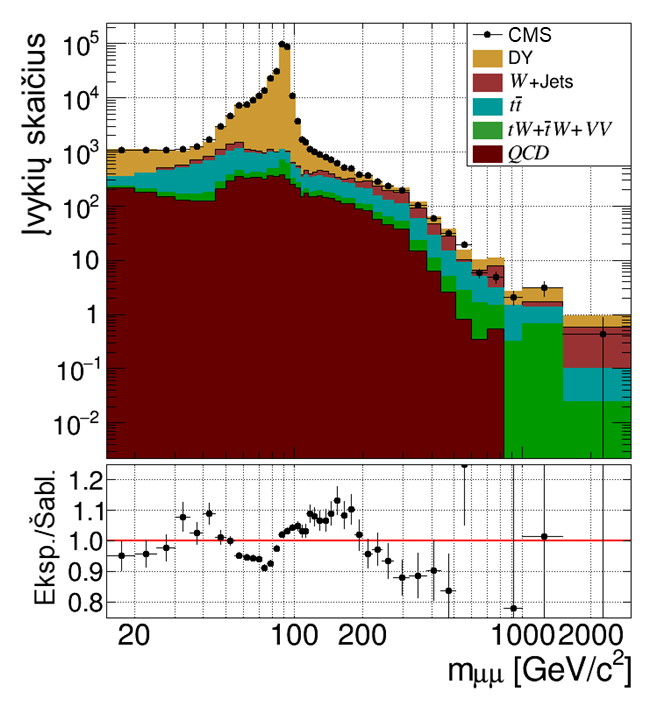
\includegraphics[width=0.325\textwidth]{Magistrinis/WJETmu_fit.png}
	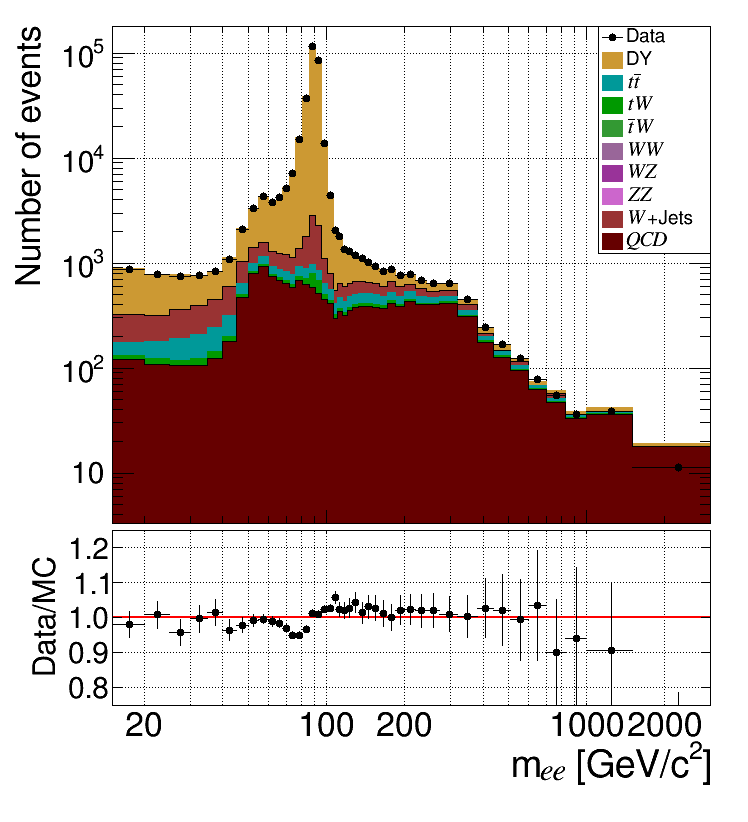
\includegraphics[width=0.325\textwidth]{Magistrinis/WJETe_fit.png}
	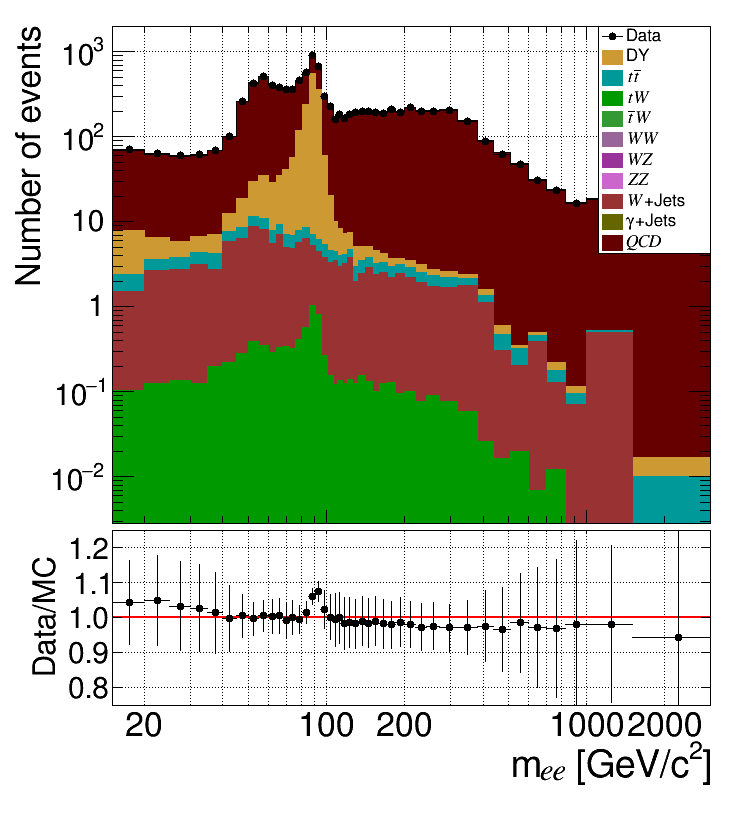
\includegraphics[width=0.325\textwidth]{Magistrinis/QCDe_fit.png}
	\vspace{-0.3cm}
	\caption{\label{fig:MassFit}
		Iš kairės į dešinę: $\WJets$ triukšmo įvykių skaičiui įvertinti miuonų ir elektronų kanaluose bei $\QCD$ įvykių
		skaičiui įvertinti elektronų kanale skirti išmatuoti pasiskirstymai bei prie jų priderinti šablonai.
		$\WJets$ (kairiajame ir viduriniame grafikuose) ir $\QCD$ (dešiniajame grafike) šablonai buvo gauti iš vienodo
		krūvio leptono objektų porų pasiskirstymų.}
\end{figure}

Iš šablonų priderinimo gauti triukšmo įvykių skaičiaus pasiskirstymo įverčiai pateikti \ref{fig:JETfit} pav.
Vienodo krūvio šablonai buvo naudojami trijų įverčių pagerinimui iš keturių: dviejų elektroną imituojančių čiurkšlių įverčiui
bei vienos elektroną arba miuoną imituojančios čiurkšlės įverčiams.
Siekiant atsižvelgti į naudotų šablonų galimai įneštus sisteminius nukrypimus, šiems įverčiams kaip papildoma sisteminio neapibrėžtumo
dedamoji, buvo įskaitomas skirtumas tarp pradinio triukšmo įvykių skaičiaus įverčio ir įverčio, gauto naudojant vienodo krūvio
šablonus.

Kaip galima pastebėti \ref{fig:JETfit} pav.\ viduryje pavaizduotame pasiskirstyme, Drell-Yan proceso modeliavimo
netikslumai paveikė net ir vienodo krūvio elektrono objektų porų pasiskirstymą -- lyginant su \ref{fig:JETee} pav.\ kairėje
pavaizduotu įverčiu, maksimumas ties $Z$ bozono mase sumažėjo, bet išliko labai ryškus.
Nors įvykių rinkinyje su vienodo krūvio leptono objektų poromis $Z$ maksimumo turėtų nebūti, dėl didelės tikimybės elektronui
priskirti neteisingą krūvį (ji siekia apie $1.5\%$ \cite{EleID}), į jį vis tiek patenka pakankamai daug Drell-Yan proceso įvykių,
kad šio proceso modeliavimo netobulumas paveiktų įverčio kokybę.
Sisteminė įvykių su viena elektroną imituojančia čiurkšle skaičiaus paklaida $75-105$~GeV masės srityje siekia $100\%$.
Ateityje šią problemą galimą būtų išspręsti pritaikius papildomą pataisą, įskaitančią tikimybę elektronui priskirti neteisingą krūvį,
tačiau dabar galima daryti išvadą, kad klaidingo atpažinimo metodas yra labiau tinkamas įvertinti triukšmams, kuriuose
čiurkšlė buvo klaidingai atpažinta kaip miuonas, nei kaip elektronas.

\begin{figure}[b!]
	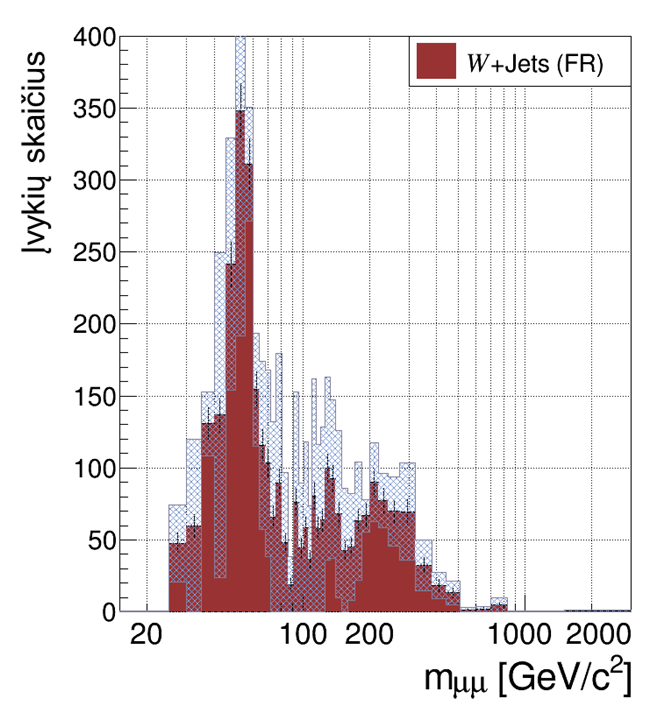
\includegraphics[width=0.325\textwidth]{Magistrinis/WJETest_mumu_final.png}
	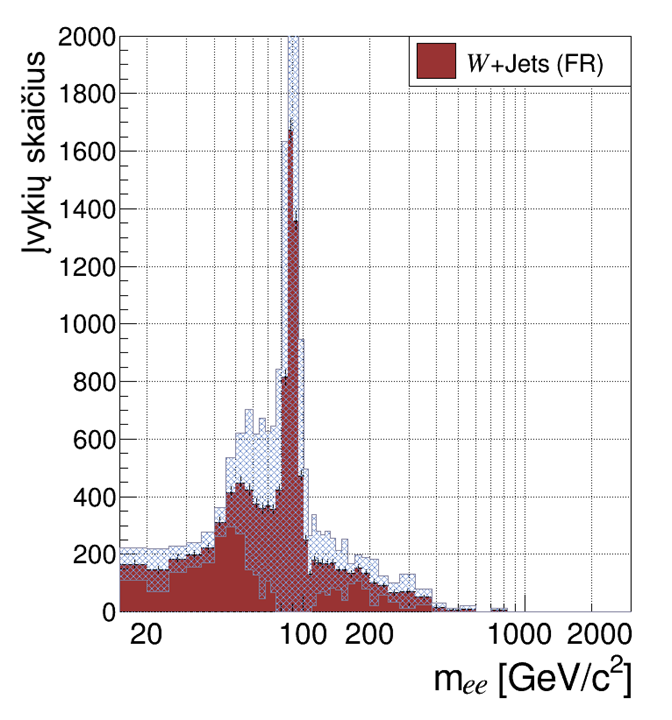
\includegraphics[width=0.325\textwidth]{Magistrinis/WJETest_ee_final.png}
	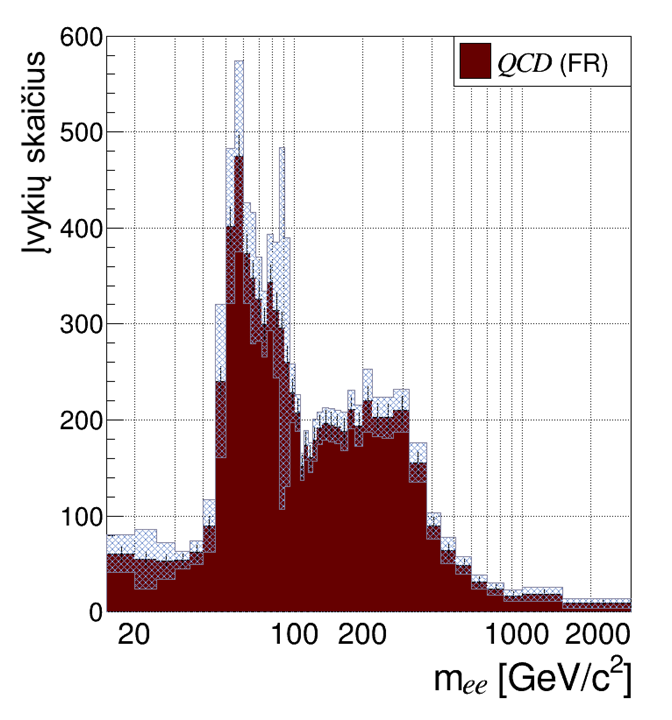
\includegraphics[width=0.325\textwidth]{Magistrinis/QCDest_ee_final.png}
	\vspace{-0.3cm}
	\caption{\label{fig:JETfit}
		Iš kairės į dešinę: $\WJets$ triukšmo įvykių skaičiaus miuonų ir elektronų kanaluose bei $\QCD$ įvykių
		skaičiaus elektronų kanale įverčiai, gauti taikant vienodo krūvio šablonus.
		Mėlynos juostos žymi sumines paklaidas.
		Legendoje esantys užrašai \ltq{FR} žymi, kad įverčiai gautas klaidingo atpažinimo metodu.
	}	
\end{figure}

Nustatyta, kad miuonų poros įvykių atranką praeina $6647\pm 82 \pm 2097$, o elektronų poros -- $18903\pm 137\pm 8333$
su klaidingai atpažintomis čiurkšlėmis susijusių įvykių.
Bendrai paėmus, net ir tų įverčių, kuriuose su $Z$ bozonu susijusio maksimumo neliko, sisteminės paklaidos yra ganėtinai didelės
ir siekia iki $54\%$.
Pagrindinė to priežastis -- didelis įverčio jautrumas klaidingo atpažinimo tikimybės pokyčiams (ypač įvykiams, kuriuose yra
dvi klaidingai atpažintos čiurkšlės, nes juose klaidingo atpažinimo tikimybė taikoma du kartus).
Vis dėlto, vien atitinkamų procesų modeliuotų įverčių statistinės paklaidos yra palyginamos arba net didesnės ir
siekia iki $90\%$ (o pabandžius apskaičiuoti sistemines paklaidas bendras neapibrėžtumas išaugtų dar labiau).
Tiesiogiai lyginti klaidingo atpažinimo metodu gautų triukšmo įvykių pasiskirstymų formą su modeliuotais atitinkamų procesų įverčiais
taip pat nėra didelės prasmės, nes modeliuoti šių procesų pasiskirstymai yra smarkiai netolydūs dėl prastos statistikos.
Taigi, galima sakyti, kad klaidingo atpažinimo metodo įverčiai yra tinkamesni naudojimui už modeliuotus.

Klaidingo atpažinimo metodą panaudojus $\emu$ metodo patikslinimui nustatyta, kad $6\%$ metodui naudotų įvykių yra susiję su
klaidingai atpažintomis čiurkšlėmis.
Su čiurkšlėmis susijusių triukšmo įvykių įverčiai, skirti $\emu$ metodui patikslinti, pateikiami 4 priede.

\ref{fig:MassFinal} pav.\ vaizduojami miuonų ir elektronų invariantinės masės pasiskirstymai palyginimai po klaidingo atpažinimo
metodo pritaikymo.
Grafikų apačioje esantys tamsiai ir šviesiai rudos spalvos pasiskirstymai vaizduoja atitinkamai dviejų ir vienos klaidingai
atpažintos čiurkšlės įvykius.
Palyginus su \ref{fig:MassBefore} pav.\ pateiktais grafikais galima pastebėti, kad ypatingai matavimu grįsti $\QCD$ įvykių
pasiskirstymai yra gerokai kokybiškesni už modeliuotus įverčius, kurie yra netolydūs dėl labai didelio proceso reakcijos
skerspjūvio ir labai mažos tikimybės praeiti signalo atranką (kokybiškesniam pasiskirstymui gauti
šių įvykių reikėtų sumodeliuoti bent 1000 kartų daugiau, bet tokiu atveju įvykių atranka truktų kelis mėnesius).
Klaidingo atpažinimo metodu įvertinti vienos klaidingai atpažintos čiurkšlės įvykių pasiskirstymai taip pat yra tolydesni,
tačiau elektronų įvertį dar reikėtų patobulinti panaikinant jau minėtą su klaidingai atpažintomis čiurkšlėmis nesusijusį maksimumą.
$\QCD$ ir $\WJets$ triukšmo įvykių skaičius sudaro $0.02\%$ visų miuonų poros įvykių ir $0.14\%$ visų elektronų poros įvykių,
todėl kalbėti apie bendrą išmatuoto ir suminio skirtingų procesų įverčių pasiskirstymų sutapimo pagerėjimą nėra didelės prasmės.
Gauti įverčiai (pritaikius reikalingą patobulinimą ateityje) bus panaudoti Drell-Yan signalo išskyrimui iš 2016 metais CERN CMS
detektoriaus užregistruotų duomenų.
Darbas bus tęsiamas bendradarbiaujant su tyrėjais iš JAV ir Pietų Korėjos.

\begin{figure}[b!]
	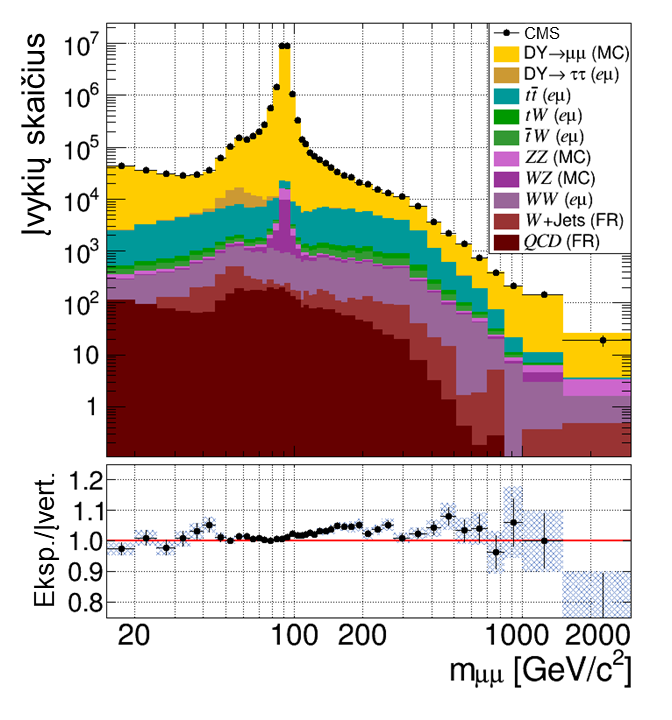
\includegraphics[width=0.49\textwidth]{Magistrinis/MuMumass_afterFR.png}
	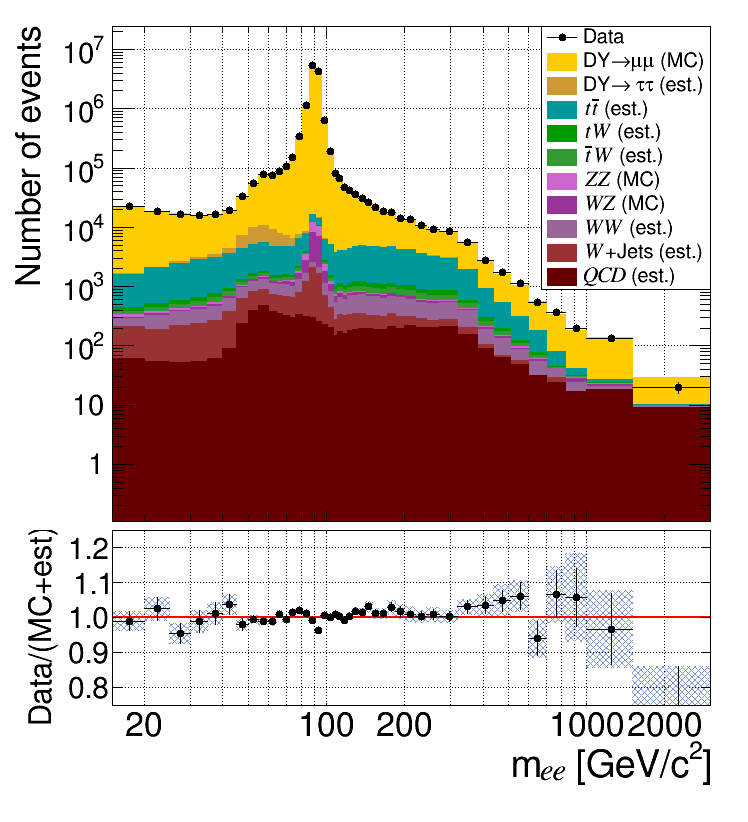
\includegraphics[width=0.49\textwidth]{Magistrinis/EEmass_afterFR.png}
	\vspace{-0.3cm}
	\caption{\label{fig:MassFinal}
		Miuonų (kairėje) ir elektronų (dešinėje) porų invariantinių masių pasiskirstymai pritaikius klaidingo atpažinimo metodą.
		Legendose esantys prierašai \ltq{FR} žymi klaidingo atpažinimo metodu gautus įverčius.
		Eksperimento ir įverčio santykio grafike esančios mėlynos juostos vaizduoja suminius (statistinius ir sisteminius)
		neapibrėžtumus.}
\end{figure}


\newpage
\section*{Išvados} \addcontentsline{toc}{section}{Išvados}
\begin{enumerate}
	\item Išsamios informacijos apie klaidingo atpažinimo metodą publikuotoje mokslinėje literatūroje yra mažai, o metodo
	įgyvendinimas turi nemažai variacijų, priklausančių nuo tyrimo pobūdžio.
	\item Klaidingo atpažinimo tikimybės nėra universalios ir priklauso nuo nuo tiriamų sričių apibrėžimų.
	\item Šablonų priderinimas duoda geresnį modeliuotų pasiskirstymų sutapimą su išmatuotaisiais eksperimento metu 
	nei normavimas pagal integruotą šviesį, todėl manoma, kad šio metodo taikymas klaidingai atpažintų čiurkšlių indėlio išskyrimui
	leidžia teisingiau įvertinti klaidingo atpažinimo tikimybę.
	\item Klaidingo atpažinimo metodu įvertinti triukšmo įvykių pasiskirstymai yra labai jautrūs procesų, susijusių su tikrais
	leptonais (ypač Drell-Yan proceso), modeliavimo kokybei.
	\item Drell-Yan proceso modeliavimo netikslumai labiausiai paveikė klaidingo atpažinimo metodu įvertintus įvykių pasiskirstymus,
	kuriuose tik viena čiurkšlė buvo klaidingai atpažinta kaip leptonas, taigi, klaidingo atpažinimo metodas yra tinkamesnis
	įvertinant triukšmo įvykių skaičių, kuriuose ne viena, o dvi čiurkšlės buvo klaidingai atpažintos kaip leptonai.
	\item Drell-Yan proceso modeliavimo netikslumų įtaką įvertintiems triukšmo įvykių pasiskirstymams galima sumažinti naudojant
	šablonų priderinimą.
	\item Šablonų priderinimo pritaikomumą įvykių su viena elektroną imituojančia čiurkšle skaičiaus įvertinimui riboja
	santykinai didelė tikimybė neteisingai nustatyti elektrono krūvį, taigi klaidingo atpažinimo metodas yra tinkamesnis
	įvertinti triukšmams, kuriuose čiurkšlė buvo klaidingai atpažinta kaip miuonas, nei kaip elektronas.
	\item Klaidingo atpažinimo metodu įvertinto triukšmo įvykių skaičiaus sisteminis neapibrėžtumas yra didelis dėl įverčio
	jautrumo klaidingo atpažinimo tikimybės įvertinimo tikslumui.
	\item Dėl didelio reakcijos skerspjūvio ir labai mažos tikimybės praeiti Drell-Yan signalo atranką, modeliuoti triukšmo
	įvykių, kuriuose čiurkšlės buvo klaidingai atpažintos kaip leptonai, pasiskirstymai yra netolydūs, o statistinė
	neapibrėžtis labai didelė, todėl laikoma, kad klaidingo atpažinimo metodu įvertinti triukšmo įvykių pasiskirstymai yra
	kokybiškesni. 
\end{enumerate}


\newpage
\addcontentsline{toc}{section}{Naudotos literatūros sąrašas}
\bibliography{KursinisDarbas}
\bibliographystyle{unsrt}


\newpage
\section*{Santrauka}
\addcontentsline{toc}{section}{Santrauka (LT)}
\begin{centering}
Marijus Ambrozas\\
\textbf{Drell-Yan proceso triukšmo įvykių skaičiaus įvertinimas klaidingo atpažinimo metodu}\\
\end{centering}
\vspace{0.5cm}

Didelės energijos protonų susidūrimų metu kvarkas iš vieno protono gali anihiliuoti su antikvarku iš kito ir pagaminti
leptono-antileptono porą.
Tokia reakcija yra vadinama Drell-Yan procesu.
Šiais laikais vykdomi didelio tikslumo Drell-Yan proceso diferencialinio reakcijos skerspjūvio matavimai leidžia
testuoti esamus teorinius modelius bei tikslinti protono sandaros aprašymą.
Eksperimentatoriai, tiriantys Drell-Yan procesą, ieško protonų susidūrimus fiksuojančiais detektoriais užregistruotų
priešingo krūvio leptonų porų.
Du priešingo krūvio leptonai gali susidaryti ir kitų pašalinių procesų metu, kuriuos Drell-Yan proceso tyrėjai vadina
triukšmo procesais.
Galimi ir tokie triukšmai, kai protonų susidūrimo metu susidariusios hadronų čiurkšlės detektoriuje imituoja leptonų pėdsakus.
Norint tiksliai išmatuoti Drell-Yan proceso reakcijos skerspjūvį, svarbu atsižvelgti į tokių procesų indėlį.

Šiame darbe pristatomas klaidingo atpažinimo metodas, kuris buvo naudojamas įvertinant su hadronų čiurkšlėmis susijusių
Drell-Yan proceso triukšmo įvykių skaičių.
Darbas buvo atliktas analizuojant 2016 metais CERN CMS eksperimento užregistruotus protonų susidūrimų duomenis,
atitinkančius $35.9$~\invfb integruotą šviesį ($\sim\!2 \cdot 10^{15}$ protonų susidūrimų).
Eksperimento metu užregistruotų duomenų interpretavimui buvo pasitelkiami CMS mokslinio kolektyvo paruošti
modeliuoti duomenų rinkiniai.
Vykdytą dviejų leptonų įvykių atranką praėjusiems elektronams ir miuonams buvo pritaikytos atitinkamai energijos ir
skersinio impulso matavimo skalių pataisos.
Modeliuotiems įvykiams buvo pritaikytas pataisų rinkinys, įskaitantis reikšmingiausius nesutapimus tarp realaus ir sumodeliuoto
eksperimento sąlygų.

Įvykdžius į Drell-Yan procesą panašių dviejų leptonų įvykių atranką buvo nustatinėjamas triukšmo įvykių skaičius, susijęs
su leptonais atpažintomis hadronų čiurkšlėmis.
Įvertintos tikimybės, kad klaidingai atpažintos čiurkšlės praeis Drell-Yan proceso leptonų (elektronų arba miuonų) atranką.
Naudojantis apskaičiuota tikimybe buvo įvertinta, kiek $\WJets$ (vienos čiurkšlės) ir $\QCD$ (keleto čiurkšlių)
įvykių galėjo praeiti Drell-Yan proceso atranką.
Nustatyta, jog su klaidingai atpažintomis hadronų čiurkšlėmis susiję įvykiai sudaro $0.02\%$ visų Drell-Yan proceso atranką
praėjusių miuonų poros įvykių ir $0.14\%$ elektronų poros įvykių.


\newpage
\section*{Summary}
\addcontentsline{toc}{section}{Santrauka (EN)}
\begin{centering}
Marijus Ambrozas\\
\textbf{Drell-Yan Process Background Estimation Using the Fake Rate Method}\\
\end{centering}
\vspace{0.5cm}

A lepton-antilepton pair production in proton-proton collisions is possible when a quark and an antiquark from colliding
protons annihilate.
This reaction is known as the Drell-Yan process.
Current precision measurements of Drell-Yan differential cross section have a high impact on the improvement
of proton structure description as well as provide various tests for the current theoretical models.
Scientific groups measure the Drell-Yan differential cross section by analyzing the proton-proton collision data and
searching for the opposite-charge lepton pairs.
There are several physics processes that may produce a similar footprint.
These additional processes are referred to as backgrounds.
Most background processes produce genuine opposite-charge lepton pairs, though, a few others include hadronic
jets, which were misreconstructed as leptons.
All the most significant backgound contributions must be taken into account in order to produce an accurate measurement.


This work presents an estimation of misreconstructed-jet-related Drell-Yan backgrounds using a data-driven fake rate method.
The work was performed by analyzing the proton-proton collision data collected by CERN CMS experiment in 2016.
The ammount of collected data corresponds to an integrated luminosity of $35.9$~\invfb ($\sim\!2 \cdot 10^{15}$ $pp$ collisions).
Simulated datasets provided by the CMS collaboration were used to interpret the collected detector data.
A dilepton event selection was performed after applying energy and momentum scale corrections to the reconstructed electron and muon
physical objects respectively.
A number of other corrections were applied to simulated event distributions in order to match the observed experimental conditions.

An estimation of the number of misreconstructed-jet-related background events was carried out having defined the event selection criteria.
A probability for a misreconstructed jet to pass the lepton identification requirements was estimated.
The misidintefication probability was then used to extract the number of $\WJets$ (single jet) and $\QCD$ (multiple jets)
events that pass the Drell-Yan dilepton selection.
It was evaluated, that misreconstructed jet events correspond to $0.02\%$ and $0.14\%$ of all the selected dimuon and dielectron
events respectively.


\newpage
\section*{Priedai} \addcontentsline{toc}{section}{Priedai}

\subsection*{1 priedas. Kai kurios antros (NLO) ir trečios (NNLO) eilės Drell-Yan proceso Feinmano diagramos}
Drell-Yan proceso Feinmano diagramos su antros eilės (NLO) kvantinės chromodinamikos pataisomis vaizduojamos \ref{fig:DYNLO} pav.
Diagramos su antros eilės (NLO) elektrosilpnosiomis pataisomis ir trečios eilės (NNLO) kvantinės chromodinamikos pataisomis
vaizduojamos \ref{fig:DYNNLO} pav.
Diagramose esančios nepažymėtos banguotos linijos vaizduoja virtualų fotoną arba $Z$ bozoną, susuktos linijos -- gliuonus, o
tiesios linijos su rodyklėmis -- elektrinį krūvį turinčius fermionus.
Diagramose laikas eina iš kairės į dešinę.

\begin{figure}[H]
	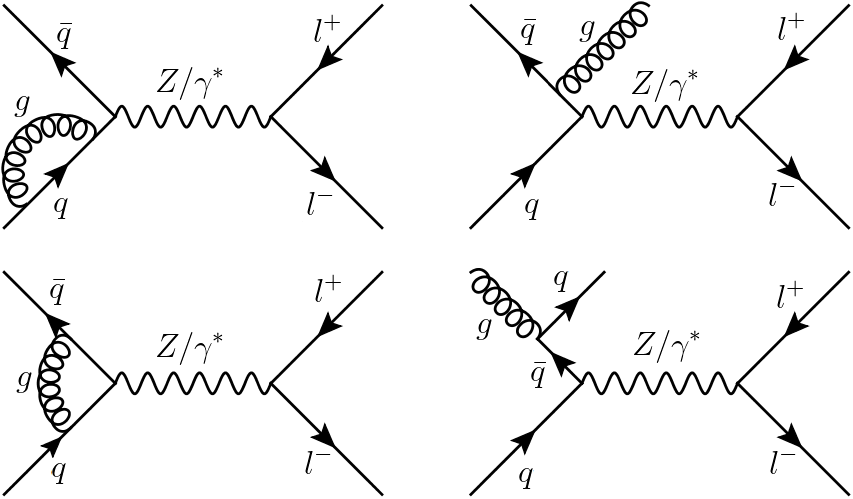
\includegraphics[width=0.5\textwidth]{Magistrinis/DY_NLO.png}
	\caption{\label{fig:DYNLO} Drell-Yan proceso Feinmano diagramos su kai kuriomis antros eilės (NLO) kvantinės chromodinamikos pataisomis.}
\end{figure}
\begin{figure}[H]
	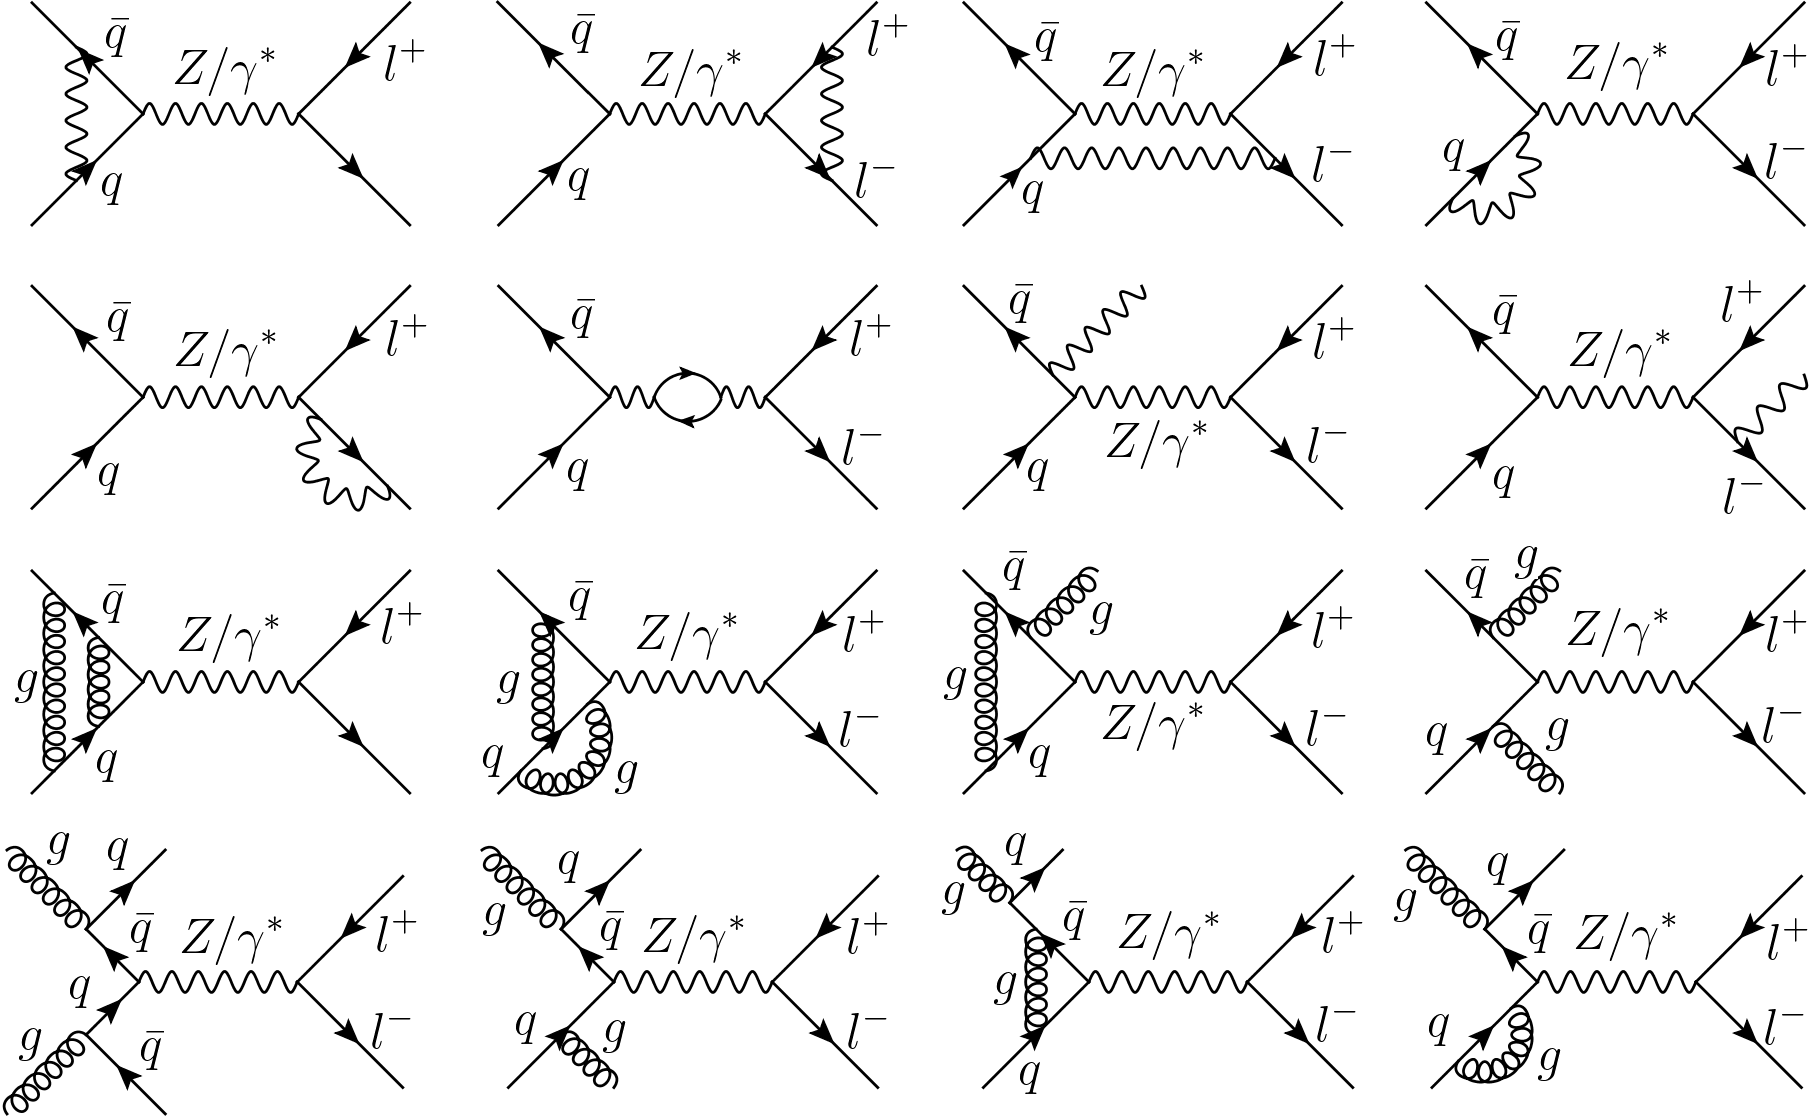
\includegraphics[width=0.9\textwidth]{Magistrinis/DY_NNLO.png}
	\caption{\label{fig:DYNNLO} Drell-Yan proceso Feinmano diagramos su kai kuriomis antros eilės (NLO) elektrosilpnosiomis ir trečios eilės
	(NNLO) kvantinės chromodinamikos pataisomis.}
\end{figure}


\subsection*{2 priedas. Elektrono \ltq{\ttt{MediumID}} kriterijai}
CMS elektrono ir fotono fizikinių objektų mokslinės grupės rekomenduojami vidutiniškai griežti elektrono objekto atpažinimo
kriterijai \ltq{\ttt{MediumID}} yra pateikti žemiau esančioje lentelėje.
Joje $\eta_{\mathrm{SC}}$ žymi CMS elektromagnetinio kalorimetro segmento, į kurį buvo pataikyta, pseudospartą,
$N_{\mathrm{MH}}$ žymi trūkstamų pataikymų CMS trekų detektoriuje skaičių.
Dvejetainis dydis \ttt{passConversionVeto} atspindi hipotezės, kad užregistruota trajektorija \textbf{neatitinka} elektrono,
atsiradusio fotono virsmo metu, patvirtinimą arba paneigimą.
Kiti atrankos kriterijuose naudojami dydžiai yra paaiškinti elektrono ir fotono fizikinių objektų mokslinės grupės paruoštame
straipsnyje \cite{EleID}.
\begin{table}[H]
	\begin{tabular}{|c|c|}
		\hline
		\multicolumn{2}{|c|}{\ltq{\ttt{MediumID}} kriterijai elektrono objektams} \\
		\hline
		\multirow{2}{15em}{\centering EM kalorimetro cilindre ($|\eta_{\mathrm{SC}}| \leqslant 1.479$)} &
			\multirow{2}{15em}{\centering EM kalorimetro antgaliuose ($|\eta_{\mathrm{SC}}| > 1.479$)} \\
		 & \\
		\hline
		$\sigma_{i\eta i\eta}<0.00998$ & $\sigma_{i\eta i\eta}<0.0298$ \\
		$|\Delta\eta_{\mathrm{in}}^{\mathrm{seed}}|<0.00311$ & $|\Delta\eta_{\mathrm{in}}^{\mathrm{seed}}|<0.00609$ \\
		$|\Delta\phi_{\mathrm{in}}|<0.103$ & $|\Delta\phi_{\mathrm{in}}|<0.045$ \\
		\multirow{2}{15em}{\centering$\displaystyle\frac{H}{E}<0.253$} &
			\multirow{2}{15em}{\centering$\displaystyle\frac{H}{E}<0.0878$} \\
		 & \\
		$I_{\mathrm{PF}}^{\mathrm{rel.}}<0.0695$ & $I_{\mathrm{PF}}^{\mathrm{rel.}}<0.0821$ \\
		\multirow{2}{15em}{\centering$\displaystyle \left| \frac{1}{E} - \frac{1}{p} \right|<0.134$} &
			\multirow{2}{15em}{\centering$\displaystyle \left| \frac{1}{E} - \frac{1}{p} \right|<0.13$} \\
		 & \\
		$N_{\mathrm{MH}}\leqslant1$ & $N_{\mathrm{MH}}\leqslant1$ \\
		\ttt{passConversionVeto} $=$ \ttt{True} & \ttt{passConversionVeto} $=$ \ttt{True} \\
		\hline
	\end{tabular}
\end{table}

\subsection*{3 priedas. Miuono objektų trajektorijos izoliuotumo parametro pasiskirstymų šablonų priderinimas}
Šablonų priderinimas buvo atliekamas atskirai į signalo ir kontrolinę sritis patekusiems miuono objektams.
Taip pat šablonai buvo išskaidyti pagal fizikinių objektų pseudospartą (į detektoriaus cilindrinę ir antgalių dalis)
bei skersinį impulsą (į tris ruožus: $\pT\!\in\!(52,70)$~GeV, $\pT\!\in\![70,100)$~GeV ir $\pT\!\in\![100,1000)$~GeV).
Iš viso šablonų priderinimas buvo atliktas su $12$ skirtingų pasiskirstymų.
Priderinti pasiskirstymai objektams signalo srityje yra pateikti \ref{fig:tFit_signal} pav., o kontrolinėje srityje --
\ref{fig:tFit_control} pav.

\begin{figure}[H]
	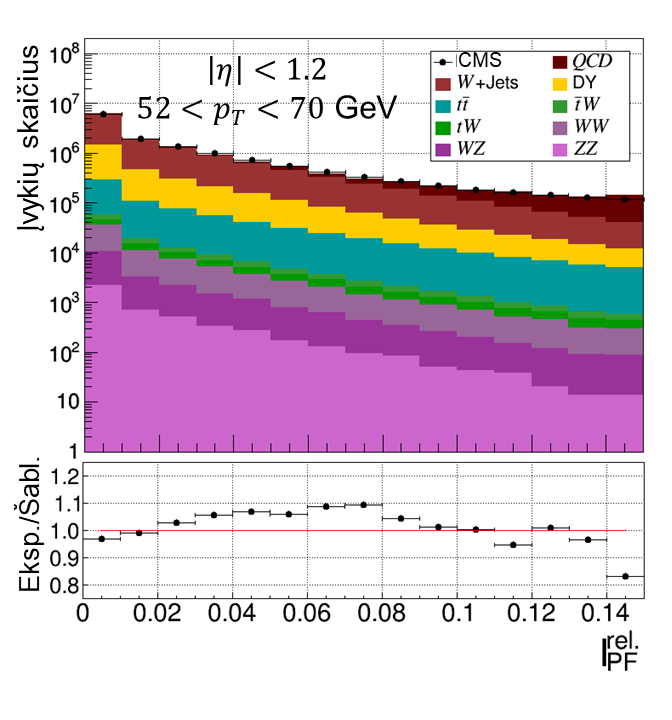
\includegraphics[width=0.42\textwidth]{Magistrinis/TFIT_nume_barrel_50to70.png}
	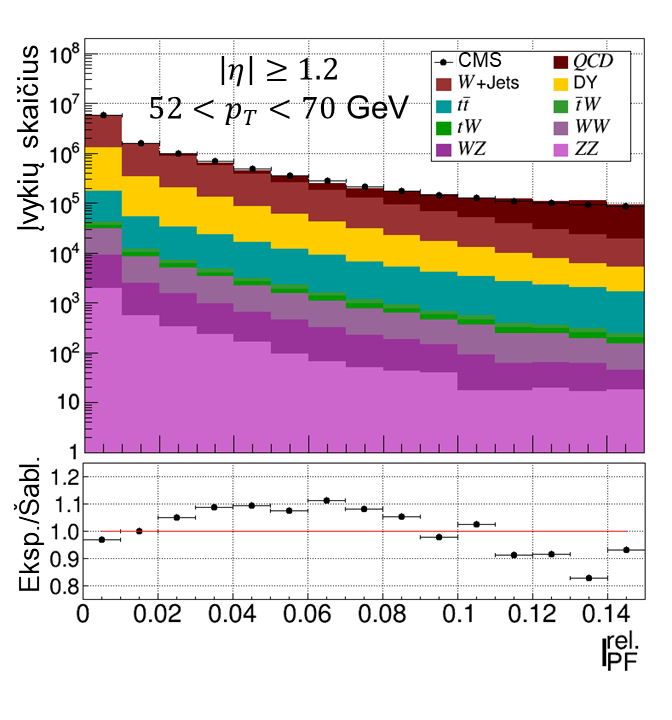
\includegraphics[width=0.42\textwidth]{Magistrinis/TFIT_nume_endcap_50to70.png}
\end{figure}
\vspace{-1cm}
\begin{figure}[H]
	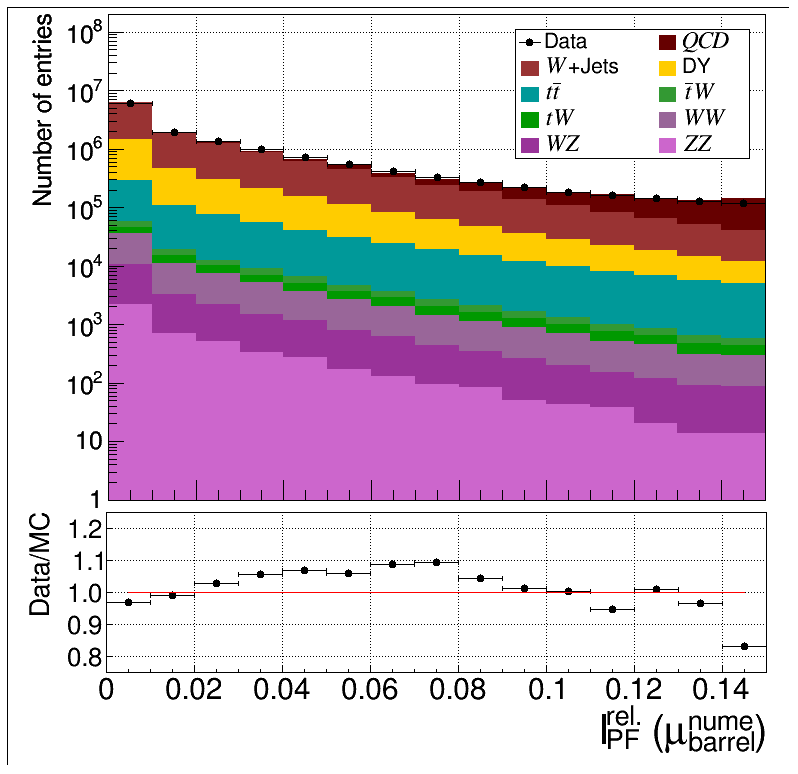
\includegraphics[width=0.42\textwidth]{Magistrinis/TFIT_nume_barrel_70to100.png}
	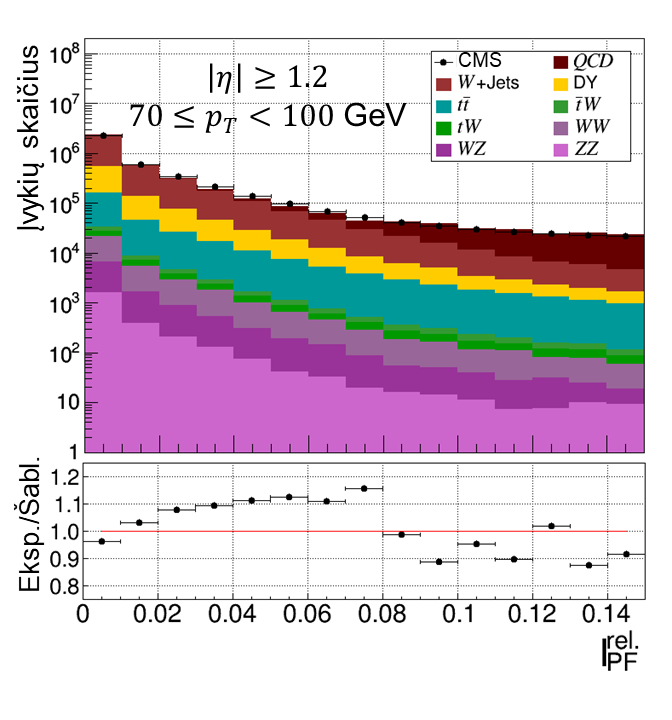
\includegraphics[width=0.42\textwidth]{Magistrinis/TFIT_nume_endcap_70to100.png}
\end{figure}
\vspace{-1cm}
\begin{figure}[H]
	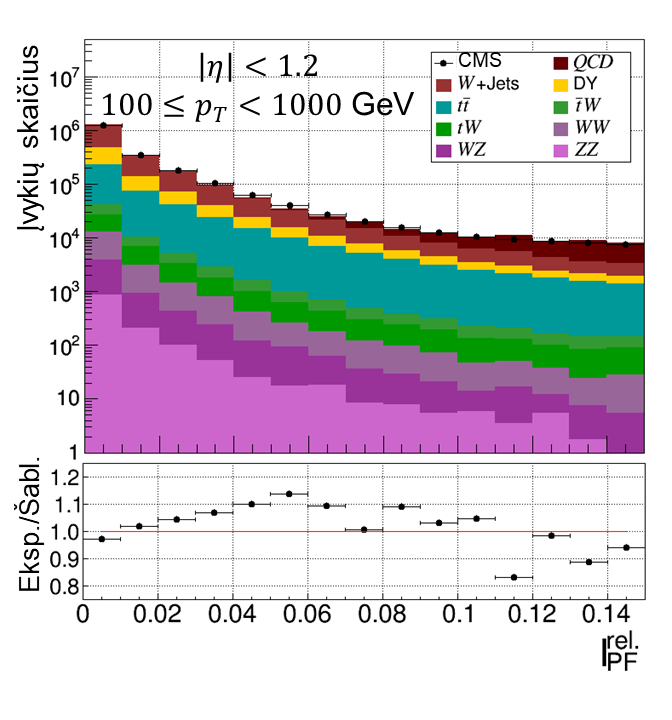
\includegraphics[width=0.42\textwidth]{Magistrinis/TFIT_nume_barrel_100to1000.png}
	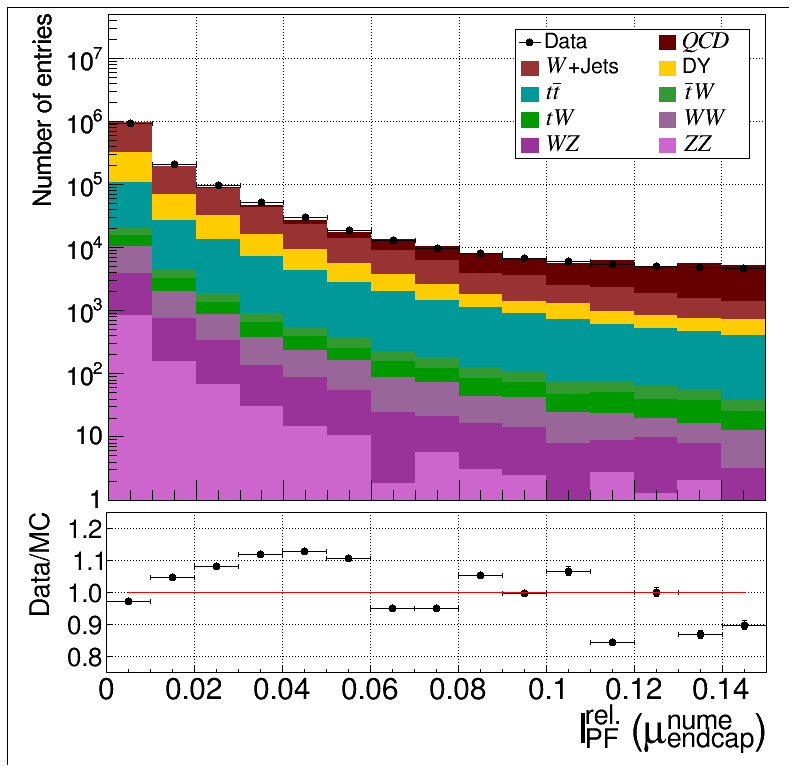
\includegraphics[width=0.42\textwidth]{Magistrinis/TFIT_nume_endcap_100to1000.png}
	\vspace{-0.7cm}
	\caption{\label{fig:tFit_signal}Prie matavimo priderinti į signalo sritį patekusių miuono objektų trajektorijos izoliuotumo
	parametrų pasiskirstymai skirtingose skersinio impulso ir pseudospartos srityse.
	Kairiame stulpelyje vaizduojami pasiskirstymai objektams detektoriaus cilindrinėje, o dešiniame -- antgalių dalyse.
	Eilutėse iš viršaus į apačią vaizduojami pasiskristymai atitinkamai miuono objektams su $\pT\!\in\!(52,70)$~GeV,
	$\pT\!\in\![70,100)$~GeV ir $\pT\!\in\![100,1000)$~GeV.}
\end{figure}

\begin{figure}[H]
	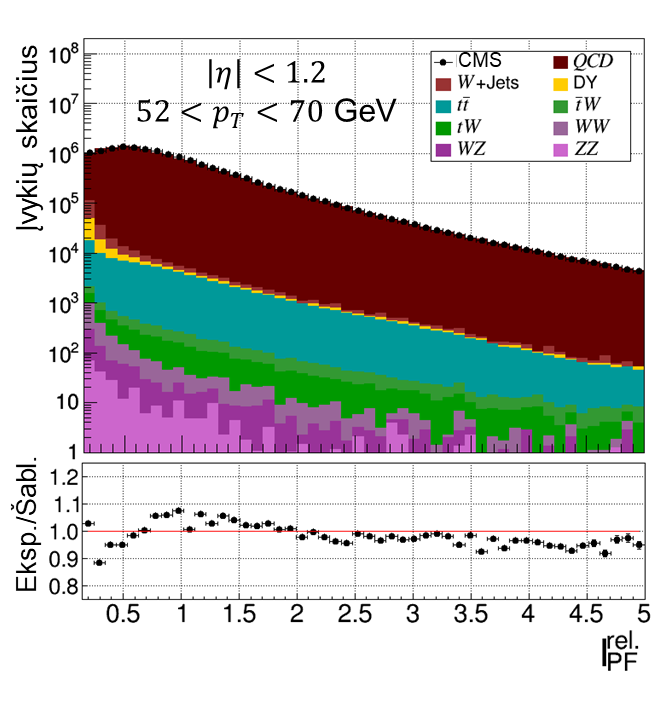
\includegraphics[width=0.42\textwidth]{Magistrinis/TFIT_ctrl_barrel_50to70.png}
	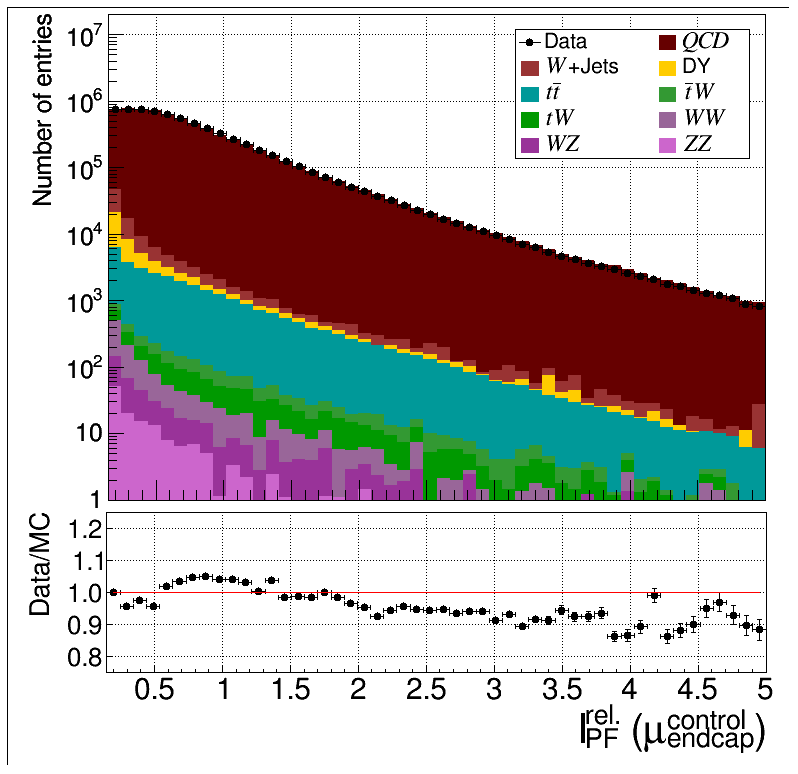
\includegraphics[width=0.42\textwidth]{Magistrinis/TFIT_ctrl_endcap_50to70.png}
\end{figure}
\vspace{-1cm}
\begin{figure}[H]
	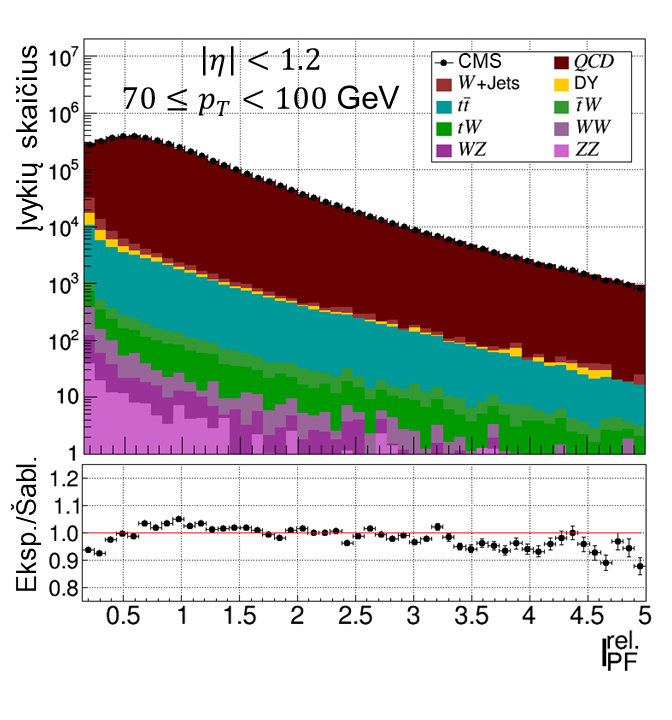
\includegraphics[width=0.42\textwidth]{Magistrinis/TFIT_ctrl_barrel_70to100.png}
	\includegraphics[width=0.42\textwidth]{Magistrinis/TFIT_ctrl_endcap_70to100.png}
\end{figure}
\vspace{-1cm}
\begin{figure}[H]
	\includegraphics[width=0.42\textwidth]{Magistrinis/TFIT_ctrl_barrel_100to1000.png}
	\includegraphics[width=0.42\textwidth]{Magistrinis/TFIT_ctrl_endcap_100to1000.png}
	\vspace{-0.7cm}
	\caption{\label{fig:tFit_control}Prie matavimo priderinti į kontrolinę sritį patekusių miuono objektų trajektorijos izoliuotumo
	parametrų pasiskirstymai skirtingose skersinio impulso ir pseudospartos srityse.
	Kairiame stulpelyje vaizduojami pasiskirstymai objektams detektoriaus cilindrinėje, o dešiniame -- antgalių dalyse.
	Eilutėse iš viršaus į apačią vaizduojami pasiskristymai atitinkamai miuono objektams su $\pT\!\in\!(52,70)$~GeV,
	$\pT\!\in\![70,100)$~GeV ir $\pT\!\in\![100,1000)$~GeV.}
\end{figure}


\section*{4 priedas. Su čiurkšlėmis susijusių triukšmo įvykių skaičiaus įvertinimas $\emu$ metodo patikslinimui}
Su viena ($\WJets$ ir dviem ($\QCD$) klaidingai atpažintomis čiurkšlėmis susijusių triukšmų indėliai į elektrono ir miuono
poros invariantinės masės pasiskirstymus, naudojamus taikant $\emu$ metodą, pateikti \ref{fig:emuBkg} pav.
\ref{fig:emuwFR} pav.\ pavaizduotas CMS detektoriumi išmatuoto elektrono ir miuono poros invariantinės masės pasiskirstymo
palyginimas su suminiu skirtingų procesų indėliu, susidedančiu iš modeliuotų įverčių procesams su tikrais leptonais ir 
klaidingo atpažinimo metodo įverčių procesams su klaidingai atpažintomis čiurkšlėmis.
Pritaikius klaidingo atpažinimo metodą, skirtumas tarp išmatuoto pasiskirstymo ir skirtingų procesų įverčių sumos invariantinės
masės srityje iki $700$~GeV nesiekia $8\%$.

\begin{figure}[H]
	\includegraphics[width=0.49\textwidth]{Magistrinis/WJETemu_est.png}
	\includegraphics[width=0.49\textwidth]{Magistrinis/QCDemu_est.png}
	\caption{\label{fig:emuBkg} Su klaidingai atpažintomis čiurkšlėmis susijusių $\WJets$ (kairėje) ir $\QCD$ dešinėje procesų
	indėliai į $\emu$ metodui naudojamą elektrono ir miuono poros invariantinės masės pasiskirstymą.
	Legendoje esantis užrašas \ltq{FR} žymi, kad įverčiai gauti klaidingo atpažinimo metodu.}
\end{figure}

\begin{figure}[H]
	\includegraphics[width=0.7\textwidth]{Magistrinis/emu_wFR.png}
	\caption{\label{fig:emuwFR} Elektrono ir miuono poros invariantinės masės pasiskirstymas, naudojamas $\emu$ metodui.
	Juodi taškai vaizduoja detektoriaus išmatuotą, o spalvoti stulpeliai -- modeliuotus (legendoje pažymėta \ltq{MC}) arba
	klaidingo atpažinimo metodu įvertintus (legendoje pažymėta \ltq{FR}) pasiskirstymus.}
\end{figure}


\newpage
\section*{Bibliografinis aprašas}
Marijus Ambrozas. Drell-Yan proceso triukšmo įvykių skaičiaus įvertinimas klaidingo atpažinimo metodu.
Teorinės fizikos ir astrofizikos magistro studijų programos baigiamasis darbas.
Vad.\ Andrius Juodagalvis. Vilnius: Vilniaus universitetas, Fizikos fakultetas, 2020.

\end{document}